\documentclass[12pt]{ociamthesis}  % default square logo 
%\documentclass[12pt,beltcrest]{ociamthesis} % use old belt crest logo
%\documentclass[12pt,shieldcrest]{ociamthesis} % use older shield crest logo

%load any additional packages
\usepackage{amssymb}
\usepackage{listings}

\usepackage{color}
 
\definecolor{codegreen}{rgb}{0,0.6,0}
\definecolor{codegray}{rgb}{0.5,0.5,0.5}
\definecolor{codepurple}{rgb}{0.58,0,0.82}
\definecolor{backcolour}{rgb}{0.95,0.95,0.92}

 
\lstdefinestyle{mystyle}{
    backgroundcolor=\color{backcolour},   
    commentstyle=\color{codegreen},
    keywordstyle=\color{magenta},
    numberstyle=\tiny\color{codegray},
    stringstyle=\color{codepurple},
    basicstyle=\footnotesize,
    breakatwhitespace=false,         
    breaklines=true,                 
    captionpos=b,                    
    keepspaces=true,                 
    numbers=left,                    
    numbersep=5pt,                  
    showspaces=false,                
    showstringspaces=false,
    showtabs=false,                  
    tabsize=2,
    language=sh
}

\lstset{style=mystyle}

%input macros (i.e. write your own macros file called mymacros.tex 
%and uncomment the next line)
%\include{mymacros}

\title{Modul Praktikum \\[1ex]     %your thesis title,
        Kecerdasan Buatan}   %note \\[1ex] is a line break in the title

\author{Rolly Maulana Awangga}             %your name
\college{0410118609\\[5ex]
Applied Bachelor of Informatics Engineering}  %your college

%\renewcommand{\submittedtext}{change the default text here if needed}
\degree{Politeknik Pos Indonesia}     %the degree
\degreedate{Bandung 2019}         %the degree date

%end the preamble and start the document
\begin{document}

%this baselineskip gives sufficient line spacing for an examiner to easily
%markup the thesis with comments
\baselineskip=18pt plus1pt

%set the number of sectioning levels that get number and appear in the contents
\setcounter{secnumdepth}{3}
\setcounter{tocdepth}{3}


\maketitle                  % create a title page from the preamble info
\include{section/dedication}        % include a dedication.tex file
\include{section/acknowlegements}   % include an acknowledgements.tex file
\include{section/abstract}          % include the abstract

\begin{romanpages}          % start roman page numbering
\tableofcontents            % generate and include a table of contents
\listoffigures              % generate and include a list of figures
\end{romanpages}            % end roman page numbering

%now include the files of latex for each of the chapters etc
\chapter{Mengenal Kecerdasan Buatan dan Scikit-Learn}
Buku umum yang digunakan adalah \cite{russell2016artificial} dan  
untuk sebelum UTS menggunakan buku \textit{Python Artificial Intelligence Projects for Beginners}\cite{eckroth2018python}.
Dengan praktek menggunakan python 3 dan editor anaconda dan library python scikit-learn.
Tujuan pembelajaran pada pertemuan pertama antara lain:
\begin{enumerate}
\item
Mengerti definisi kecerdasan buatan, sejarah kecerdasan buatan, perkembangan dan penggunaan di perusahaan
\item
Memahami cara instalasi dan pemakaian sci-kit learn
\item
Memahami cara penggunaan variabel explorer di spyder
\end{enumerate}
Tugas dengan cara dikumpulkan dengan pull request ke github dengan menggunakan latex pada repo yang dibuat oleh asisten riset.

\section{Teori}
Praktek teori penunjang yang dikerjakan :
\begin{enumerate}
\item
Buat Resume Definisi, Sejarah dan perkembangan Kecerdasan Buatan, dengan bahasa yang mudah dipahami dan dimengerti. Buatan sendiri bebas plagiat[hari ke 1](10)
\item
Buat Resume mengenai definisi supervised learning, klasifikasi, regresi dan unsupervised learning. Data set, training set dan testing set.[hari ke 1](10)
\end{enumerate}

\section{Instalasi}
Membuka https://scikit-learn.org/stable/tutorial/basic/tutorial.html. Dengan menggunakan bahasa yang mudah dimengerti dan bebas plagiat. 
Dan wajib skrinsut dari komputer sendiri.
\begin{enumerate}
\item
Instalasi library scikit dari anaconda, mencoba kompilasi dan uji coba ambil contoh kode dan lihat variabel explorer[hari ke 1](10)
\item
Mencoba Loading an example dataset, menjelaskan maksud dari tulisan tersebut dan mengartikan per baris[hari ke 1](10)
\item
Mencoba Learning and predicting, menjelaskan maksud dari tulisan tersebut dan mengartikan per baris[hari ke 2](10)
\item
mencoba Model persistence, menjelaskan maksud dari tulisan tersebut dan mengartikan per baris[hari ke 2](10)
\item 
Mencoba Conventions, menjelaskan maksud dari tulisan tersebut dan mengartikan per baris[hari ke 2](10)
\end{enumerate}


\section{Penanganan Error}
Dari percobaan yang dilakukan di atas, apabila mendapatkan error maka:

\begin{enumerate}
	\item
	skrinsut error[hari ke 2](10)
	\item
Tuliskan kode eror dan jenis errornya [hari ke 2](10)
	\item
Solusi pemecahan masalah error tersebut[hari ke 2](10)

\end{enumerate}


\section{Fathi Rabbani / 1164074}
\subsection{Teori}
\begin{enumerate}
\item
Sejarah dan Perkembangan Kecerdasan Buatan
\subitem
Sejarah dari sebuah Artificial Intelligence atau dalam Bahasa indonesianya diterjemahkan sebagai Kecerdasan Buatan adalah sebuah usaha untuk dapat memodelkan sebuah mesin agar dapat berfikir dan menirukan tingkah laku dan cara berfikir manusia, ada beberapa jenis dari kecerdasan buatan, yaitu :

\begin{itemize}
\item
Symbol Manipulating AI
\item
Nueral AI
\item
Neural Network
\end{itemize}
\subitem
Peneliti yang selalu disebutkan sebagai Bapak AI adalah Jhon McCharty  merupakan seorang dosen yang mengenalkan Kecerdasan Buatan kepada 2 lembaga penelitian hebat, yaitu Stanford Artificial Intelligence Laboratory dan MIT Artificial Intelligence Laboratory.
\subitem
Sedangkan perkembangan kecerdasan buatan saat ini sudah mencapai tahap dimana manusia mulai membuat sebuah robot yang dapat menirukan hampir 90 persen dari keseharian mereka, mulai dari bidang kesehatan, koki, pabrik, kantoran, hingga sebuah robot yang bertugas sebagai seorang pelayan di sebuah restoran. Dan dubai sebagai pengguna mobil tanpa pengemudi yang menerapkan AI dengan menggunakan data wilayah serta jarak kendaraan dengan pingir jalan.
\item
Definisi Supervised, Unsupervised Learning, Klasifikasi, Regresi serta Data, Training, Testing Set
\begin{itemize}
\item
Supervised learning merupakan sebuah pendekatan AI dengan latihan yang sudah dilakukan dengan sebuah data yang lengkap, dan memiliki variable yang dapat digunakan sebagai target sehingga dapat menujukan data agar menjadi kelompok dari sebuah data menjadi kelompok data yang baru.
\item
Unsupervised learning merupakan sebuah pendekatan AI tanpa menggunakan data yang lengkap dan ter-variable sehingga harus dilakukan pengelompokkan agar data tersebut dapat digunakan.
\item
Klasifikasi merupakan sebuah pengelompokkan suatu objek ke dalam kategori tertentu.
\item
Regresi merupakan pendekatan model matematika untuk mendeskripsikan hubungan dari beberapa variabel independen dengan variable dependen.
\item
Data Set, meupakan sebuah objek yang merepresentasikan data dan hubungannya di memory. 
\item
Training Set, subset untuk melatih model.
\item
Testing Set, subset untuk menguji model yang sudah dilatih.
\end{itemize}


\subsection{Praktikum}
\item
Instalasi Library Scikit dari Anaconda

\subitem
Pertama Download terlebih dahulu anaconda-nya di https://www.anaconda.com/distribution/ pilih Operating Sistem yang kalian gunakan. lalu setelah download Install dengan proses berikut :
\begin{itemize}
\item
Proses Instalasi Anaconda pada gambar \ref{proses2} hingga proses \ref{proses9}.
\item
Proses Instalasi Scikit-Learn dengan menggunakan Conda pada gambar \ref{proses10} hingga gambar \ref{proses12}.
\item
contoh dari Variable Explorer yang digunakan ada pada gambar \ref{proses14}.
\end{itemize}
\begin{figure}[ht]
\centerline{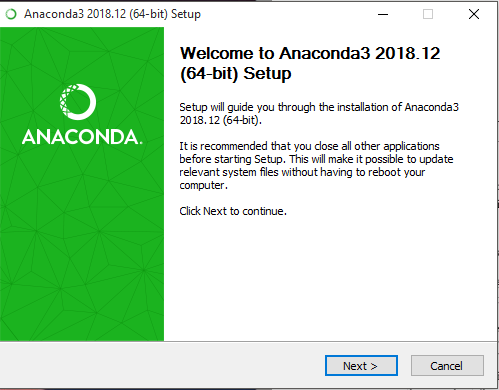
\includegraphics[width=1\textwidth]{figures/fathi/2.PNG}}
\caption{setelah membuka data instalasi klik next}
\label{proses2}

\centerline{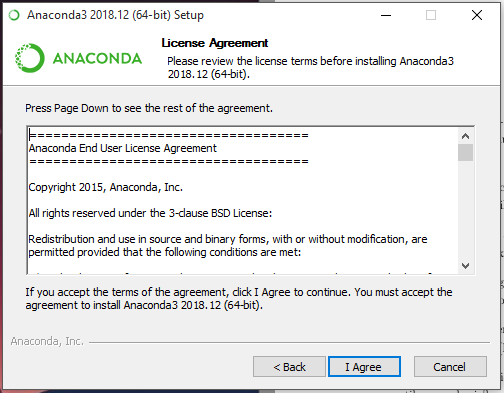
\includegraphics[width=1\textwidth]{figures/fathi/3.PNG}}
\caption{pilih i agree}
\label{proses3}
\end{figure}
\begin{figure}
\centerline{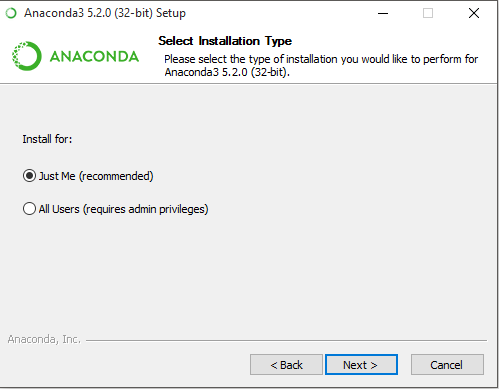
\includegraphics[width=1\textwidth]{figures/fathi/4.PNG}}
\caption{pilih instalasi Just Me}
\label{proses4}

\centerline{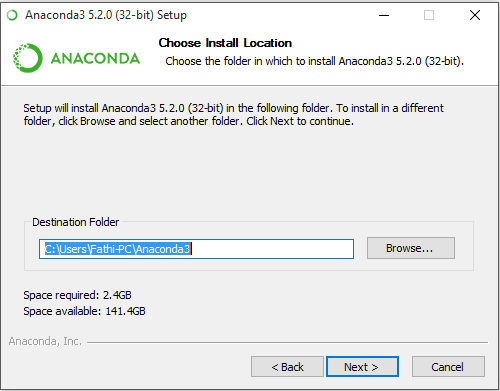
\includegraphics[width=1\textwidth]{figures/fathi/5.PNG}}
\caption{langsung saja next}
\label{proses5}
\end{figure}
\begin{figure}
\centerline{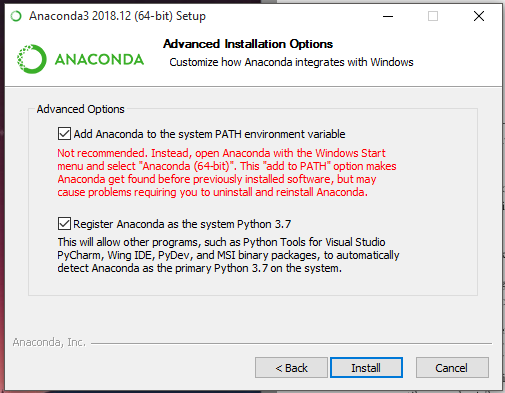
\includegraphics[width=1\textwidth]{figures/fathi/6.PNG}}
\caption{cek kedua pilihan tersebut}
\label{proses6}

\centerline{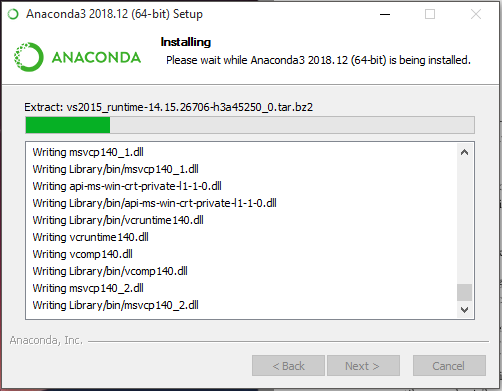
\includegraphics[width=1\textwidth]{figures/fathi/7.PNG}}
\caption{proses Instalasi}
\label{proses7}
\end{figure}
\begin{figure}
\centerline{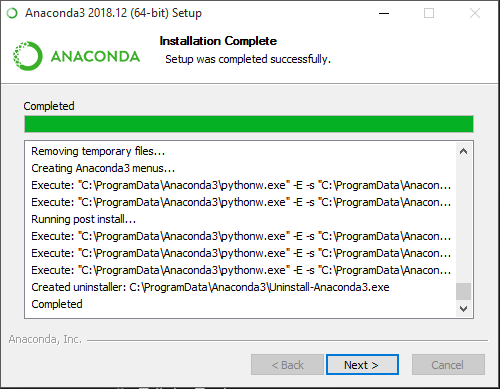
\includegraphics[width=1\textwidth]{figures/fathi/8.PNG}}
\caption{klik next}
\label{proses8}

\centerline{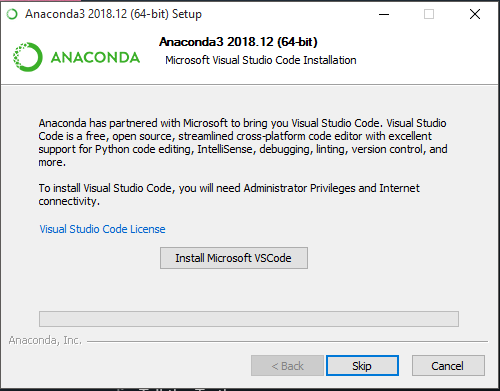
\includegraphics[width=1\textwidth]{figures/fathi/9.PNG}}
\caption{selesai instalasi anaconda}
\label{proses9}
\end{figure}
\begin{figure}
\centerline{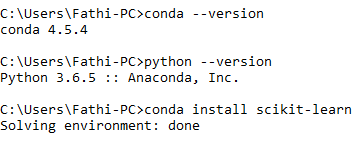
\includegraphics[width=1\textwidth]{figures/fathi/10.PNG}}
\caption{Instalasi SCIKIT dengan menggunakan anaconda}
\label{proses10}

\centerline{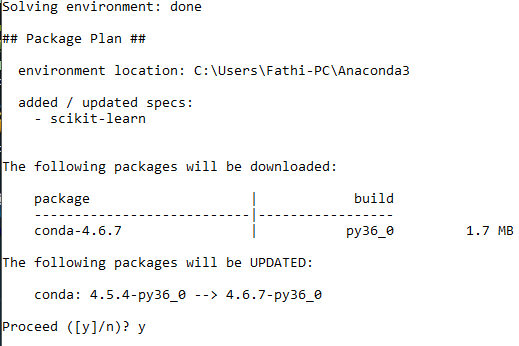
\includegraphics[width=1\textwidth]{figures/fathi/11.PNG}}
\caption{Konfirmasi Instalasi}
\label{proses11}
\end{figure}
\begin{figure}
\centerline{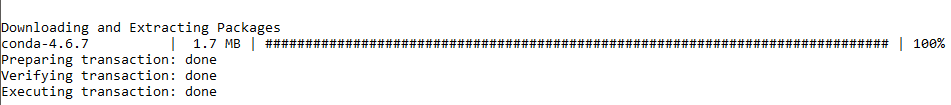
\includegraphics[width=1\textwidth]{figures/fathi/12.PNG}}
\caption{hasil dari instalasi SCIKIT}
\label{proses12}
\centerline{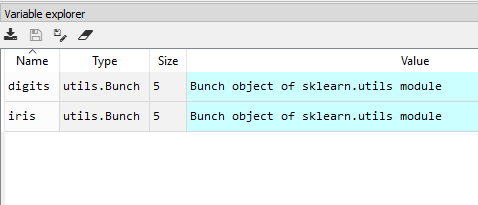
\includegraphics[width=1\textwidth]{figures/fathi/14.PNG}}
\caption{data variable explorer}
\label{proses14}
\end{figure}

\item
Load Example Dataset dan Menjeleaskan kegunakan barisan Code
\subitem
berikut ini adalah contoh dataset yang digunakan untuk melakukan compile ada pada gambar \ref{proses16} dan hasilnya ada pada gambar \ref{proses15}.

\begin{figure}
\centerline{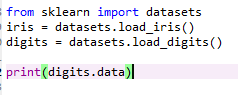
\includegraphics[width=1\textwidth]{figures/fathi/16.PNG}}
\caption{code example dataset yang digunakan}
\label{proses16}

\centerline{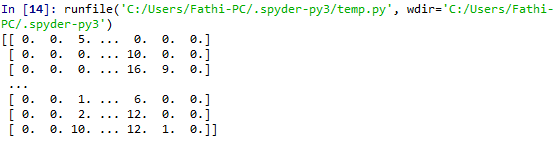
\includegraphics[width=1\textwidth]{figures/fathi/15.PNG}}
\caption{data hasil dari code example dataset yang digunakan}
\label{proses15}
\end{figure}
\begin{itemize}
\item
dari code yang dicoba diketahui bahwa data set yang digunakan adalah data yang diambil dari SKLEARN yang ada pada gambar \ref{proses16}.
\end{itemize}
\end{enumerate}

\chapter{Related Works}

Your related works, and your purpose and contribution which must be different as below.

\section{Cokro Edi Prawiro/ 1164069}

\subsection{Teori}
\begin{enumerate}
\item Jelaskan Apa Itu binari calssification drlengkapi ilustrasi gambar sendiri.\par
Binary Classification atau biominal adalah tugas mengklasifikasikan unsur usur dari himpunan yang diberikan kedalam kedua kelompok berdasarkan aturan klasifikasi yang telah ditetapkan. binari clasification juga dapat diartikan sebagai pembagi yang hanya memberikan dua pilihan contohnya benar dan salah atau klasifikasi tongkat panjang atau pendek. penjelasan lebih singkatnya binari classification merupakan kegiatam mengkelasifikasikan yang hanya memberikan dua class. contoh pada gambar \ref{c10} clasifikasi antara betuk kotak dan segitiga.

\item Jelaskan Apaitu supervised learning , unsupervised learning dan clusterring dengan ilustrasi gambar sendiri.\par
supervised learning adalah cara untuk mengklasifikasikan suatu objek atau data yang telah di tentukan kelas kelasnya contoh pada sayuran tumbuhan wortel termasuk yang mengandung vitamin A berarti tumbuhan wortel telah di kategorikan kedalam sayuran yang mengandung vitamin A. sedangkan kangkung mengandung zat besi yang berarti tumbuhan kangkung telah di kategorikan kedalam sayuran yang mengandung zat besi untuk lebih jelasnya dapat dilihat pada gambar \ref{c11}.\par
unsupervised learning merupakan cara untuk mengklasifikasi tanpa adanya kelas untuk menentukan jenisnya contoh sayuran berarti semua objek yang memiliki ciri ciri sayuran di kategorikan kedalam sayuran untuk lebih jelasnya dapat dilihat pada gambar \ref{c12}.\par
clustering merupakan peroses mengklasifikasikan yang berdasarkan suatu parameter dalam penentuannya contoh pada berat sayuran sayuran A memiliki berat 100 gr dan sayuran B memiliki berat 120 gr yang berarti berat sayuran dibagi dua parameter yaitu lebih kecil samadengan 100 gram dan lebih besar dari gram contoh pada gambar \ref{c13}.\par

\item Jelaskan apa itu evaluasi dan akurasi dan disertai ilustrasi contoh dengan gambar sendiri.\par
evaluasi adalah pengumpulan pengumpulan dan pengamatan dari berbagai macam bukti untuk mengukur dampak efektifitas dari suatu objek, program, atau proses berkaitan  dengan spesifikasi atau persyaratan yang telah di tetapkan sebelumnya. sedangkan akurasi itu sndiri merupakan bagian dari evaluasi yang merupakan ketepatan data terhadap suatu objek berdasarkan keriteria tertentu. kita dapat mengevaluasi seberapa baik model bekerja dengan mengukur akurasinya. ketepatan akan di definisikan sebagai presentase kasus yang di klasifikasikan dengan benar. hal ini berkaitan dengan confusion matrix pada materi selanjutnya. contoh evaluasi untuk membedakan burung dengan ayam terdapat parameter yaitu ukuran badan dan fungsi sayap pada hewan tersebut. lebih jelanya pada gambar \ref{c14} berikut:

\item Jelaskan bagaimana cara membuat Confusion Matrix, Buat confusion matrix sendiri.\par
Dalam pembuatan confusion matrix tentukan parameter atau objek yang akan di evaluasi contoh bunga melati , bunga mawar, dan bunga kenangan buat tabel dengan baris dan kolom berjumlah tiga kemudian tentukan nilai miring pada setiap kolom tersebut disini saya memberi nilai 30 dengan ketentuan setiap baris harus berisi nilai 30 nilai tersebut jika terbagi ke kolom lain maka jumlahnya harus bernilai 30 jika tidak berarti data tersebut tidak akurat. untuk lebih jelanya dapat dilihat pada gambar \ref{c15} berikut :

\item Jelaskan bagaimana K-fold cross validation bekerja dengan gambar ilustrasi contoh buatan sendiri.
K-fold Cross Validation merupakan cara untuk melatih suatu mesin dimana di dalammya terdapat data set yang dibagi menjadi dua yaitu untuk data testing dan data training contoh 1000 data merupakan data set dan 200 data digunakan untuk data testing kemudian 800 datanya digunakan untuk data training dimana data training tersebut digunakan untuk menentukan nilai bobot yang dimasukan kedalam rumus regresi linier. sedangkan nilai testing akan dijadikan nili inputan untuk rumus regresi linier. contohnya dapat dilihat pada gambar \ref{c16}  berikut :

\item Jelaskan Apa itu decision tree dengan gambar ilustrasi contoh buatan sendiri.\par
Decision tree (pohon keputusan) merupakan implementasi dari binari clasification dimana pada pohon keputusan akan terdapat root atau akar dan cabang cabangnya yang nilainya seperti if contoh pada root berisi nilai jenis kelamin, apakah perempuan pada cabang satu bernilai iya dan pada cabang dua bernilai tidak jika nilainya iya berarti jenis kelamminya perempuan dan jika tidak maka bernilai laki-laki.
agar lebih jelas dapat dilihat pada gambar \ref{c17}  decision tree berikut:

\item jelaskan apa itu information gain dan entropi dengan gambar ilustrasi buatan sendiri.\par
informasion gain merupakan informasi atau keriteria dalam pembagian sebuah objek contoh information gain pada laki-laki yaitu berrambut pendek, memiliki jakun, berjenggot, berkumis, dan mempunyai bahu yang lebar. pada kriteria tersebut seringkali terdapat bias misalkan ada perempuan yang berrambut pendek atau berkumis namun dari parameter tersebut dapat dilihat bahwa 60 persen parameter tersebut tepat pada sasaranya selama parameter itu bernilai tinggi untuk tepat maka dapat digunakan itulah information gain untuk lebih jelasnya dapat dilihat pada gambar \ref{c18}  berikut :\par
sedangkan entropi merupakan ukuran keacakan dari informasi semakin tinggi entropi maka semakin sulit dalam menentukan keputusan contoh dalam menentukan jenis kelamin semakin detail informasi maka akan semakin susah dalam menentukan keputusan.
\end{enumerate}

\subsection{Sikic-Learn /Cokro Edi Prawiro/1164069}
\begin{enumerate}
\item pada surcode pertama yang dapat dilihat pada gambar \ref{c19} pada baris pertama di tuliskan \begin{verbatim} import pandas as baso \end{verbatim} yang berarti mengimport library padas yang di inisialisasi namanya menjadi baso. selanjutnya pada baris ke dua codingan tersebut berisi \begin{verbatim} cireng = baso.read_csv
('E:\KULIAH\semester_6\AI\Buku\Chapter01\dataset\student-por.csv', sep=';')\end{verbatim} pada code tersebut terdapat variabel cireng yang berisi inisialisasi padas (baso) dengan aksi untuk membaca vfile csv yang terdapat pada direktori pada komputer kemudian terdapat sep samadengan titik koma yang berarti pemisah field di dalam vile tersebut merupakan titik koma. kemudian pada bagian akhir terdapat code len (nama variabel) yang berarti akan menghotung jumlah baris pada file tersebut. untuk hasilnya dapat dilihat pada gambar \ref{hasil1}

\begin{figure}[ht]
      \centerline{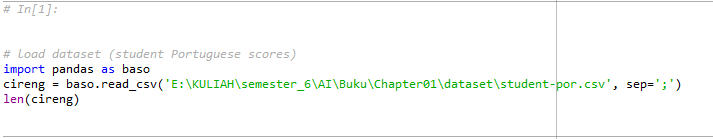
\includegraphics[width=1\textwidth]
      {figures/cokro/c19}}
      \caption{Source Code Load Dataset}
      \label{c19}
      \end{figure}

\begin{figure}[ht]
      \centerline{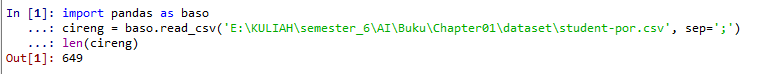
\includegraphics[width=1\textwidth]
      {figures/cokro/hasil1}}
      \caption{Hasil Load Dataset}
      \label{hasil1}
      \end{figure}

\item Pada code selanjutnya akan ditambahkan fungsi untuk lulus atau gagal yang dibuat berupa kolom kolom yang di dalammya terdapat nilai 0 dan 1 dimana 0 berarti gagal dan 1 berarti lulus. kemudian variabel pada codingan sebelumnya masih digunakan yaitu pada codingan berikut \begin{verbatim} cireng['pass'] = cireng.apply(lambda row:
 1 if (row['G1']+row['G2']+row['G3']) >= 35 else 0, axis=1) \end{verbatim}. dimana variabel cireng digunakan karena berisi nilai file csv kemudian dilakukan ekseskusi dengan parameter G1, G2, dan G3 dengan fungsi lambda yang berarti if bersarang atau if didalam if yang berarti nilai yang di eksekusi akan dilempar ke dalam setiap paramater sasuai dengan kriteria dan axis=1 yaitu nilai tersebut akan digunakan dari tiap baris data. sedangkan pada codingan \begin{verbatim} cireng = cireng.drop(['G1', 'G2', 'G3'], axis=1) \end{verbatim} variabel cireng di berikan aksi drop yaitu penurunan nilai pada bagian baris data. dan pada code cireng.head () yaitu untuk mengeksekusi codingan sebelumnya untuk lebih jelasnya dapat dilihat pada gambar \ref{c20} dan hasilnya seperti pada gambar \ref{hasil2} berikut :

\begin{figure}[ht]
      \centerline{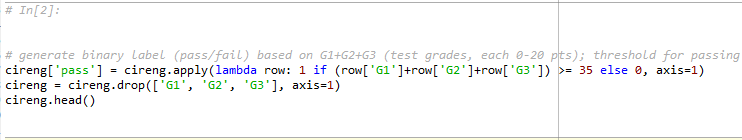
\includegraphics[width=1\textwidth]
      {figures/cokro/c20}}
      \caption{memberikan nilai satau atau nol}
      \label{c20}
      \end{figure}

\begin{figure}[ht]
      \centerline{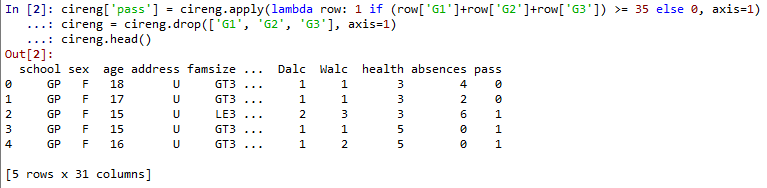
\includegraphics[width=1\textwidth]
      {figures/cokro/hasil2}}
      \caption{hasil dari memberikan nilai nol dan satu}
      \label{hasil2}
      \end{figure}

\item pada kodingan selanjutnya diguanakn untuk menambahkan nilai numerik berupa 0 dan 1 yang dirubah dari nilai tidak dan iya hal ini merupakan fungsi dari codingan get\_dummies pada baris pertama pada gambar \ref{c21} yang nilainya diambil dari variabel cireng yang telah di dekralasikan tadi banyaknya data numerik itu sendiri tergantung pada field dari kolom yang di camtumkan pada codingan dengan catatan field tersebut harus ada dalam data csv yang di import oleh codingan pertama tadi maka hasilnya akam merubah data dalam field tersebut menjadi 0 dan 1 untuk lebih jelasnya dapat di lihat pada gambar \ref{hasil3} berikut; 

\begin{figure}[ht]
      \centerline{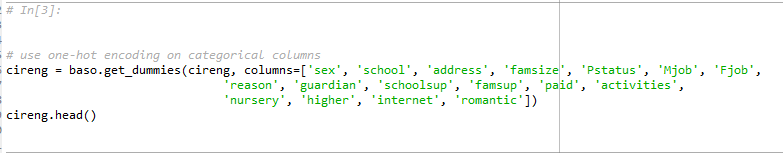
\includegraphics[width=1\textwidth]
      {figures/cokro/c21}}
      \caption{Penambahan nilai numerik}
      \label{c21}
      \end{figure}

\begin{figure}[ht]
      \centerline{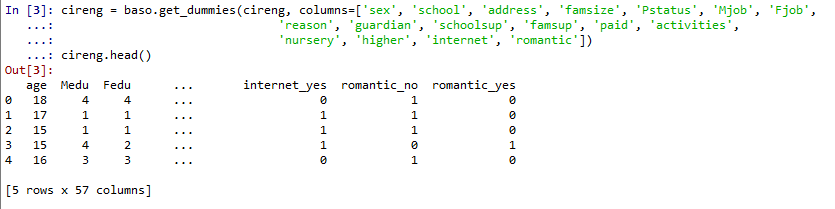
\includegraphics[width=1\textwidth]
      {figures/cokro/hasil3}}
      \caption{hasil Penambahan nilai numerik}
      \label{hasil3}
      \end{figure}

\item selanjutnya pada codingan selanjutnya yaitu menentukan data training dan data testing dari dataset dimana variabel cireng yang berisi data csv tadi dibuat perbandingan 500 untuk data training dan sisanya yaitu 149 digunakan untuk data testing hal ini di lakukan pada baris ke 1 sampai ke 3 pada gambar \ref{c22} kemudian nilai tersebut di turunkan  brdasarkan baris pada data set hal itu dapat dilihat pada baris ke 4 sampai ke 9 pada gambar \ref{c22} kemudian selanjutnya mengimport library numpy yang berguna untuk oprasi vektor dan matrix karna data diatas berupa data matrix maka library ini di gunakan. untuk hasilnya dapat dilihat pada gambar \ref{hasil4} dan \ref{hasilk4}

\begin{figure}[ht]
      \centerline{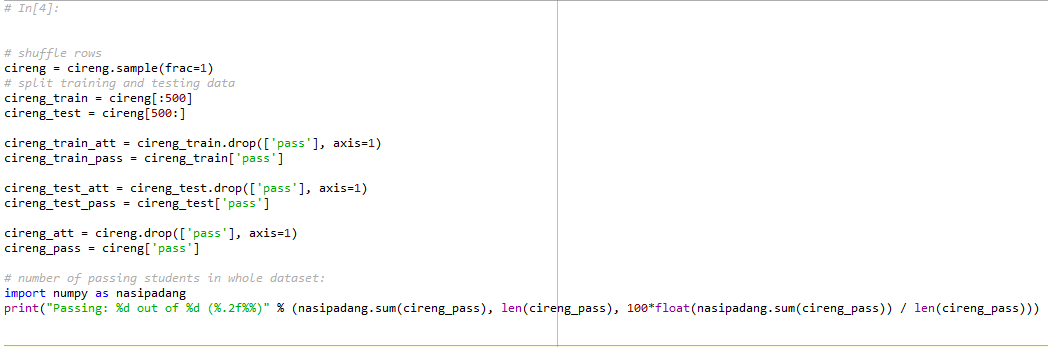
\includegraphics[width=1\textwidth]
      {figures/cokro/c22}}
      \caption{penentuan data training dan data testing}
      \label{c22}
      \end{figure}

\begin{figure}[ht]
      \centerline{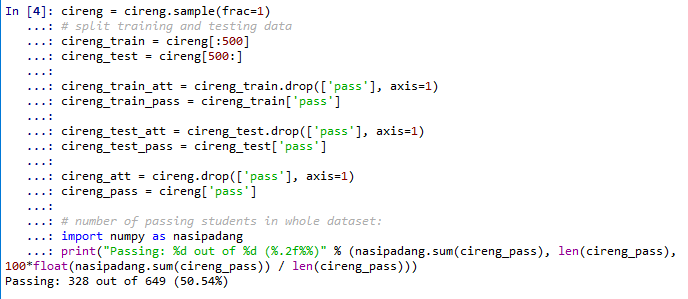
\includegraphics[width=1\textwidth]
      {figures/cokro/hasil4}}
      \caption{Hasil 1 penentuan data training dan data testing}
      \label{hasil4}
      \end{figure}

\begin{figure}[ht]
      \centerline{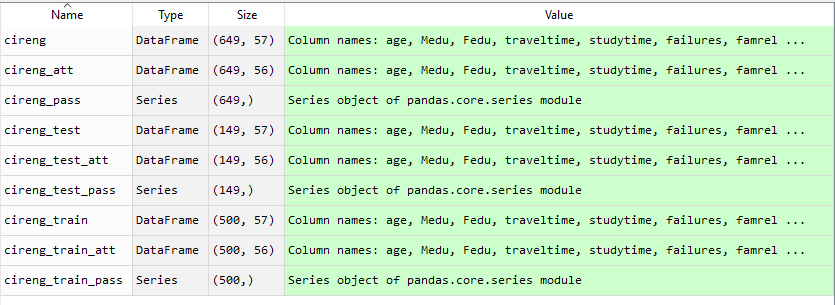
\includegraphics[width=1\textwidth]
      {figures/cokro/hasilk4}}
      \caption{hasil 2 penentuan data training dan data testing}
      \label{hasilk4}
      \end{figure}

\item selanjutnya yaitu membuat pohon keputusan dapat lebih jelasnya dapat di lihat pada gambar \ref{c23}. pada baris pertama yairu memasukan librari tree kemudian pada baris kedua dibuat variabel tempe dengan nilai DecisionTreeClasifier yang merupakan paket atau fungsi dari scikit-learn yang merupakan class yang mampu melakukan multi class. sedangkan max\_depth=5 merupakan untuk penyesuaian data terhadap pohon keputusan itu sndiri. untuk hasilnya dapat dilihat pada gambar \ref{hasil5}

\begin{figure}[ht]
      \centerline{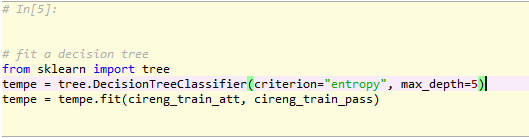
\includegraphics[width=1\textwidth]
      {figures/cokro/c23}}
      \caption{memberikan nilai pada pohon keputusan}
      \label{c23}
      \end{figure}

\begin{figure}[ht]
      \centerline{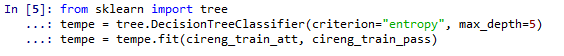
\includegraphics[width=1\textwidth]
      {figures/cokro/hasil5}}
      \caption{hasil memberikan nilai pada pohon keputusan}
      \label{hasil5}
      \end{figure}

\item selanjutnya yaitu pembuatan gambar dari pohon keputusan yang tadi di buta pada codingan sebelumnya pada baris pertama codingan ya itu mengimport library graphviz kemudian pada baris ke dua yaitu pemberian nilai pada variabel baru dot data nilainy diambil dari pembuatan puhon keputusan tadi kemudian di tentukannya nilai benar dan salah dari codingan tersebut setelah itu dibuatlah sebuah variabel untuk menampung hasil eksekusi tersebut kemudian variabel tersebut di running untuk lebih jelasnya dapat di lihat pada gambar \ref{c24} kemudian hasilnya dapat dilihat pada gambar \ref{hasil6}.

\begin{figure}[ht]
      \centerline{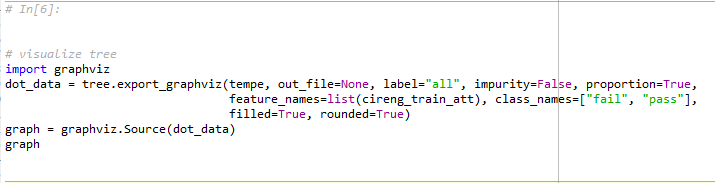
\includegraphics[width=1\textwidth]
      {figures/cokro/c24}}
      \caption{pembuatan diagram puhon keputusan}
      \label{c24}
      \end{figure}

\begin{figure}[ht]
      \centerline{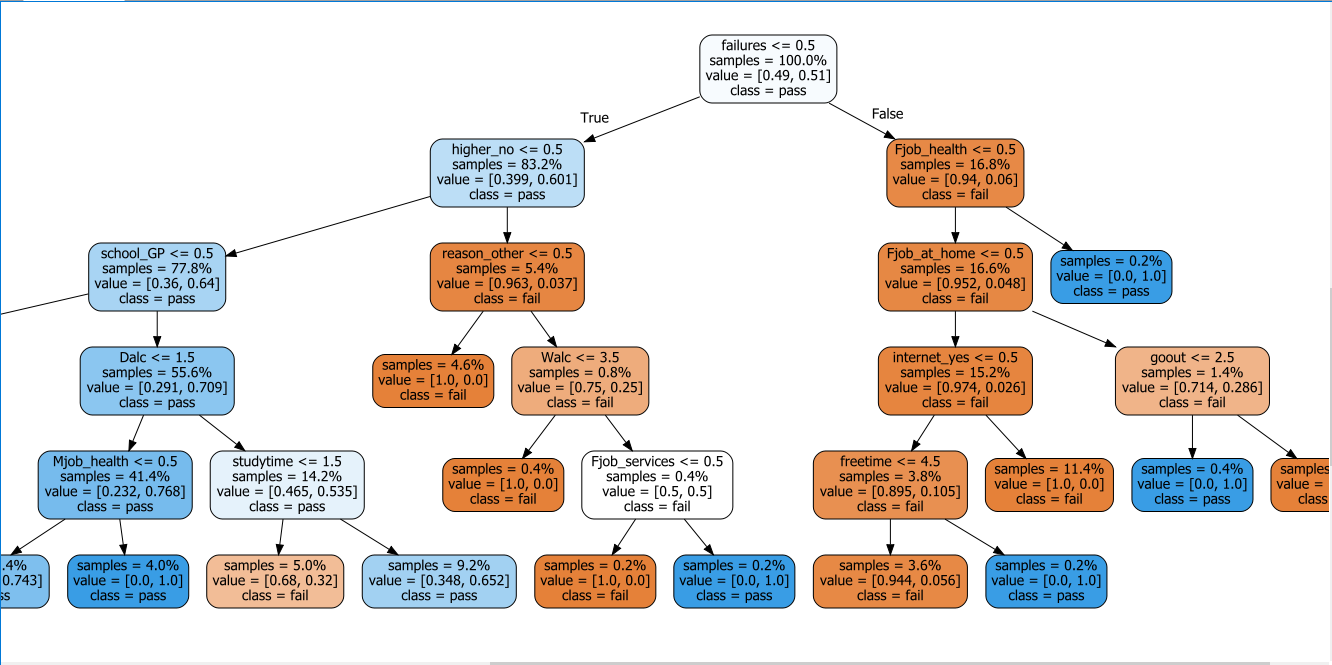
\includegraphics[width=1\textwidth]
      {figures/cokro/hasil6}}
      \caption{hasil pembuatan puhon keputusan}
      \label{hasil6}
      \end{figure}

\item selanjutnya pembuatasn method untuk menyimpan data pohon dengan menarik data langsung dari pohon keputusan di buat tadi untuk code lebih jelasnya dapat dilihat pada gambar\ref{c25}. kemudian intuk hasilnya dapat dilihat pada gambar \ref{hasil7} berikut.

\begin{figure}[ht]
      \centerline{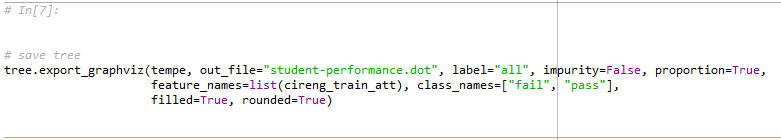
\includegraphics[width=1\textwidth]
      {figures/cokro/c25}}
      \caption{coding save}
      \label{c25}
      \end{figure}

\begin{figure}[ht]
      \centerline{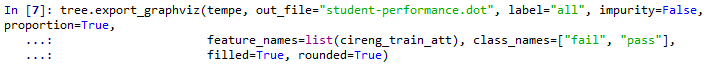
\includegraphics[width=1\textwidth]
      {figures/cokro/hasil7}}
      \caption{hasil coding save }
      \label{hasil7}
      \end{figure}

\item selanjutnya pada codingan berikut yaitu digunakan untuk mencetak nilai score rata-rata dari ketepatan data yang telah di olah tadi lebih jelsnya dapat dilihat pada gambar \ref{c26} kemudian untuk hasilnya dapat dilihat pada gambar \ref{hasil8} tersebut:

\begin{figure}[ht]
      \centerline{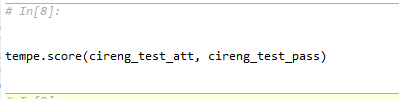
\includegraphics[width=1\textwidth]
      {figures/cokro/c26}}
      \caption{Contoh Binary Classification}
      \label{c26}
      \end{figure}

\begin{figure}[ht]
      \centerline{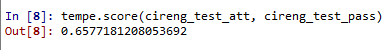
\includegraphics[width=1\textwidth]
      {figures/cokro/hasil8}}
      \caption{hasil coding save }
      \label{hasil8}
      \end{figure}

\item selanjutnya yaitu digunakan untuk memeriksa akurasi dari ketepatan hasil pengolahan data tersebut maka akan didapat nilai rata-rata 60 persen dari hasil pengolahan data tersebut untuk lebih jelasnya dapat di lihat pada gambar \ref{c27} pada codingan tersebut pada baris ke satu melakukan import library dari sklern kemudian pada baris selanjutnya mengisi nilai skor dengan nilai pada variabel tempe setelah hal tersebut dilakukan kemudian data tersebut di eksekusi. berikut merupakan hasil dari code tersebut dapat dilihat pada gambar \ref{hasil9}.

\begin{figure}[ht]
      \centerline{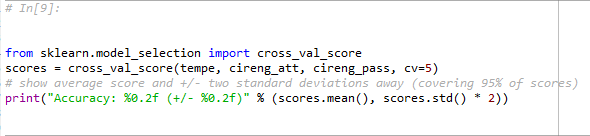
\includegraphics[width=1\textwidth]
      {figures/cokro/c27}}
      \caption{Akurasi perhitungan pohon keputusan}
      \label{c27}
      \end{figure}

\begin{figure}[ht]
      \centerline{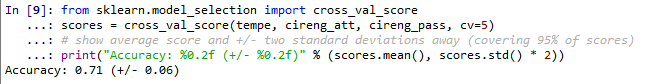
\includegraphics[width=1\textwidth]
      {figures/cokro/hasil9}}
      \caption{hasil Akurasi perhitungan pohon keputusan }
      \label{hasil9}
      \end{figure}

\item membuat rank akurasi dari 1 sampai 20 untuk melihat akurasi data apakah datatersebut terdapat di rata rata 60 persen atau tidak dengan cara membuat lagi variabel baru dengan nilai tree diadalammya jadi hampir mirip seperti membuat pohon keputusan namun ini langsung dalam bentuk rata rata akurasi yanlebih spesifik untuk lebih jelasnya dpat dilihat pada gambar\ref{c28} codingan berikut. dan untuk hasilnya dapat dilihat pada gambar \ref{hasil10} berikut.

\begin{figure}[ht]
      \centerline{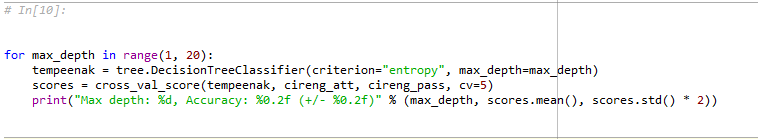
\includegraphics[width=1\textwidth]
      {figures/cokro/c28}}
      \caption{Contoh Binary Classification}
      \label{c28}
      \end{figure}

\begin{figure}[ht]
      \centerline{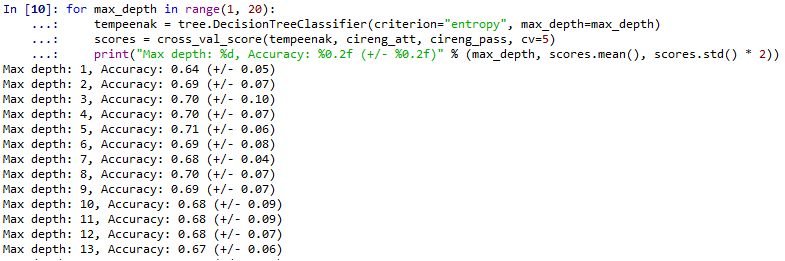
\includegraphics[width=1\textwidth]
      {figures/cokro/hasil10}}
      \caption{hasil Akurasi perhitungan pohon keputusan }
      \label{hasil10}
      \end{figure}

\item untuk selanjutnya yaitu menentukan nilai untuk grafik hampirsama dengan nilia akurasi tadi pertama tentukan rank atai batasan nilai itu disini batasannya di mulai dari 1 sampai 20 dengan menggunakan nilai tree tadi maka hasilnya dapat ditentuka kemudian buat variabel i untuk penomoran tiap record yang keluar atau recod hadil dari eksekusi tree tersebut. untuk lebih jelasnya dapat dilihat pada gambar \ref{c29} dan untuk hasilnya dapat dilihat pada gambar \ref{hasil11}.

\begin{figure}[ht]
      \centerline{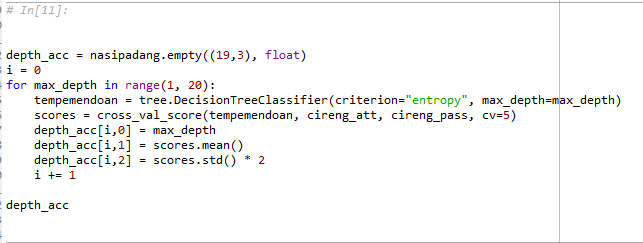
\includegraphics[width=1\textwidth]
      {figures/cokro/c29}}
      \caption{Contoh Binary Classification}
      \label{c29}
      \end{figure}

\begin{figure}[ht]
      \centerline{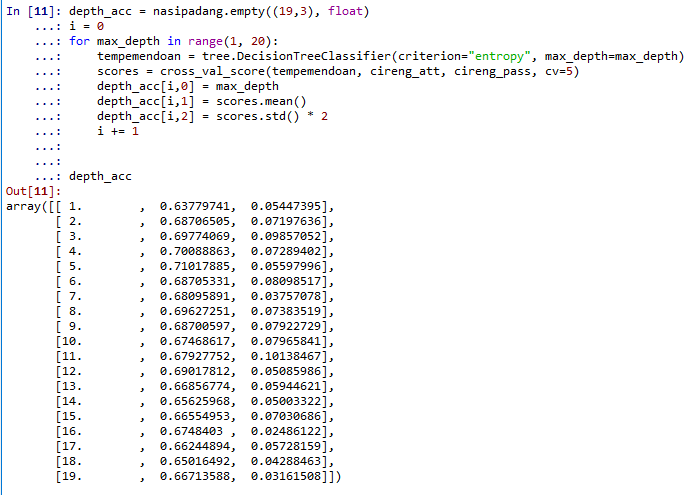
\includegraphics[width=1\textwidth]
      {figures/cokro/hasil11}}
      \caption{hasil Akurasi perhitungan pohon keputusan }
      \label{hasil11}
      \end{figure}

\item terakhir yaitu pembuatan grafik untuk pembuatan grafik diambil data dari codingan sebelumnya yang 20 record tadi dengan cara mengimport libray matplotlib.pyplot yang di inisialisasi menjadi bakwankemudian inisialisasi tersebut di eksekusi. untuk lebih jelasnya codingannya seperti gambar \ref{c30} dan untuk hasilnya seperti gambar \ref{hasil12} berikut. 

\begin{figure}[ht]
      \centerline{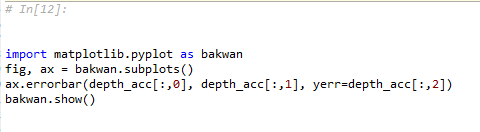
\includegraphics[width=1\textwidth]
      {figures/cokro/c30}}
      \caption{codingan pembuatan grafik}
      \label{c30}
      \end{figure}

\begin{figure}[ht]
      \centerline{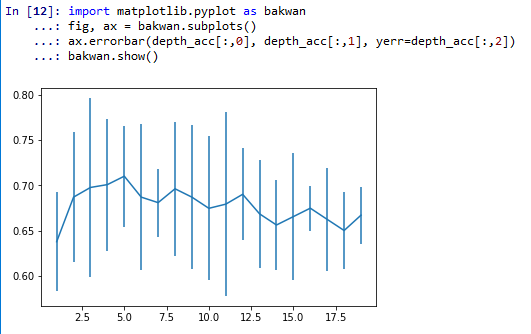
\includegraphics[width=1\textwidth]
      {figures/cokro/hasil12}}
      \caption{hasil grafik }
      \label{hasil12}
      \end{figure}
\end{enumerate}

\subsection{Penanganan Error /Cokro Edi Prawiro/1164069}
\begin{enumerate}
\item skrinsut error dapat dilihat pada gambar \ref{c31}

\begin{figure}[ht]
      \centerline{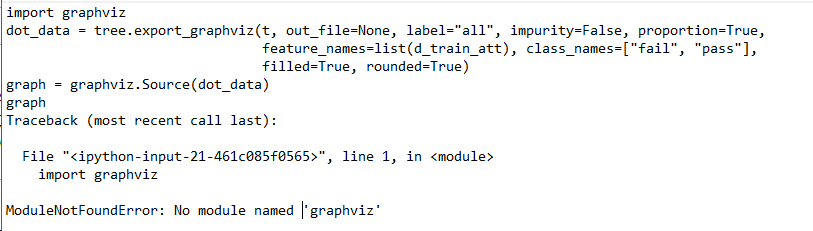
\includegraphics[width=1\textwidth]
      {figures/cokro/c31}}
      \caption{Scrensot error }
      \label{c31}
     \end{figure}

\item kode error dan jenis errornya .
\begin{verbatim}
import graphviz
dot_data = tree.export_graphviz(tempe, out_file=None, label="all", impurity=False, proportion=True,
                                feature_names=list(cireng_train_att), class_names=["fail", "pass"], 
                                filled=True, rounded=True)
graph = graphviz.Source(dot_data)
graph
\end{verbatim}

pada codingan tersebut error karena graphiznya belu di istall 

\item Solusi pemecahan masalah \par
buka CMD komputer anda run as administrator koemudian masukan perintah conda install graphviz kemudian tekan enter ingat hal ini dilakukan harus terkoneksi dengan jaringan internet. untuk hasinya dapat dilihat pada gambar\ref{c32} dan gambar \ref{c33}
setelah itu masukan PATH graphviz dengan cara masuk ke direktori graphviz itu di simpan kalau di komputer saya disempan di 
\begin{verbatim}C:\ProgramData\Anaconda3\Library\bin\graphviz \end{verbatim} kemudian setelah itu copy alamat direktori tersebut dan masukan kedalam path seperti pada gambar \ref{c34} dan pada gambar \ref{c35}.

\begin{figure}[ht]
      \centerline{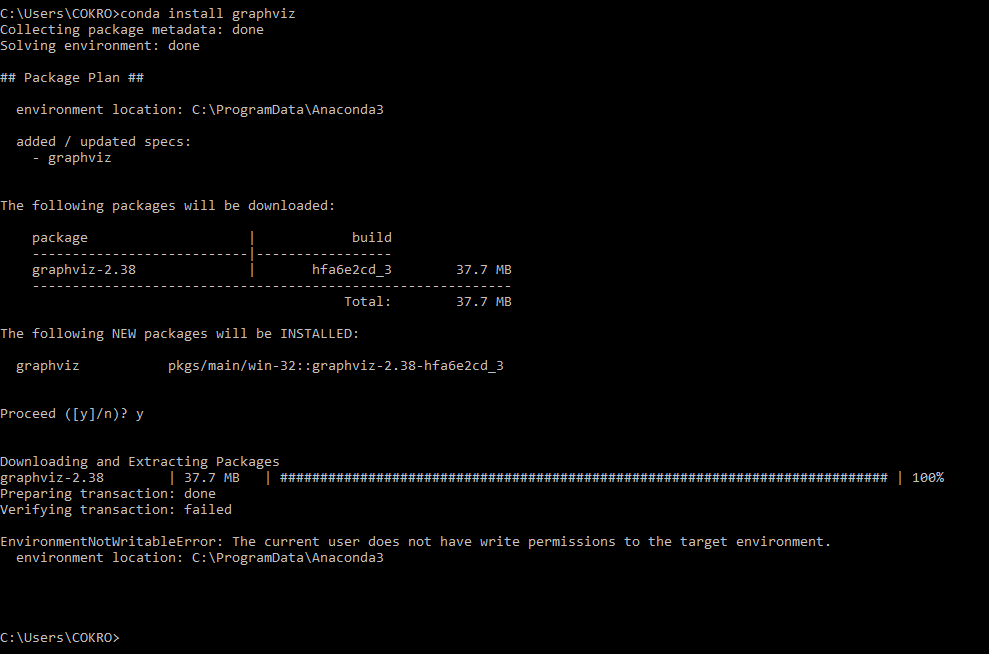
\includegraphics[width=1\textwidth]
      {figures/cokro/c32}}
      \caption{Proses instalisasi  graphviz }
      \label{c32}
     \end{figure}

\begin{figure}[ht]
      \centerline{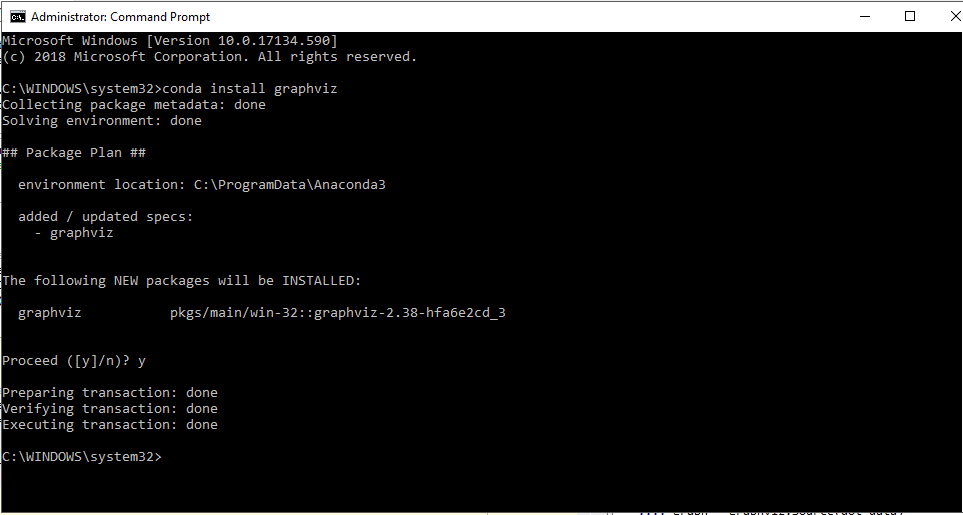
\includegraphics[width=1\textwidth]
      {figures/cokro/c33}}
      \caption{Proses instalisasi  graphviz di user }
      \label{c33}
     \end{figure}

\begin{figure}[ht]
      \centerline{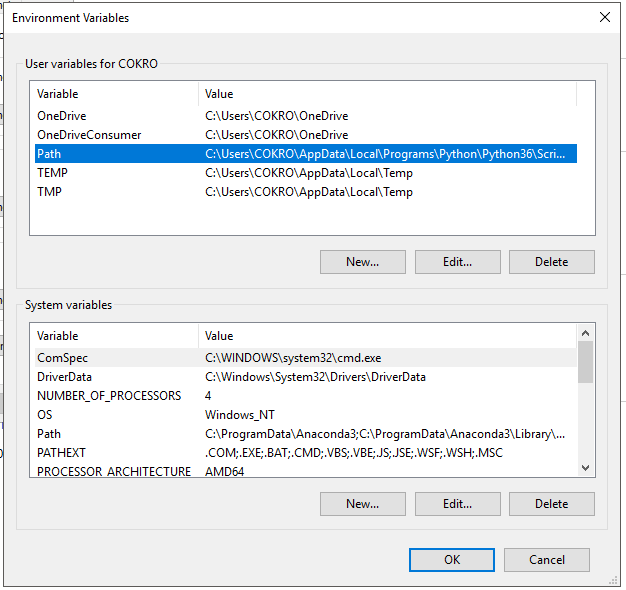
\includegraphics[width=1\textwidth]
      {figures/cokro/c34}}
      \caption{Path Komputer}
      \label{c34}
     \end{figure}

\begin{figure}[ht]
      \centerline{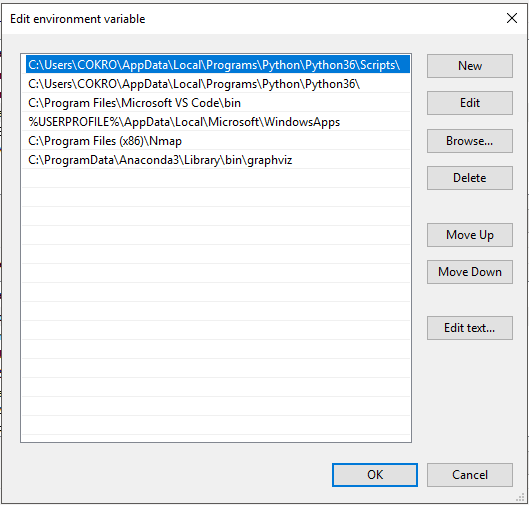
\includegraphics[width=1\textwidth]
      {figures/cokro/c35}}
      \caption{Memasukan Direktori Ke Path }
      \label{c35}
     \end{figure}


\end{enumerate}

\section{Ahmad Syafrizal Huda/1164062}
\subsection{Teori}
\begin{enumerate}
\item Binary Classification yaitu katakanlah kita memiliki tugas untuk mengklasifikasikan objek menjadi dua kelompok berdasarkan beberapa fitur. Sebagai contoh, katakanlah kita diberi beberapa pena dan pensil dari berbagai jenis dan merek, kita dapat dengan mudah memisahkannya menjadi dua kelas, yaitu pena dan pensil.
\subitem Contoh ilustrasi gambar bisa dilihat pada gambar \ref{1}.

\item Supervised learning merupakan sebuah pendekatan dimana sudah terdapat data yang dilatih, dan terdapat variable yang ditargetkan sehingga tujuan dari pendekatan ini adalah mengkelompokan suatu data ke data yang sudah ada. Sedangkan unsupervised learning tidak memiliki data latih, sehingga dari data yang ada, kita mengelompokan data tersebut menjadi 2 bagian atau 3 bagian dan seterusnya. Dan clustering adalah proses pengelompokan entitas yang sama bersama-sama. Tujuan dari teknik pembelajaran mesin tanpa pengawasan ini adalah untuk menemukan kesamaan pada titik data dan mengelompokkan titik data yang serupa secara bersamaan\cite{zhu2009introduction}.
\subitem Contoh ilustrasi gambar bisa dilihat pada gambar \ref{2}.
\subitem Contoh ilustrasi gambar bisa dilihat  pada gambar \ref{3}.
\item Evaluasi dan akurasi adalah bagaimana cara kita bisa mengevaluasi sebarapa baik model mengerjakan pekerjaannya dengan cara mengukur akurasinya. Akurasi nantinya didefinisikan sebagai presentase kasus yang telah diklasifikasikan dengan benar. Kita dapat melakukan analisis kesalahan yang telah di buat oleh model.
\subitem Contoh ilustrasi gambar bisa dilihat pada gambar \ref{5}.
\item Cara membuat dan membaca confusion matrix yaitu, menentukan pokok permasalahan serta atributnya, membuat Decision Tree, membuat Data Testing, mencari nilai variabelnya misal a,b,c, dan d, mencari nilai recall, precision, accuracy, dan erorr rate.
\subitem Contoh Confusion Matrix.
\begin{verbatim}
		Recall =3/(1+3) = 0,75
		Precision = 3/(1+3) = 0,75
		Accuracy =(5+3)/(5+1+1+3) = 0,8
		Error Rate =(1+1)/(5+1+1+3) = 0,2 
\end{verbatim}
\item Berikut ini tata cara kerja K-fold Cross Validation>
	\begin{itemize}
		\item Total instance akan dibagi menjadi N bagian.
		\item Fold yang pertama adalah bagian pertama menjadi testing data dan sisanya menjadi training data.
		\item Hitung akurasi berdasarkan porsi data tersebut dengan menggunakan persamaan.
		\item Fold yang ke dua adalah bagian ke dua menjadi testing data dan sisanya training data. 
		\item Hitung akurasi berdasarkan porsi data tersebut.
		\item Lakukan step secara berulang hingga habis mencapai fold ke-K.
		\item Terakhir hitung rata-rata akurasi K buah.
	\end{itemize}
\subitem Contoh ilustrasi gambar bisa dilihat pada gambar \ref{6}.
\item Decision Tree adalah sebuah metode pembelajaran yang digunakan untuk melakukan klarifikasi dan regresi. Decision Tree digunakan untuk membuat sebuah model yang dapat memprediksi sebuah nilai variabel target dengan cara mempelajari aturan keputusan dari fitur data. Contoh Decision Tree adalah untuk melakukan predikisi apakah Kuda termasuk hewan mamalia atau bukan.
\subitem Contoh ilustrasi gambar bisa dilihat pada gambar \ref{7}.
\item Gain adalah pengurangan yang diharapkan dalam enthropy. Dalam mechine learning, gain dapat digunakan untuk menentukan sebuah urutan atribut atau memperkecil atribut yang telah dipilih. Urutan ini akan membentuk decision tree, atribut gain dipilih yang paling besar. Dan Entropi adalah ukuran ketidakpastian sebuah variabel acak sehingga dapat di artikan entropi adalah ukuran ketidakpastian dari sebuah atribut.
\subitem Contoh ilustrasi gambar bisa dilihat pada gambar \ref{8}.
\end{enumerate}

\subsection{Scikit-learn}
\begin{enumerate}
\item Penjelasan Codingan ini akan menampilkan data pada file yang ditentukan. Untuk codingan ini file yang dieksekusi untuk digunakan ialah student-mat.csv. Secara jelasnya, dalam codingan dapat dilihat bahwa variabel buahpir didefinisikan untuk pembacaan csv dari " buahnaga  dimana untuk pemisahnya yaitu separation berupa ; . Setelah itu variabel buahpir di tampilkan dengan perintah menampilkan len panjang ataupun jumlah dan hasilnya berupa angka 395 . 
\subitem Gambar Screenshootan codingan dan hasil bisa dilihat pada gambar \ref{9}.
\begin{figure}[ht]
		\centerline{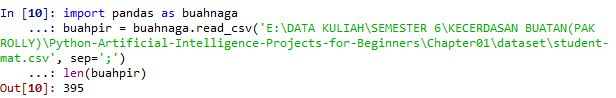
\includegraphics[width=1\textwidth]{figures/huda/1_hari4.JPG}}
		\caption{Hasil Codingan No 1.}
		\label{9}
\end{figure}
\item Penjelasan codingan ini berfungsi untuk menampilkan  baris  G1, G2 dan G3 ( berdasarkan kriterianya ) untuk kolom PASS pada variabel buahpir. Untuk lebih jelasnya, pada codingan terdapat pendefinisian pembacaan lamda ( panjang gelombang ) dari baris G1, G2 dan G3. Apabila row-row tersebut bernilai lebih dari 35 maka akan terdefinisikan angka 1 apabila tidak, maka akan terdefinisikan angka 0 pada kolom PASS ( sesuai permintaan awal ). Selanjutnya variabelnya di ditampilkan sehingga menampilkan keluaran. Tidak lupa terdapat juga jumlah dari baris dan kolom yang terubah sesuai dengan baris yang dieksekusi.
\subitem Gambar Screenshootan codingan dan hasil bisa dilihat pada gambar \ref{10}.
\begin{figure}[ht]
		\centerline{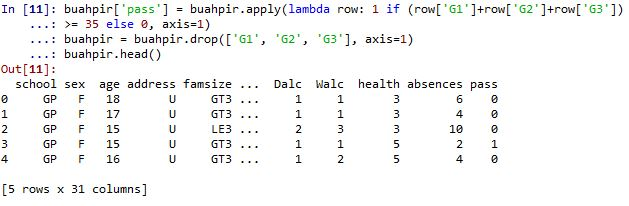
\includegraphics[width=1\textwidth]{figures/huda/2_hari4.JPG}}
		\caption{Hasil Codingan No 2.}
		\label{10}
\end{figure}
\item Penjelasan codingan ini mendefinisikan pemanggilan get dummies dari buahnaga dalam variabel buahpir. Di dalam get dummies sendiri akan terdefinisikan variabel buahpir dengan kolom-kolom yang akan dieksekusi seperti school, address dll. Kemudian variabel tersebut diartikan untuk mendapatkan kembalian berupa keluaran dari eksekusi perintah variabel buahpir beserta dengan jumlah baris dan kolom data yang dieksekusi.
\subitem Gambar Screenshootan codingan dan hasil bisa dilihat pada gambar \ref{11}.
\begin{figure}[ht]
		\centerline{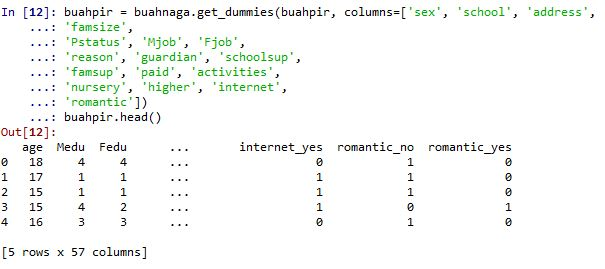
\includegraphics[width=1\textwidth]{figures/huda/3_hari4.JPG}}
		\caption{Hasil Codingan No 3.}
		\label{11}
\end{figure}
\item Penjelasan codingan ini difungsikan untuk mengartikan pembagian data yang berupa training dan testing data. pertama-tama variabel buahpir akan mengartikan sampel yang akan digunakan ( berupa shuffle row ) . Nah kemudian masing-masing parameter yaitu buahpir train dan buahpir test akan berjumlah 500 data ( telah dibagi untuk training dan testing ). Selanjutnya dilakukan pengeksekusian untuk kolom Pass, apabila sesuai dengan axis=1 maka eksekusi fungsi berhasil. Selain itu juga disertakan jumlah dari peserta yang lolos dari semua nilai data setnya.  
\subitem Gambar Screenshootan codingan dan hasil bisa dilihat pada gambar \ref{12}.
\begin{figure}[ht]
		\centerline{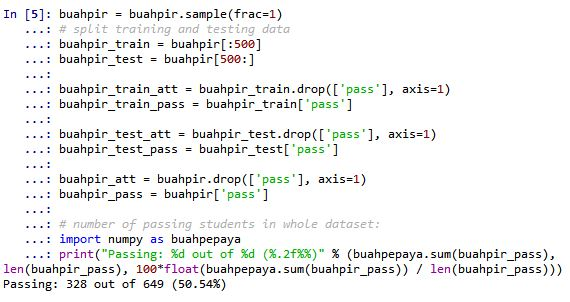
\includegraphics[width=1\textwidth]{figures/huda/4_hari4.JPG}}
		\caption{Hasil Codingan No 4.}
		\label{12}
\end{figure}
\item Penjelasan codingan ini hanya membuktikan pengujian dari Klasifikasi Decision Tree yang ada, apakah true atau tidak dan hasilnya true. Pada codingan ini di definisikan library sklearn untuk mengimpot atau menampilkan tree. Variabel buahapel difungsikan untuk membaca klasifikasi decision tree dari tree itu sendiri dengan 2 parameternya yaitu kriteria=entropy dan max depth=5. Maka selanjutnya variabel buahapel akan masuk dan terbaca dalam module fit dengan 2 parameter yaitu buahpir trai att dan buahpir train pass.
\subitem Gambar Screenshootan codingan dan hasil bisa dilihat pada gambar \ref{13}.
\begin{figure}[ht]
		\centerline{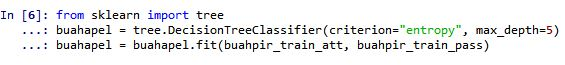
\includegraphics[width=1\textwidth]{figures/huda/5_hari4.JPG}}
		\caption{Hasil Codingan No 5.}
		\label{13}
\end{figure}
\item Penjelasan codingan ini memberikan gambaran dari klasifikasi decision tree yaitu pengolahan parameter yang dieksekusi kedalam variabel buahapel. Tentunya dengan pemanfaatan library graphviz yang telah diimport dan difungsikan.
\subitem Gambar Screenshootan codingan dan hasil bisa dilihat pada gambar \ref{14}.
\begin{figure}[ht]
		\centerline{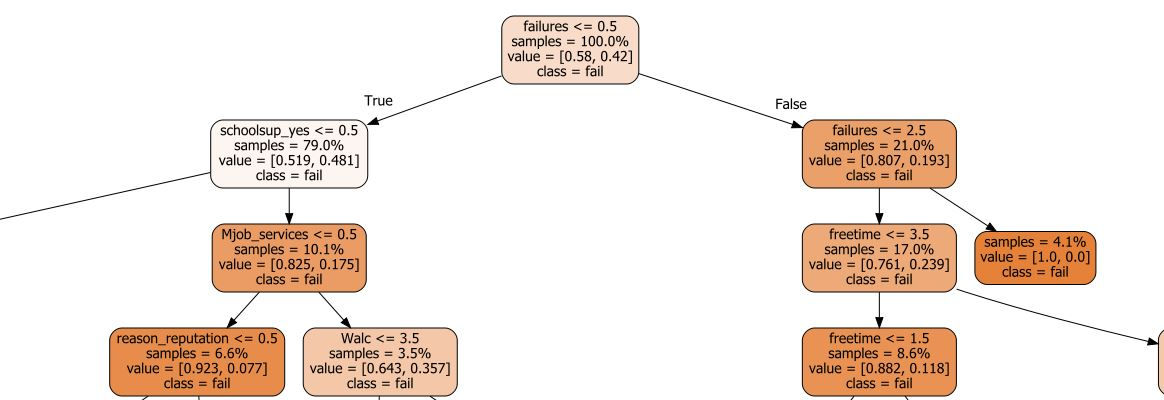
\includegraphics[width=1\textwidth]{figures/huda/6_hari4.JPG}}
		\caption{Hasil Codingan No 6.}
		\label{14}
\end{figure}
\item Penjelasan codingan ini membahas tentang penyimpanan tree dari library graphviz yang dieksekusi bersamaan dengan variabel buahapel dan parameter lainnya. Dilakukan pengecekan dan pengujian apakah klasifikasi decision treenya dapat berjalan atau tidak. Apabila tidak berjalan, maka akan terjadi error, namun codingan ini berfungsi.
\subitem Gambar Screenshootan codingan dan hasil bisa dilihat pada gambar \ref{15}.
\begin{figure}[ht]
		\centerline{\includegraphics[width=1\textwidth]{figures/huda/7_hari4.JPG}}
		\caption{Hasil Codingan No 7.}
		\label{15}
\end{figure}
\item Penjelasan codingan ini membaca score dari variabel buahapel dimana terdapat 2 parameter yang dihitung dan diuji yaitu buahpir test att dan buahpir test pass. Untuk hasilnya sendiri mengapa berupa angka, dikarenakan pada parameter yang dieksekusi memang memiliki data sehingga dieksekusi dan menghasilkan keluaran dari score tersebut.
\subitem Gambar Screenshootan codingan dan hasil bisa dilihat pada gambar \ref{16}.
\begin{figure}[ht]
		\centerline{\includegraphics[width=1\textwidth]{figures/huda/8_hari4.JPG}}
		\caption{Hasil Codingan No 8.}
		\label{16}
\end{figure}
\item Penjelasan codingan ini membahas mengenai pengkesekusian fungsi dan variabel dari library yang didefinisikan dan yang diimport. Penjelasan lebih jelasnya ialah codingan ini mendefinisikan library sklearn.model.selection kemudian mengimport cross val score. Kemudian variabel score mendefinisikan cross val score yang telah diimport tadi dengan 4 parameter yaitu buahapel, buahpir att, buahpir pass dan cv=5 untuk dieksekusi. Setelah semua pemrosesan tersebut maka hasil yang di tampilkan ialah rata2 perhitungan dari variabel score dimana dan standar dari plus minusnya tentunya dengan ketentuan parameter Accuracy .
\subitem Gambar Screenshootan codingan dan hasil bisa dilihat pada gambar \ref{17}.
\begin{figure}[ht]
		\centerline{\includegraphics[width=1\textwidth]{figures/huda/9_hari4.JPG}}
		\caption{Hasil Codingan No 9.}
		\label{17}
\end{figure}
\item Penjelasan Codingan ini mendefinisikan max depth dalam jarak angka antara parameter 1 dan 20. Variabel buahapel mendefinisikan klasifikasi decision tree dengan 2 parameter. Kemudian variabel score mengeksekusi parameter lainnya yaitu seperti buahapel, buahpir att, buahpir pass dan cv=5 ) . Hasil yang ditampilkan ialah dari max depth, accuracy dan plus minusnya dan akhirnya hasil outputannya keluar.
\subitem Gambar Screenshootan codingan dan hasil bisa dilihat pada gambar \ref{18}.
\begin{figure}[ht]
		\centerline{\includegraphics[width=1\textwidth]{figures/huda/10_hari4.JPG}}
		\caption{Hasil Codingan No 10.}
		\label{18}
\end{figure}
\item Penjelasan codingan ini mengartikan bahwa variabel depth\_acc akan mengeksekusi empty dari importan library numphy yang dinamakan buahpepaya dengan 2 parameter yaitu 19,3 dan float. i didefinisikan dengan angka 0 kemudian untuk perhitungan jarak max depth diantara parameter 1 dan 20. Variabel buahapel mengartikan klasifikasi decision tree dengan 2 parameter. setelah itu, variabel score mendefinisikan variabel depth\_acc dengan i dan 0, variabel kedua dari depth\_acc dengan i dan 1 serta variabel ketiga dari depth\_acc dengan i dan 2, maka pengeksekusian akhir bahwa variabel i akan ditambah dengan angka 1 untuk hasil akhirnya. Keluarannya akan berupa array dari perhitungan parameter dan variabel yang telah didefinisikan sebelumnya.
\subitem Gambar Screenshootan codingan dan hasil bisa dilihat pada gambar \ref{19}.
\begin{figure}[ht]
		\centerline{\includegraphics[width=1\textwidth]{figures/huda/11_hari4.JPG}}
		\caption{Hasil Codingan No 11.}
		\label{19}
\end{figure}
\item Penjelasan codingan ini mendefinisikan pemanggilan dari library matplotlib.pyplot sebagai buahanggur sehingga nanti hasilnya akan berbentuk gambar grafik/gelombang. Untuk variabel fig dan ax akan mendefinisikan subplots dari buahanggur. Setelah itu ketentuan dari parameter depth acc = 0, depth acc = 1 dan depth acc 2. Selanjutnya untuk menampilkan gelombang maka panggil variabel buahanggur dengan perintah show.
\subitem Gambar Screenshootan codingan dan hasil bisa dilihat pada gambar \ref{20}.
\begin{figure}[ht]
		\centerline{\includegraphics[width=1\textwidth]{figures/huda/12_hari4.JPG}}
		\caption{Hasil Codingan No 12.}
		\label{20}
\end{figure}
\end{enumerate}

\subsection{Penanganan Eror}
\begin{enumerate}
\item ScreeShootan Eror pada codingan No 8 dapat dilihat pada gambar \ref{21}.
\subitem 
\begin{figure}[ht]
		\centerline{\includegraphics[width=1\textwidth]{figures/huda/eror6.JPG}}
		\caption{Hasil Gambar Eror No 6.}
		\label{21}
\end{figure}
\item Codingan eror dan jenis erornya : sebenarnya tidak terdapat eror pada codingan ini namun saat pertama kali di run current cell codingan ini akan eror dan tidak keluar outputannya dikarenakan library graphviz sebelumnya tidak ditemukan atau belum di install terlebih dahulu.
\subitem 
\begin{verbatim}
import graphviz
dot_data = tree.export_graphviz(buahapel, out_file=None, label="all", impurity=False, proportion=True,
                                feature_names=list(buahpir_train_att), class_names=["fail", "pass"], 
                                filled=True, rounded=True)
graph = graphviz.Source(dot_data)
graph
\end{verbatim}
\item Solusi pemecahan masalah eror tersebut yaitu dengan cara menginstall terlebih dahulu library graphviznya pada anaconda prompt atau command prompt anda dengan perintah conda install graphviz setelah itu run kembali codingan No 8 maka akan muncul outputan atau tampilan keluarannya.
\subitem Berikut gambar cara menginstall graphviz dapat dilihat pada gambar \ref{22}
\begin{figure}[ht]
		\centerline{\includegraphics[width=1\textwidth]{figures/huda/penangananeror6.JPG}}
		\caption{Hasil Gambar Penanganan Eror No 6.}
		\label{22}
\end{figure}
\end{enumerate}


\begin{figure}[ht]
		\centerline{\includegraphics[width=1\textwidth]{figures/huda/binary.JPG}}
		\caption{Binary Classification.}
		\label{1}
\end{figure}
\begin{figure}[ht]
		\centerline{\includegraphics[width=1\textwidth]{figures/huda/supervised.JPG}}
		\caption{Supervised Learning.}
		\label{2}
\end{figure}
\begin{figure}[ht]
		\centerline{\includegraphics[width=1\textwidth]{figures/huda/unsupervised.JPG}}
		\caption{Unsupervised Learning.}
		\label{3}
\end{figure}
\subitem Contoh ilustrasi gambar bisa dilihat pada gambar \ref{4}.
\begin{figure}[ht]
		\centerline{\includegraphics[width=1\textwidth]{figures/huda/clustering.JPG}}
		\caption{Clustering.}
		\label{4}
\end{figure}
\begin{figure}[ht]
		\centerline{\includegraphics[width=1\textwidth]{figures/huda/evaluasidanakurasi.JPG}}
		\caption{Evaluasi dan Akurasi.}
		\label{5}
\end{figure}
\begin{figure}[ht]
		\centerline{\includegraphics[width=1\textwidth]{figures/huda/K-fold.JPG}}
		\caption{K-fold Cross Validation.}
		\label{6}
\end{figure}
\begin{figure}[ht]
		\centerline{\includegraphics[width=1\textwidth]{figures/huda/DecisionTree.JPG}}
		\caption{Decision Tree.}
		\label{7}
\end{figure}
\begin{figure}[ht]
		\centerline{\includegraphics[width=1\textwidth]{figures/huda/Gain.PNG}}
		\caption{Gain.}
		\label{8}
\end{figure}

\begin{figure}[ht]
      \centerline{\includegraphics[width=1\textwidth]
      {figures/c10}}
      \caption{Contoh Binary Classification}
      \label{c10}
      \end{figure}

\begin{figure}[ht]
      \centerline{\includegraphics[width=1\textwidth]
      {figures/c11}}
      \caption{Ilustrasi Suvervised Learning}
      \label{c11}
      \end{figure}

\begin{figure}[ht]
      \centerline{\includegraphics[width=1\textwidth]
      {figures/c12}}
      \caption{Ilustrasi Unsuvervised Learning}
      \label{c12}
      \end{figure}

\begin{figure}[ht]
      \centerline{\includegraphics[width=1\textwidth]
      {figures/c13}}
      \caption{Ilustrasi Clustering}
      \label{c13}
      \end{figure}

\begin{figure}[ht]
      \centerline{\includegraphics[width=1\textwidth]
      {figures/c14}}
      \caption{Ilustrasi Evaluasi}
      \label{c14}
      \end{figure}

\begin{figure}[ht]
      \centerline{\includegraphics[width=1\textwidth]
      {figures/c15}}
      \caption{Ilustrasi Confusion Matrix}
      \label{c15}
      \end{figure}

\begin{figure}[ht]
      \centerline{\includegraphics[width=1\textwidth]
      {figures/c16}}
      \caption{Ilustrasi K-Fold}
      \label{c16}
      \end{figure}

\begin{figure}[ht]
      \centerline{\includegraphics[width=1\textwidth]
      {figures/c17}}
      \caption{Ilustrasi Decision Tree}
      \label{c17}
      \end{figure}

\begin{figure}[ht]
      \centerline{\includegraphics[width=1\textwidth]
      {figures/c18}}
      \caption{Contoh Ilustrasi Information Gain.}
      \label{c18}
      \end{figure}

\section{Fathi Rabbani / 1164074}
\subsection{Teori}
\begin{enumerate}

\item Binary Classification
\subitem
membuat sebuah klasifikasi dengan menggunakan 2 buah hasil data yang menghasilkan himpunan data dalam dua kelompok yang berbeda. berikut adalah contohnya \ref{a1}.
\begin{figure}
\centerline{\includegraphics[width=1\textwidth]{figures/fathi/chapter2/1.PNG}}
\caption{Contoh Penggunaan Binary Classification}
\label{a1}
\end{figure}

\item Supervised, Unsupervised and Clustering
\begin{itemize}
\item Supervised Learning
supervised learning adalah cara untuk mengklasifikasikan suatu objek atau data yang telah di tentukan kelasnya, berikut adalah contohnya \ref{a2}.
\item Unsupervised Learning
unsupervised learning merupakan cara untuk mengklasifikasi tanpa adanya kelas untuk menentukan jenis datanya, berikut ini contohnya \ref{a3}.
\item Clustering
clustering merupakan peroses mengklasifikasikan yang berdasarkan suatu parameter dalam penentuan hasilnya, berikut contohnya \ref{a4}
\end{itemize}

\begin{figure}
\centerline{\includegraphics[width=1\textwidth]{figures/fathi/chapter2/2.PNG}}
\caption{Contoh Penggunaan Supervised Learning}
\label{a2}

\centerline{\includegraphics[width=1\textwidth]{figures/fathi/chapter2/3.PNG}}
\caption{Contoh Penggunaan Unsupervised Learning}
\label{a3}

\centerline{\includegraphics[width=1\textwidth]{figures/fathi/chapter2/4.PNG}}
\caption{Contoh Penggunaan Clustering}
\label{a4}
\end{figure}

\item Evaluasi dan Akurasi
\begin{itemize}
\item Evaluasi
evaluasi adalah sebuah proses dalam mengumpulkan serta mengamati bukti untuk mengukur dampak dari suatu objek, data, program atau proses yang berkaitan itu sendiri, berikut contohnya \ref{a5}.
\item Akurasi
akurasi merupakan ketepatan dalam sebuah proses dalam melakukan perhitungan akan proses yang sedang berlangsung.
\end{itemize}

\begin{figure}
\centerline{\includegraphics[width=1\textwidth]{figures/fathi/chapter2/5.PNG}}
\caption{Contoh Penggunaan Evaluasi dan Akurasi}
\label{a5}
\end{figure}

\item Membuat dan Membaca Confusion Matrix
menentukan objek yang digunakan sebagai bahan uji, sebagai contoh usia 20, 30 dan 40 dengan membuat sebuah tabel yang dapat menampung data dengan nilai 10 pada gambar \ref{a6} . lalu data tersebut bisa juga berupa data sebagai berikut \ref{a7}.
membaca data Matrix tersebut dengan mengunakan Usia sebagai data standarnya dengan rentang usia 20 hingga 40 tahun, lalu jumlah orang yang dapat di ketahui adalah 10 dan data yang ternilai haruslah berisi 10 agar data tersebut valid.

\begin{figure}
\centerline{\includegraphics[width=1\textwidth]{figures/fathi/chapter2/6.PNG}}
\caption{Contoh Matrix Confusion}
\label{a6}

\centerline{\includegraphics[width=1\textwidth]{figures/fathi/chapter2/7.PNG}}
\caption{Contoh Matrix Confusion}
\label{a7}
\end{figure}

\item K-Fold Cross Validation
K-fold Cross Validation merupakan cara untuk melatih suatu mesin dimana di dalammya terdapat data set yang dibagi menjadi dua yaitu untuk data testing dan data training contoh 100 datasebesar 20 data digunakan untuk data testing kemudian 80 datanya digunakan untuk data training dimana data training tersebut digunakan untuk menentukan nilai bobot yang dimasukan kedalam rumus regresi linier. seperti berikut \ref{a8}.

\begin{figure}
\centerline{\includegraphics[width=1\textwidth]{figures/fathi/chapter2/8.PNG}}
\caption{Contoh Penggunaan K Fold Cross Validation}
\label{a8}
\end{figure}

\item Decision Tree
merupakan implementasi dari binari clasification dimana  akan terdapat  akar dan cabang data yang memiliki nilai if...else contoh pada akar data berisi nilai jenis kelamin, apakah pria pada cabang satu bernilai iya dan pada cabang dua bernilai tidak jika nilainya iya berarti jenis kelaminya pria dan jika tidak maka bernilai wanita,  lebih jelasnya dapat dilihat pada gambar\ref{a9}.

\begin{figure}
\centerline{\includegraphics[width=1\textwidth]{figures/fathi/chapter2/9.PNG}}
\caption{Contoh Penggunaan Decision Tree}
\label{a9}
\end{figure}

\item Information Gain dan Entropi
informasion gain proses dengan mempraktekkan sistem decision tree menggunakan prinsip if...else yang berlangsung hingga menghasilkan data yang diinginkan. untuk contohnya seperti berikut ini 
sedangkan entropi merupakan ukuran keacakan dari informasi. semakin tinggi entropi maka semakin sulit dalam menentukan keputusan, berikut contohnya \ref{a10}.

\begin{figure}
\centerline{\includegraphics[width=1\textwidth]{figures/fathi/chapter2/10.PNG}}
\caption{Contoh Penggunaan Information Gain}
\label{a10}
\end{figure}

\end{enumerate}

\subsection {Praktek}
\begin{itemize}
\item Code
\begin{enumerate}
\item
\begin{verbatim}
import pandas as plum
durian = plum.read_csv('dataset/student-mat.csv', sep=';')
len(durian)
\end{verbatim}
\subitem
pada code berikut menjelaskan data dari pandas dengan menggunakan nama alias plum yang akan membaca data student-mat.csv yang berada pada folder dataset. hasilnya terdapat pada gambar \ref{a11}
\item
\begin{verbatim}
durian['pass'] = durian.apply(lambda row: 1 if (row['G1']+row['G2']+row['G3']) >= 35 else 0, axis=1)
durian = durian.drop(['G1', 'G2', 'G3'], axis=1)
durian.head()
\end{verbatim}
\subitem
pada code berikut ini menjelaskan bahwa slot data pada student-mat.csv akan ditambah dengan kolom pass dan menggunakan proses lambda yang akan menghasilkan data berupa array dengan struktur G1, G2 dan G3. hasilnya bisa dilihat pada gambar \ref{a12}
\item 
\begin{verbatim}
durian = plum.get_dummies(durian, columns=['sex', 'school', 'address', 'famsize', 'Pstatus', 'Mjob', 'Fjob', 
                               'reason', 'guardian', 'schoolsup', 'famsup', 'paid', 'activities',
                               'nursery', 'higher', 'internet', 'romantic'])
durian.head()

\end{verbatim}
\subitem
pada code berikut menerangkan bahwa variable durian memiliki proses yang akan memanggil variable plum untuk mendapatkan data pada kolom tersebut. hasilnya adalah \ref{a13}
\item
\begin{verbatim}
durian = durian.sample(frac=1)
# split training and testing data
d_train = durian[:500]
d_test = durian[500:]

d_train_att = d_train.drop(['pass'], axis=1)
d_train_pass = d_train['pass']

d_test_att = d_test.drop(['pass'], axis=1)
d_test_pass = d_test['pass']

d_att = durian.drop(['pass'], axis=1)
d_pass = durian['pass']

# number of passing students in whole dataset:
import numpy as nanas
print("Passing: %d out of %d (%.2f%%)" % (nanas.sum(d_pass), len(d_pass), 100*float(nanas.sum(d_pass)) / len(d_pass)))

\end{verbatim}
\subitem
code berikut menjelaskan bahwa data durian akan diproses untuk didapatkan hasil dari penggunaan k-fold cross yang membagi data dengan training dan testing dengan hasilnya adalah seperti pada gambar \ref{a14}
\item 
\begin{verbatim}
from sklearn import tree
tomat = tree.DecisionTreeClassifier(criterion="entropy", max_depth=5)
tomat = tomat.fit(d_train_att, d_train_pass)

\end{verbatim}
\subitem
code ini mengambil data dari sklearn berupa data tree dengan variable tomat yang menampung data proses penggunaan decisiontree dan di proses dengan menggunakan data d\_train\_att dan d\_train\_pass hasilnya ada digambar \ref{a15}
\item
\begin{verbatim}
import graphviz
dot_data = tree.export_graphviz(tomat, out_file=None, label="all", impurity=False, proportion=True,
                                feature_names=list(d_train_att), class_names=["fail", "pass"], 
                                filled=True, rounded=True)
graph = graphviz.Source(dot_data)
graph
\end{verbatim}
\subitem
pada code berikut menjelaskan data graphviz yang diambli untuk menampilkan data \ref{a16}
\item 
\begin{verbatim}
tree.export_graphviz(tomat, out_file="student-performance.dot", label="all", impurity=False, proportion=True,
                     feature_names=list(d_train_att), class_names=["fail", "pass"], 
                     filled=True, rounded=True)
\end{verbatim}
\subitem
pada code ini digunakan untuk memproses data pada code 6 yang akan menghasilkan sebuah file bernama student-performance.dot hasilnya ada pada gambar \ref{a17}
\item 
\begin{verbatim}
tomat.score(d_test_att, d_test_pass)

\end{verbatim}
\subitem
pada code ini dihasilkan data seperti berikut \ref{a18} yang artinya adalah data score dari d\_test\_att dan d\_test\_pass 
\item 
\begin{verbatim}
from sklearn.model_selection import cross_val_score
apel = cross_val_score(tomat, d_att, d_pass, cv=5)

print("Accuracy: %0.2f (+/- %0.2f)" % (apel.mean(), apel.std() * 2))

\end{verbatim}
\subitem
mengambil data dari sklearn.model\_selection dan mengambil data cross\_val\_score yang digunakan untuk menghitung data akurasi dari code 5 hasilnya ada digambar \ref{a19}
\item
\begin{verbatim}
for max_depth in range(1, 20):
    tomat = tree.DecisionTreeClassifier(criterion="entropy", max_depth=max_depth)
    apel = cross_val_score(tomat, d_att, d_pass, cv=5)
    print("Max depth: %d, Accuracy: %0.2f (+/- %0.2f)" % (max_depth, apel.mean(), apel.std() * 2))

\end{verbatim}
\subitem
code ini menjelaskan hasil dari akurasi pada code 9 yang dibreakdown untuk tampil sebagai data yang terhitung seperti pada gambar \ref{a20}
\item
\begin{verbatim}
semangka = nanas.empty((19,3), float)
i = 0
for max_depth in range(1, 20):
    tomat = tree.DecisionTreeClassifier(criterion="entropy", max_depth=max_depth)
    apel = cross_val_score(tomat, d_att, d_pass, cv=5)
    semangka[i,0] = max_depth
    semangka[i,1] = apel.mean()
    semangka[i,2] = apel.std() * 2
    i += 1
    
semangka
\end{verbatim}
\subitem
pada code ini data pada code 10 di ubah menjadi seurutan array yang ada pada gambar \ref{a21}
\item 
\begin{verbatim}
import matplotlib.pyplot as melon
fig, ax = melon.subplots()
ax.errorbar(semangka[:,0], semangka[:,1], yerr=semangka[:,2])
melon.show()
\end{verbatim}
\subitem
code ini menampilkan data grafik yang digunakan untuk melihat data pada code sebelumnya hasilnya adalah seperti pada gambar \ref{a22}
\end{enumerate}
\item Hasil

\begin{figure}
\centerline{\includegraphics[width=1\textwidth]{figures/fathi/chapter2/chapter3/1.PNG}}
\caption{code 1 hasil}
\label{a11}
\end{figure}

\begin{figure}
\centerline{\includegraphics[width=1\textwidth]{figures/fathi/chapter2/chapter3/2.PNG}}
\caption{code 2 hasil}
\label{a12}
\end{figure}

\begin{figure}
\centerline{\includegraphics[width=1\textwidth]{figures/fathi/chapter2/chapter3/3.PNG}}
\caption{code 3 hasil}
\label{a13}
\end{figure}

\begin{figure}
\centerline{\includegraphics[width=1\textwidth]{figures/fathi/chapter2/chapter3/4.PNG}}
\caption{code 4 hasil}
\label{a14}
\end{figure}

\begin{figure}
\centerline{\includegraphics[width=1\textwidth]{figures/fathi/chapter2/chapter3/5.PNG}}
\caption{code 5 hasil}
\label{a15}
\end{figure}

\begin{figure}
\centerline{\includegraphics[width=1\textwidth]{figures/fathi/chapter2/chapter3/6.PNG}}
\caption{code 6 hasil}
\label{a16}
\end{figure}

\begin{figure}
\centerline{\includegraphics[width=1\textwidth]{figures/fathi/chapter2/chapter3/7.PNG}}
\caption{code 7 hasil}
\label{a17}
\end{figure}


\begin{figure}
\centerline{\includegraphics[width=1\textwidth]{figures/fathi/chapter2/chapter3/8.PNG}}
\caption{code 8 hasil}
\label{a18}
\end{figure}

\begin{figure}
\centerline{\includegraphics[width=1\textwidth]{figures/fathi/chapter2/chapter3/9.PNG}}
\caption{code 9 hasil}
\label{a19}
\end{figure}

\begin{figure}
\centerline{\includegraphics[width=1\textwidth]{figures/fathi/chapter2/chapter3/10.PNG}}
\caption{code 10 hasil}
\label{a20}
\end{figure}

\begin{figure}
\centerline{\includegraphics[width=1\textwidth]{figures/fathi/chapter2/chapter3/11.PNG}}
\caption{code 11 hasil}
\label{a21}
\end{figure}

\begin{figure}
\centerline{\includegraphics[width=1\textwidth]{figures/fathi/chapter2/chapter3/12.PNG}}
\caption{code 12 hasil}
\label{a22}
\end{figure}

\end{itemize}

\subsection {Penanganan Error}
\begin{itemize}
\item Error Path
\subitem
cara membenarkan error yang terdapat pada gambar \ref{a23} adalah dengan menginstall ulang graphviz dengan format 
\begin{verbatim}
conda install graphviz

atau

pip install graphviz
\end{verbatim}
yang terdapat pada gambar \ref{a24}
\end{itemize}

\begin{figure}
\centerline{\includegraphics[width=1\textwidth]{figures/fathi/chapter2/chapter3/21.PNG}}
\caption{Error Path}
\label{a23}
\end{figure}

\begin{figure}
\centerline{\includegraphics[width=1\textwidth]{figures/fathi/chapter2/chapter3/22.PNG}}
\caption{Fix Error}
\label{a24}
\end{figure}


 
\chapter{Methods}
\maxdeadcycles=200

\section{Fathi Rabbani / 1164074}
\subsection{Teori}
\begin{enumerate}
\item Random Forest
\subitem
Random forest  adalah suatu algoritma yang digunakan pada klasifikasi data dalam jumlah yang besar. Klasifikasi random forest dilakukan melalui penggabungan pohon (tree) dengan melakukan training pada sampel data yang dimiliki. Penggunaan pohon (tree) yang semakin banyak akan mempengaruhi akurasi yang akan didapatkan menjadi lebih baik. Penentuan klasifikasi dengan random forest diambil berdasarkan hasil voting dari tree yang terbentuk. Pemenang dari tree yang terbentuk ditentukan dengan vote terbanyak. berikut adalah struktur dari Random Forest ada pada Gambar \ref{fig1}

\item Membaca Dataset, Makna setiap file dan Menjelaskan data CUB-200-2011
\begin{enumerate}
\item Membaca Data
\begin{itemize}
\item
dengan membuka data yang sudah didownload yaitu data CUB-200-2011 atau data tentang perbandingan data jenis burung,
\item
lalu data tersebut dibuka dengan menggunakan aplikasi Spyder, dan dijalankan setiap baris Code yang ada.
\item data yang ada pada folder CUB-200-2011 dibuka dengan menggunakan code dari Chapter 2 yang ada pada buku pembelajaran.
\end{itemize}

\item Makna setiap File
\begin{itemize}
\item data yang terdapat pada file CUB-200-2011 ada data folder ATTRIBUTE, IMAGES, PARTS yang memiliki kegunaannya sendiri yang dimana pada penggunaannya data yang dipakai adalah data image\_attribute\_label pada folder attribute, data image\_class\_labels dan data classes.
\item file image\_attribute\_label berguna sebagai data awal yang digunakan untuk membaca data attribute yang terdapat pada masing - masing gambar burung yang ada.
\item sedangkan file image\_class\_label yang ada pada folder CUB-200-2011 berguna sebagai data yang akan membuat kolom baru pada dataset yang fungsinya adalah untuk memasukan hasil dari semua data yang dimiliki oleh imgatt2.
\item dan file classes berguna sebagai dataset yang akan dipanggil oleh fungsi code untuk menampilkan nama dari data burung yang dimiliki.
\end{itemize}

\item Isi Field
\begin{itemize}
\item file image\_attribute\_label
berisi tentang data attribute yang ada pada data gambar file burung yang dimiliki difolder image pada CUB-200-2011
\item file image\_class\_label
berisi tentang data yang dimiliki oleh attribute dari image\_attribute\_label dimana data yang bernilai atau memiliki nilai disusun hingga menghasilkan data yang mudah dipahami.
\item file classes
berisi tentang data yang berguna untuk menampilkan data nama dari setiap data jenis burung yang dimiliki.
\end{itemize}
\end{enumerate}

\item Cross Validation
\subitem
Cross-validation adalah metode statistik yang dapat digunakan untuk mengevaluasi kinerja model atau algoritma dimana data dipisahkan menjadi dua subset yaitu data training dan data testing.

\item Score 44 Random Forest, 27 Decision Tree dan 29 SVM
\begin{enumerate}
\item
merupakan hasil dari pengolahan tentang data jenis burung yang dimiliki setelah melalui proses pembagian data training dan testing yang menghasilkan score 44 persen sebagai pembanding bahwa data yang diolah tersebut bernilai 44 persen tingkat kebenarannya atau keakuratannya.
\item
lalu pada penggunaan decision tree yang menghasilkan nilai 27 persen menjelaskan bahwa data yang diolah dengan menggunakan decision tree sebagai fungsi pembandingannya itu lebih kecil tingkat keakuratan hasilnya yang dimana kita mencari keakuratan data dari setiap jenis burung yang ada.
\item
sedangkan dengan menggunakan SVM menghasilkan nilai sebesar 29 persen yang dimana merupakan nilai nertal menjelaskan bahwa data yang diolah masih belum akurat tingkat kesamaannya dengan data jenis burung yang dimiliki.
\end{enumerate}
dari penjelasan tersebut disimpulkan bahwa penggunaan randowm forest dalam menentukan keakuratan data itu lebih besar scorenya dibandingkan menggunakan decision tree dan SVM.

\item Membaca Confusion Matriks
\begin{verbatim}
import numpy as np
np.set_printoptions(precision=2)
plt.figure(figsize=(60,60), dpi=300)
plot_confusion_matrix(cm, classes=birds, normalize=True)
plt.show()
\end{verbatim}
penggunaan code diatas adala cara untuk membaca dataset jenis burung dengan metode confusion matriks. dimana contoh hasil dari membaca data dengan menggunakan confusion matriks adalah sebagai berikut : Gambar \ref{fig2}

\item Voting pada Random Forest
voting pada random forest berguna untuk mengambil nilai yang akan digunakan sebagai bandingan dari masing - masing tree yang ada untuk menghasilkan nilai final sebagai data yang diinginkan, contohnya adalah seperti berikut ini : Gambar \ref{fig3}
\end{enumerate}

\subsection{Praktek}
\begin{enumerate}
\item membaca data Hero Dota dengan Pandas
\subitem
pada code ini akan dijelaskan maksud dan tujuan dari setiap baris code yang ada.
\begin{itemize}
\item pertama ada perintah import yang berguna untuk memanggil library pandas untuk digunakan aliaskan sebagai dota agar mudah dalam melakukan pemanggilan variable.
\item lalu ada variable hero yang menampung data untuk ditampilkan.
\item lalu ada variable dh yang berguna sebagai variable yang akan memanggil proses dari data dota dengan menggunakan tipe DataFrame dengan data variable hero.
\item lalu perintah print untuk menampilkan hasilnya ada pada gambar \ref{p1}.
\end{itemize}

\item membaca data Integer yang disusun dengan menggunakan Numpy
\subitem 
pada code ini kita akan menggunakan numpy sebagai library dengan beberapa function codenya seperti eye(), reshape() dan dot(), langsung saja dijelaskan bagian dari masing - masing baris codenya.
\begin{itemize}
\item pertama ada import numpy as cat dengan menggunakan library numpy maka kita harus terlebih dahulu melakukan import librarynya agar dapat menggunakan function yang terdapat disana, lalu kita menggunakan aliasnya menjadi cat
\item lalu terdapat beberapa variable yang dibuat yaitu a, b dan c dengan memiliki data tersendiri pertama ada variable a dengan function eye() yang berguna untuk menghasilkan matrix identitas, lalu disikan dengan nilai 5, hasilnya adalah sebagai berikut \ref{numpy21}.
\item lalu variable b dengan function arange dan reshape yang berguna untuk menyusun data menjadi 5 x 5 dengan jumlah data 25 hasilnya bisa dilihat pada gambar \ref{numpy22}
\item dan terakhir ada data variable c dengan function dot yang berguna untuk memberikan nilai titik pada masing - masing datanya seperti pada gambar \ref{numpy23}
\end{itemize}

\item membaca data variable dengan menggunakan Matplotlib 
\subitem 
pada code ini kita menggunakan matplotlib sebagai librarynya untuk dapat membaca data yang akan kita buat, pada kali ini kita akan menggunakan matplotlib dengan parameter class pyplot.
\begin{itemize}
\item pertama kita akan memanggil data metplotlibnya dengan menggunakan perintah import matplotlib.pyplot dengan alias me.
\item lalu pada code berikut terdapat 2 variable yaitu kecerdasan dan nilai untuk digunakan seabgai data acuan yang akan dibaca oleh function bar() dan akan ditampilkan dengan menggunakan function show() hasilnya adalah seperti pada gambar \ref{matplotlib}
\end{itemize}

\item Random Forest
\subitem
hasil yang didapatkan dari menggunakan pemrosesan data Random Forest terdapat pada gambar \ref{p1}, hasil dari keluarannya terdapat nilai 0.4553854276663147 yang jika kita masukan dalam proses ini menjadi 45 \% dengan nilai yang didapat tersebut meyakinkan bahwa data yang diolah telah mencapai titik dimana data tersebut dapat dianalisa dengan tepat.

\item Confusion Matrix
\subitem
hasil yang didapat dari proses menggunakan \ref{p2} confusion matrix adalah tampilnya gambar \ref{matrix} dengan hasil berupa gambar tersebut dapat dipastikan bahwa nilai yang didapatkan memiliki bebrapa titik yang dapat disusun seperti pada gambar berikut \ref{matrix2}.

\item Decision tree dan SVM
\begin{itemize}
\item Decision Tree
\subitem
hasil dari proses terdapat pada gambar \ref{p3} terdapat nilai 0.2713833157338965 yang diproses menjadi 27 \% pada kasus ini, yang menjelaskan bahwa nilai tersebut merupakan nilai dari hasil analisa function decision tree terhadap data yang sudah disediiakan.

\item SVM
\subitem
hasil dari proses terdapat pada gambar \ref{p4} terdapat nilai 0.28801478352692717 yang diproses menjadi 28 \% pada kasus ini, yang menjelaskan bahwa nilai tersebut merupakan nilai dari hasil analisa menggunakan function SVM terhadap data yang sudah disediiakan dan menghasilkan data tersebut.
\end{itemize}

\item Cross Validation
\subitem
pada hasil dari proses cross validation ini terdapat 3 hasil dengan menggunakan function Random Forest, Decision Tree dan SVM, yang menghasilkan beberapa data yang terdapat pada gambar \ref{p5} sebagai data nilai Random Forest, \ref{p6} sebagai hasil data Decision tree dan \ref{p7} merupakan hasil dari SVM. dimana data pada Random Forest bernilai 0.44 , Decision Tree 0.26 dan SVM 0.26 yang berarti dari 3 function yang digunakan untuk melakukan analisa data penggunaan Random Forest lah yang menghasilkan nilai data paling signifikan sehingga data yang diolah dapat diketahui bahwasannya data tersebut sudah 44 \% termasuk data valid atau benar.

\item Pengamatan
pengamatan hasil data tersebut dibagi menjadi 2 yaitu dengan metode cross validation dan matplotlib, hasilnya adalah sebagai berikut ini :
\begin{itemize}
\item Cross Validation
\subitem
data yang dihasilkan merupakan data pengamatan apakah nilai yang dikeluarkan merupakan nilai yang valid sehingga data yang dianalisa dapat diketahui kebenarannya dengan menggunakan nilai range10 - 200 dengan lompatan 20 data dan dimulai dari 10 serta 5 perulangan data hasilnya sebanyak 50 kali, hasilnya terdapat pada gambar \ref{p8}
\item Matplotlib
\subitem
data yang dihasilkan merupakan data pengamatan apakah nilai yang dikeluarkan merupakan nilai yang valid sehingga data yang dianalisa dapat diketahui kebenarannya dengan menggunakan class Axes3D yang akan menghasilkan data berupa gambar\ref{p8} dimana data yang terbaca adalah menggunakan nilai variable X Y Z dengan membandingkan nilai dari masing - masing data varible tersebut, hasilnya terdapat pada gambar \ref{p8}
\end{itemize}
\end{enumerate}

\subsection{Error}
\begin{enumerate}
\item Error pada gambar \ref{error}
\item Jenis Error adalah tidak terbacanya data karena kurangnya nilai yang dimasukan
\item Solusinya adalah dengan menambahkan nilai sesuai dengan jumlah masing - masing kolom hasilnya ada pada gambar \ref{fix}
\end{enumerate}


\begin{figure}
	\centerline{\includegraphics[width=1\textwidth]{figures/fathi/chapter3/hari1/1.png}}
	\caption{Random Forest}
	\label{fig1}
\end{figure}

\begin{figure}
	\centerline{\includegraphics[width=1\textwidth]{figures/fathi/chapter3/hari1/2.PNG}}
	\caption{Hasil dari membaca data dengan Confusion Matriks}
	\label{fig2}
\end{figure}

\begin{figure}
	\centerline{\includegraphics[width=1\textwidth]{figures/fathi/chapter3/hari1/3.png}}
	\caption{Voting Random Forest}
	\label{fig3}
\end{figure}

\begin{figure}
	\centerline{\includegraphics[width=1\textwidth]{figures/fathi/chapter3/hari2/1.png}}
	\caption{Pandas Implementasi}
	\label{pandas}
\end{figure}

\begin{figure}
	\centerline{\includegraphics[width=1\textwidth]{figures/fathi/chapter3/hari2/21.png}}
	\caption{Numpy Implementasi}
	\label{numpy1}
\end{figure}

\begin{figure}
	\centerline{\includegraphics[width=1\textwidth]{figures/fathi/chapter3/hari2/22.png}}
	\caption{Numpy Implementasi}
	\label{numpy2}
\end{figure}

\begin{figure}
	\centerline{\includegraphics[width=1\textwidth]{figures/fathi/chapter3/hari2/23.png}}
	\caption{Numpy Implementasi}
	\label{numpy3}
\end{figure}

\begin{figure}
	\centerline{\includegraphics[width=1\textwidth]{figures/fathi/chapter3/hari2/3.png}}
	\caption{Matplotlib Implementasi}
	\label{matplotlib}
\end{figure}

\begin{figure}
	\centerline{\includegraphics[width=1\textwidth]{figures/fathi/chapter3/hari2/4.png}}
	\caption{Random Forest Classifier}
	\label{p1}
\end{figure}

\begin{figure}
	\centerline{\includegraphics[width=1\textwidth]{figures/fathi/chapter3/hari2/5.png}}
	\caption{Confusion Matrix}
	\label{p2}
\end{figure}

\begin{figure}
	\centerline{\includegraphics[width=1\textwidth]{figures/fathi/chapter3/hari2/6.png}}
	\caption{Decision Tree}
	\label{p3}
\end{figure}

\begin{figure}
	\centerline{\includegraphics[width=1\textwidth]{figures/fathi/chapter3/hari2/7.png}}
	\caption{Support Vector Machine}
	\label{p4}
\end{figure}

\begin{figure}
	\centerline{\includegraphics[width=1\textwidth]{figures/fathi/chapter3/hari2/8.png}}
	\caption{Cross Validation data Random Forest}
	\label{p5}
\end{figure}

\begin{figure}
	\centerline{\includegraphics[width=1\textwidth]{figures/fathi/chapter3/hari2/9.png}}
	\caption{Cross Validation data Decision Tree}
	\label{p6}
\end{figure}

\begin{figure}
	\centerline{\includegraphics[width=1\textwidth]{figures/fathi/chapter3/hari2/10.png}}
	\caption{Cross Validation data SVM}
	\label{p7}
\end{figure}

\begin{figure}
	\centerline{\includegraphics[width=1\textwidth]{figures/fathi/chapter3/hari2/11.png}}
	\caption{Pengamatan Akurasi data dengan Cross Validation}
	\label{p8}
\end{figure}

\begin{figure}
	\centerline{\includegraphics[width=1\textwidth]{figures/fathi/chapter3/hari2/12.png}}
	\caption{Pengamatan Akurasi data dengan Matplotlib}
	\label{p9}
\end{figure}

\begin{figure}
	\centerline{\includegraphics[width=1\textwidth]{figures/fathi/chapter3/hari2/error.png}}
	\caption{Cross Validation data Random Forest}
	\label{error}
\end{figure}

\begin{figure}
	\centerline{\includegraphics[width=1\textwidth]{figures/fathi/chapter3/hari2/fix.png}}
	\caption{Cross Validation data Random Forest}
	\label{fix}
\end{figure}

\begin{figure}
	\centerline{\includegraphics[width=1\textwidth]{figures/fathi/chapter3/hari2/matrix.png}}
	\caption{Hasil Confusion Matrix}
	\label{matrix}
\end{figure}

\begin{figure}
	\centerline{\includegraphics[width=1\textwidth]{figures/fathi/chapter3/hari2/matrix2.png}}
	\caption{Hasil Confusion Matrix}
	\label{matrix2}
\end{figure}


\section{Cokro Edi Prawiro / 1164069}

\subsection{Teori}
\begin{enumerate}
\item Jelaskan apa itu random forest, sertakan gambar ilustrasi buatan sendiri.\par
Random Forest atau hutan acak yaitu kumpulan dari pohon-pohon keputusan yang digunakan untuk membaca objek tertentu yang telah di sepakati untuk di baca dalam AI. pohon-pohon keputusan tersebut akan memunculkan hasil-hasil yang akan disimpulkan oleh random forest. pembagian jumlah data yang dimasukan kedalam decision tree pada random forest akan di bagi sama rata sesuai codingan atau ketentuan tertentu yang di sepakati. misalkan data yang akan digunakan sebanyak 314 jika dalam satu decision tree di putuskan untuk memiliki 50 data maka pada satu random forest akan terdapat enam atau tujuh decision tree. untuk lebih jelasnya dapat dilihat pemisalan pada gambar \ref{c36} random forest berikut.


\item Jelaskan cara membaca dataset khusus dan artikan makna setiap file dan isi field masing masing file.
langkah pertama download terlebih dahulu dataset nya kemudian buka menggunakan spyder bawaan anaconda untuk mengetahui isi dari dataset tersebut. biasanya data tersebut berisi databerekstensi .txt yang di dalammya terdapat class dari field atau data data yang ada data tersebut. contoh pada data burung ada field index dan angka, index biasanya berisi angka, angka angka tersebut memiliki makna yaitu pengganti nama atau jenis dari burung tersebut sedangkan pada field yang berisi nilai 0 dan 1 berarti menyatakan atau maknanya yaitu memberikan nilai ya dan tidak nilai tersebut di ubah menjadi angka nol dan satu karna data pada field tersebut harus berisi nilai boolean atau pilihan ya dan tidak di karenakan komputer susah membaca nilai dan tidak maka di ubahlah menjadi 0 dan 1 dengan 0 bernilai tidak dan 1 bernilai ya.

\item Jelaskan apa itu Cross Validation.
Cross Validation merupakan cara untuk mengevaluasi hasil dari sebuah metode yang telah digunakan dengan cara membagi dua bagian dari dataset menjadi data training dan data testing kemudian data tersebut diolah hingga muncul tingkat akurasi dari metode yang digunakan contoh pada metode random forest dataset nya di bagi menjadi dua menjadi data training dan data testing kemudian data tersebut di olah oleh mesin untuk melihat tingkat akurasinya maka akan muncul misalkan akurasi kebenaran sebesar 44 \% begitu pula dengan menggunakan metode-metode yang lain seperti decision tree dan SVM.


\item Jelaskan apa arti score 44 \% pada random forest, 27 \% pada decision tree dan 29 \% dari SVM.
maksud dari score 44 \% tersebut yaitu nilai ketepatan atau kebenaran atau bisa disebut hasil dari random forest misalkan dengan metode random forest mesin membaca objek burung, mesin tersebut bisa menyatakan jenis burung tersebut dengan akurasi kebenaran 44 \%. sedangkan pada metode decision tree yaitu 27 \% yang berarti menunjukan bahwa tingkat akurasi ketepatan mesin jika mengerjakan sesuatu atau menyatakan keputusan dengan metode decision tree maka nilai kebenarannya bernilai 27 \%. sedangkan dengan menggunakan metode SVM menunjukan hasil 29 \% yang berarti nilai ketepatan atau kebenaran dalam memecahkan masalah menggunakan metode SVM ini sebesar 29 \% . maka dari itu dapat di simpulkan bahwa dengan menggunakan metode random forest mesin dapat memecahkan masalah lebih akurat dibandingkan dengan menggunakan decision tree dan SVM.


\item Jelaskan bagaimana cara membaca confusion matriks dan contohnya memakai gambar atau ilustrasi sendiri.
cara membaca confusioo matrix dengan cara memasukan para meter nilai yang ada pada datasets contoh pada dataset terdapat class yang disandingkan dengan nama burung untuk di normalisasi maka akan menunjukan nilai matrix yang mendekati nilai benar dalam bentuk angka misalkan 0,5 0,2 dan seterusnya mendekati nilai satu. di karenakan susahnya membaca nilai angka maka sering di ubah menjadi bentuk grafik. dapat di lihat pada gambar \ref{c38}


\item Jelaskan apa itu voting pada random forest disertai dengan ilustrasi gambar sendiri.\par
Voting merupakan data hasil dari decision tree yang terdapat pada random forest. Dimana hasil data tersebut di gunakan sebagai acuan untuk hasil dari random forest. sebagai contoh misalkan pada satu random forest terdapat enam decision tree untuk menentukan jenis pekerjaan orang, pada decision tree ke satu menyimpulkan bahwa pekerjaanya yaitu dosen , pada decision tree ke dua yaitu dosen kemudian pada decision tiga dosen , pada decision tree ke empat yaitu pekerja kantoran, pada decision tree ke lima yaitu pekerja kantoran dan pada decision tree ke enam yaitu dosen. maka pada random forest dapat menyimpulkan hasilnya yaitu dosen. untuk lebih jelasnya dapat dilihat pada gambar \ref{c37} . 

\end{enumerate}


\subsection{Praktikum}
\begin{enumerate}
\item pandas \par
arti tiap baris codingan yang terdapat pada gambar \ref{c39} yaitu. pada baris ke satu yaitu perintah mengimport library padas pada python atau anaconda kemudian di inisialisasikan menjadi kue. selanjutnya pada baris ke 3 terdapat nama variabel yaitu nama\_kue\_tradisional = yang di dalammyanya terdapat tiga nama field yakni Name Kue, harga satuan dan terbilang kemudian pada baris ke tujuh terdapat variabel baru bernama Data\_kue = kemudian didalammnya mendeskripsikan kue berdasarkan tipe DataFrame yang berisi variabel nama\_kue\_tradisional selanjutnya data tersebut di cetak pada console dengan perintah print (Data\_kue). untuk lebih jelasnya dapat dilihat pada gambar \ref{c39}. dan untuk hasilnya dapat dilihat pada gambar \ref{c40}

\item numpy\par
Arti tiap baris codingan pada aplikasi sederhana numpy adalah sebagai berikut : pada baris ke satu yaitu mengimport numpy yang di inisialisasi menjadi np kemudian pada baris ke tiga dibut variabel ali yang berisi numpy bertipekan arrange 6 yang berarti berisi nilai array dari 0 sampai 5 kemudian pada baris ke empat di cetak hasilnya dengan memasukan perintah print (ali) selanjutnya yaitu membuat nilai array tiga dimensi pada baris ke tujuh dengan cara membuat variabel botak yang berisi rank nilainya kemudian dimensinya yaitu 4 3 3 kemudian variabel tersebut di print. selanjutnya pada baris ke 12 dibuat variabel nilai\_array\_1 dengan isian nilai array 1 2 3 4 kemudian pada baris ke 13 di buat variabe nilai\_array\_2 dengan nilai array 20 30 40 dan 50 selanjutnya pada baris ke 14 dibut nilai variabel Nilai\_array\_3 dengan rank 4 yang berarti berisi nilai dari 0 sampai 3 setelah itu di buat variabel hasil dimana isinya yaitu penjumlahan nilai\_array\_1+Nilai\_array\_3+Nilai\_array\_3 setelah itu nilai\_array\_1 , Nilai\_array\_3, dan Hasil di prin untuk melihat nilai dari array tersebut. untuk lebih jelasnya codingan aplikasi sederhana numpy dapat dilihat pada gambar \ref{c41} berikut:

\item matplotlib\par
Arti tiap baris aplikasi sederhana matplotlib pada baris ke satu yaitu memasukan library matplotlib.pyplot yang di definisikan menjadi plt kemudian membuat variabel kelas\_ti3 pada baris ke tiga yang berisi label setelah itu di buat variabel jumlah\_mhs3 pada baris ke empat yang berisi nilai dari setiap label tersebut. begitu juga pada baris ke emam dan ke tujuh kemudian pada baris ke sembilan matplotlib mendefinisikan gambar dengan ukurannya dan pada baris ke 10 di dekralasikan subplot setelah itu pada baris ke 11 matplotlib mendefinisikan jenis grafik yang digunakan dan dimasukan variabel kelas dan jumlah\_mhs. begitujuga oada baris ke 13 14 dan 15 setelah itu di buat title  pada baris ke 17 dan matplotlib di show untuk mendapatkan hasil dari grafiknya. untuk lebih jelasnya dapat di lihat pada gambar\ref{c42} dan untuk hasilnya dapat dilihat pada gambar \ref{c43}.

\item Random Forest\par
Arti tiap baris hasil codingan random forest pada baris pertama random forest di import dari sklearn dengan ketentuan yaitu maksimal isi dari decision tree berisi 50 data dengan keadaan random dan dengan estimators 100 data ini berada dalam variabel clf kemudian setelah itu variabel clf di running berdasarkan data training dan data label yang telah di definisikan jumlahnya. kemudian variabel clf di running berdasarkan data training paling atas untuk memunculkan hasil data training lima paling atas. setelah itu data tersebut di di running scorenya untuk melihat tingkat akurasi yang dia kerjakan maka tingkat akurasi yang dihasilkan berada pada kisaran 0,437 atau kisaran 43 \%  untuk lebuh jelasnya dapat di lihat pada gambar \ref{c44} berikut.
 
\item Confusion Matrix\par
arti codingan pada hasil tiap codingan confusion matrix pada baris pertama codingan tersebut mendeskripsikan atau mengimport confusion matrix dari sklearn kemudian dibuat variabel pred labels dengan di isikan clf prdic df\_test\_att setelah itu membuat variabel cm yang isinya terdapat data yang di buat confusion matrix berdasarkan data test setelah variabel cm akan di running yang mana akan menghasilkan gambar berupa matrix matrix tersebut berisi nilai nilai kebenaran yang mendekati nilai benar atau mutlak nilai benar untuk hasilnya dapat di lihat pada gambar \ref{c45} data tersebut berisi data tipe int 64.

\item SVM dan Decision Tree\par
Arti dari setiap baris hasil codingan decision tree dan SVM pada tree masukan terlebih dahulu library tree setelah itu buat variabel clftree yang berisi decision tree setelah itu masukan nilai data training dan label yang telah di deklarasikan tadi setelah itu running variabel tersebut untuk mendapatkan score 0,266 kisaran 26 sampai 27 \% akurasinya kemudian pada svm juga hampirsama masukan terlebih dahulu librarynya setelah itu buat variabel clfsvm yang berarti berisi nilai data training dan data label dan pendeklarasian svm itu sendiri setelah itu di running untuk mendapatkan nilai akurasinya atau score sebesar 0,283 atau dalam kisaran 23 \%. untuk lebih jelasnya dapat di lihat pada gambar\ref{c46} sebagai berikut:

\item Cross Validation\par
arti dari setiap baris hasil cross falidation pada gambar\ref{c47} tersebut diperlihatkan codingan error dikarenakan data training terlalu besar maka untuk mengatasi halini dapat dlilihat pada sub bab penanganan error / cokro

\item program pengamatan
arti dari hasil program pengamatan. perogram pengamatan ini menggunakan library matplotlib supaya hasil dari presentase hasil random forest, svm dan decision tree dapat di bandingkan dengan membuat variabel X Y Z kemudian memberikan label untuk setiap dimensinya untuk lebih jelas dapat dilihat gambar \ref{c48} yang menunjukan hasil perbandingan presentase dari tiga metode tersebut. 
\end{enumerate}

\subsection{Penanganan Error / cokro}
Screenshot error
\begin{enumerate}
\item  Untuk gambar screenshot error yang pertama dapat dilihat pada gamabar \ref{c49}
\item  Untuk gambar screenshot error yang kedua dapat dilihat pada gamaba r\ref{c50}
\item  Untuk gambar screenshot error yang ketiga dapat dilihat pada gamabar \ref{c51}
\item  Untuk gambar screenshot error yang keempat dapat dilihat pada gamabar \ref{c52}
\end{enumerate}

Code Errornya 
\begin{enumerate}
\item kode error pada screenshot ke satu yaitu dikarenakan clfsvm.fit(df\_train\_att, df\_train\_label) dikarenakan data trainingnya terlalu besar sehingga komputernya error.
\item untuk kode error pada screen shoot ke 2 sampai ke 4 dikarenakan pada kode berikut  scores = cross\_val\_score(clf, df\_train\_att, df\_train\_label, cv=5) scorestree = cross\_val\_score(clftree, df\_train\_att, df\_train\_label, cv=5) dan  
scoressvm = cross\_val\_score(clfsvm, df\_train\_att, df\_train\_label, cv=5) hal ini di karenakan data trainingterlalu besar sehingga berdampak pada komputer sehingga library dari python tidak mampu mengolah data dan hasilnya menjadi error. 
\end{enumerate}

Solusi Untuk mengatasi Error
\begin{enumerate}
\item solusinya untuk yang ke satu yaitu dengan cara merestart spyder atau mematikannya kemudian nyalakan kembali setelah itu jalankan code yang error tersebut di CMD cika dalam python CMD jalam maka bisa di running. setelah itu buka kembali spyder dan jalankan codingan dari awal hingga pada bagian SVM tunggu sebenar sampai muncul nilai akurasinya.
\item solusi untuk mengatasi error tersebut yaitu dengan cara merubah bobot data pada data training seperti pada gambar \ref{c53}
setelah itu running code yang errornya maka akan muncul hasilnya dengan sekala yang lebih kecil dari persenan yang seharusnya. maka hasilnya seperti pada gambar \ref{c54} berikut.
\end{enumerate}


\begin{figure}
      \centerline{\includegraphics[width=1\textwidth]
      {figures/cokro/c36}}
      \caption{Random Forest}
      \label{c36}
      \end{figure}

\begin{figure}
      \centerline{\includegraphics[width=1\textwidth]
      {figures/cokro/c37}}
      \caption{Ilustrasi Voting}
      \label{c37}
      \end{figure}

\begin{figure}
      \centerline{\includegraphics[width=1\textwidth]
      {figures/cokro/c38}}
      \caption{Ilustrasi Confusion matrix}
      \label{c38}
      \end{figure}

\begin{figure}
      \centerline{\includegraphics[width=1\textwidth]
      {figures/cokro/c39}}
      \caption{Contoh aplikasi sederhana pandas}
      \label{c39}
      \end{figure}

\begin{figure}
      \centerline{\includegraphics[width=1\textwidth]
      {figures/cokro/c40}}
      \caption{Hasil aplikasi sederhana pandas}
      \label{c40}
      \end{figure}

\begin{figure}
      \centerline{\includegraphics[width=1\textwidth]
      {figures/cokro/c41}}
      \caption{Contoh aplikasi sederhana numpy}
      \label{c41}
      \end{figure}

\begin{figure}
      \centerline{\includegraphics[width=1\textwidth]
      {figures/cokro/c42}}
      \caption{Contoh aplikasi sederhana matplotlib}
      \label{c42}
      \end{figure}

\begin{figure}
      \centerline{\includegraphics[width=1\textwidth]
      {figures/cokro/c43}}
      \caption{Hasil aplikasi sederhana matplotlib}
      \label{c43}
      \end{figure}

\begin{figure}
      \centerline{\includegraphics[width=1\textwidth]
      {figures/cokro/c44}}
      \caption{Hasil aplikasi random forest}
      \label{c44}
      \end{figure}

\begin{figure}
      \centerline{\includegraphics[width=1\textwidth]
      {figures/cokro/c45}}
      \caption{Hasil aplikasi confusion matrix}
      \label{c45}
      \end{figure}

\begin{figure}
      \centerline{\includegraphics[width=1\textwidth]
      {figures/cokro/c46}}
      \caption{Hasil aplikasi SVM dan Decision tree}
      \label{c46}
      \end{figure}

\begin{figure}
      \centerline{\includegraphics[width=1\textwidth]
      {figures/cokro/c46}}
      \caption{Hasil aplikasi SVM dan Decision tree}
      \label{c46}
      \end{figure}

\begin{figure}
      \centerline{\includegraphics[width=1\textwidth]
      {figures/cokro/c47}}
      \caption{Hasil aplikasi cross validation}
      \label{c47}
      \end{figure}

\begin{figure}
      \centerline{\includegraphics[width=1\textwidth]
      {figures/cokro/c48}}
      \caption{Hasil aplikasi cross validation}
      \label{c48}
      \end{figure}

\begin{figure}
      \centerline{\includegraphics[width=1\textwidth]
      {figures/cokro/c49}}
      \caption{Error Svm}
      \label{c49}
      \end{figure}

\begin{figure}
      \centerline{\includegraphics[width=1\textwidth]
      {figures/cokro/c50}}
      \caption{Error Svm}
      \label{c50}
      \end{figure}

\begin{figure}
      \centerline{\includegraphics[width=1\textwidth]
      {figures/cokro/c51}}
      \caption{Error Svm}
      \label{c51}
      \end{figure}

\begin{figure}
      \centerline{\includegraphics[width=1\textwidth]
      {figures/cokro/c52}}
      \caption{Error Svm}
      \label{c52}
      \end{figure}

\begin{figure}
      \centerline{\includegraphics[width=1\textwidth]
      {figures/cokro/c53}}
      \caption{Merubah data training}
      \label{c53}
      \end{figure}

\begin{figure}
      \centerline{\includegraphics[width=1\textwidth]
      {figures/cokro/c54}}
      \caption{Hasil Solusi}
      \label{c54}
      \end{figure}


\section{Ahmad Syafrizal Huda / 1164062}
\subsection{Teori}
\begin{enumerate}
\item Random forest ialah sekumpulan classifier yang terdiri dari banyak pohon keputusan dan mengerjakan klasifikasi berdasarkan keluaran dari hasil klasifikasi setiap pohon keputusan anggota. Klasifikasi random forest dikerjakan melalui penggabungan pohon (tree) dengan melakukan training pada sampel data yang dimiliki. Contoh ilustrasi gambar random forest pada gambar \ref{h1}.
\item Cara membaca dataset kasus dan makna setiap file dan isi field masing-masing file
\subitem Gunakan librari pandas yang sudah di install sebelumnya pada python untuk dapat membaca dataset dengan format text file.
\subitem  Selanjutnya buatlah variabel baru misalkan diberi nama dataset yang berisikan perintah untuk membaca file csv.
\begin{verbatim}
import pandas as data
dataset = data.read_csv("car.txt")
dataset.head()
\end{verbatim}
\subitem Pada perintah diatas yaitu memanggil library pandas untuk membaca dataset, membuat variabel dataset yang berisikan data.read\_csv untuk membaca dataset. Pada contoh ini menggunakan txt tapi tetap bisa membaca datasetnya, karena pada saat dijalankan librari pandas secara otomatis akan mengubah data dalam bentuk text file ke format csv. Hasilnya seperti pada gambar \ref{h2}.
\subitem Penjelasan dari isi field pada hasil gambar \ref{h2} yaitu: Atribut Index merupakan atribut otomatis untuk penomoran data yang sudah ada, Atribut Buying merupakan harga beli dari mobil tersebut. dengan value : v high/Sangat mahal,high/mahal,med/Cukup, low/Murah, Atribut Maint merupakan harga perawatan dari mobil tersebut, dengan value sama seperti pada atribut Buying, Atribut Doors merupakan jumlah pintu yang terdapat pada mobil, dengan value 2,3,4,5 more atau lebih dari 5, Atribut Persons merupakan kapasitas orang yang bisa masuk kedapalm mobil, dengan value 2,4, more /lebih, Atribut Lug Boot merupakan ukuran bagasi boot mobil, dengan value small,med,big, Atribut Safety merupakan perkiraan keselamatan mobil, dengan value low,med,high, Yang terakhir yaitu Value, yang dimana merupakan merupakan Class nya atau disebut dengan targetnya menyatakan apakah mobil tersebut dapat diterima atau tidak dan apakah mobil tersebut bagus atau tidak, dengan value unacc, acc, good,v good.
\item Cross validation adalah teknik validasi model untuk menilai bagaimana hasil analisis statistik (model) akan digeneralisasi ke kumpulan data independen. Ini terutama digunakan dalam pengaturan di mana tujuannya adalah prediksi, dan orang ingin memperkirakan seberapa akurat model prediksi akan dilakukan dalam praktek.
\item Arti score 44\% pada random forest yaitu merupakan outputannya untuk hutan acak, arti score 27\% pada decission tree adalah presentasi hasil dari perhitungan dataset acak, dan arti score 29\% dari SVM adalah hasil pendekatan jaringan saraf.  Hasil tersebut didapat dari hasil valdasi silang untuk memastikan bahwa membagi training test dengan cara yang berbeda. Jadi 44\% untuk random forest, 27\% untuk pohon keputusan, dan 29\% untuk SVM. Itu merupakan presentase keakurasian prediksi yang dilakukan pada saat testing menggunakan label pada dataset yang digunakan. Score mendefinisikan aturan evaluasi model.
\item Perhitungan confusion Matriks dapat dilakukan sebagai berikut:
\subitem Import librari Pandas, Matplotlib, dan Numpy.
\subitem Buat variabel x\_aktu yang berisikan data aktual.
\subitem Buat variabel x\_diksi berisikan data yang akan dijadikan sebagai prediksi.
\subitem Buat variabel ak\_confusion yang berisikan crosstab untuk membangun tabel tabulasi silang yang dapat menunjukkan frekuensi kemunculan kelompok data tertentu.
\subitem Pada variabel ak\_confusion definisikan lagi nama baris yaitu Aktual dan kolomnya Prediksi
\subitem Kemudian definisikan suatu fungsi yang diberi nama plot confusion matrix yang berisikan pendefinisian confusion matrix dan juga akan di plotting. untuk code perintah lengkapnya sebagai berikut :
\subitem
\begin{verbatim}
import numpy as cm1
import matplotlib.pyplot as plt
import pandas as cm2
x_aktu = cm2.Series([3, 1, 3, 3, 1, 2, 2, 3, 3, 1, 2, 3], name='Aktual')
x_diksi = cm2.Series([1, 1, 3, 2, 1, 3, 2, 1, 3, 1, 3, 3], name='Prediksi')
ak_confusion = cm2.crosstab(x_aktu, x_diksi)
ak_confusion = cm2.crosstab(x_aktu, x_diksi, rownames=['Aktual'], colnames=['Prediksi'], margins=True)
def plot_confusion_matrix(df_confusion, title='Confusion matrix', cmap=plt.cm.gray_r):
    plt.matshow(ak_confusion, cmap=cmap) # imshow
    #plt.title(title)
    plt.colorbar()
    tick_marks = cm1.arange(len(ak_confusion.columns))
    plt.xticks(tick_marks, ak_confusion.columns, rotation=45)
    plt.yticks(tick_marks, ak_confusion.index)
    #plt.tight_layout()
    plt.ylabel(ak_confusion.index.name)
    plt.xlabel(ak_confusion.columns.name)
plot_confusion_matrix(ak_confusion)
plt.show()
\end{verbatim}
Hasilnya akan seperti pada gambar \ref{h3} :
\item Voting pada random forest sebagaimana voting yaitu suara/hasil untuk setiap target yang diprediksi pada saat melakukan Random Forest. Pertimbangkan target prediksi dengan voting terbanyak/tertinggi sebagai prediksi akhir dari algoritma random forest. Contoh ilustrasi dapat dilihat pada gambar \ref{h4}.
\end{enumerate}

\subsection{Praktek Program}
\begin{enumerate}
\item 
\begin{verbatim}
import pandas as huda
a = huda.Series(['Ahmad', 'Syaf', 'Rizal', 'Huda', 'Mubarrok'],
index = [1, 2, 3, 4, 5])
print (a)
\end{verbatim}
\subitem Baris pertama pada codingan, yaitu import pandas as huda yang artinya kita akan mengimport librari pandas dari python dengan inisiasi huda.
\subitem Baris kedua pada codingan, yaitu Variabel a didefinisikan data data yang sudah dibuat seperti daftar nama dengan menggunakan huda.Series. Series adalah object satu dimensi yang serupa dengan kolom di dalam tabel.
\subitem Baris ketiga pada codingan, yaitu index digunakan untuk melabeli data dengan dimulai dari nomor 1...5, jika tidak label default akan dimulai dari 0,1,2...
\subitem Baris keempat pada codingan, yaitu digunakan untuk mencetak atau menampilkan data pada variabel a yang sudah dibuat sebelumnya.
\subitem Untuk hasilnya dapat dilihat pada gambar \ref{h5}.
\item 
\begin{verbatim}
import numpy as huda
print (huda.arange(50, 101)) 
\end{verbatim}
\subitem Baris pertama pada codingan, yaitu import numpy as huda yang artinya kita akan mengimport librari numpy dari python dengan inisiasi huda.
\subitem Baris kedua pada codingan, yaitu digunakan untuk mencetak atau menampilkan data dengan menggunakan huda.arange untuk membuat array dengan bilangan sekuensial dari mulai nilai awal 50 sampai sebelum 101 dengan berurutan.
\subitem Untuk hasilnya dapat dilihat pada gambar \ref{h6}.
\item 
\begin{verbatim}
import matplotlib.pyplot as huda
huda.plot([0,1,3,5,7,8,10],[25, 35, 30, 45, 50, 45, 30])
huda.show()
\end{verbatim}
\subitem Baris pertama pada codingan, yaitu import matplotlib.pyplot as huda yang artinya kita akan mengimport librari matplotlib dengan class pyplot dari python dengan inisiasi huda.
\subitem Baris kedua pada codingan, yaitu digunakan untuk memasukkan data dengan insiai huda pada class plot dengan nilai x dan y yg sudah ditentukkan.
\subitem Baris ketiga pada codingan, yaitu digunakan untuk mencetak atau menampilkan data dengan inisiai huda.show nantinya keluaranyya berupa grafik.
\subitem Untuk hasilnya dapat dilihat pada gambar \ref{h7}.

\item Menjalankan Klasifikasi Random Forest.
\subitem Pada gambar \ref{h8} berfungsi untuk membaca data yang berupa image\_attribute\_labels dengan format text file. Dengan mendefinisikan variabel imgatt yang berisikan value untuk membaca data, juga menggunakan code untuk skip data yang mengandung bad lines agar tidak terjadi eror pada saat pembacaan file.
\subitem Pada gambar \ref{h9} yaitu mengembalikan baris n teratas (5 secara default) dari dataframe imgatt.
\subitem Pada gambar \ref{h10} yaitu menampilkan beberapa baris dan kolom dari dataframe imgatt.
\subitem Pada gambar \ref{h11} yaitu variabel imgatt2 menggunakan function pivot untuk mengubah kolom jadi baris, dan baris jadi kolom dari dataframe sebelumnya.
\subitem Pada gambar \ref{h12} yaitu imgatt2 head berfungsi untuk mengembalikan nilai teratas dari dataframe imgatt2.
\subitem Pada gambar \ref{h13} yaitu menampilkan beberapa baris dan kolom dari dataframe imgatt2. 
\subitem Pada gambar \ref{h14} yaitu melakukan pivot yang mana imgid menjadi index yang artinya unik.
\subitem Pada gambar \ref{h15} yaitu memuat jawabannya yang berisi apakah burung itu termasuk dalam spesies yang mana. Dua kolomnya terdiri dari imgid dan label.
\subitem Pada gambar \ref{h16} yaitu menunjukkan 11788 baris dan 1 kolom. Dimana kolom itu adalah jenis spesies burungnya.
\subitem Pada gambar \ref{h17} yaitu join antara imgatt2 dengan imglabels dikarenakan isinya sama. Sehingga kita bisa mendapatkan data ciri dan data jawabannya/labelnya sehingga bisa dikategorikan supervised learning.
\subitem Pada gambar \ref{h18} yaitu menghilangkan label yang didepan, dan menggunakan label yang paling belakang yang baru di join.
\subitem Pada gambar \ref{h19} yaitu mengecek 5 data teratas dari df att.
\subitem Pada gambar \ref{h20} yaitu mengecek 5 data teratas dari df label.
\subitem Pada gambar \ref{h21} yaitu 8000 row pertama sebagai data training sisanya sebagai data testing dengan membagi menjadi dua bagian.
\subitem Pada gambar \ref{h22} yaitu memanggil kelas RandomForestClassifier. max features diartikan sebagai berapa banyak kolom pada setiap tree dengan isi maksimum 50.
\subitem Pada gambar \ref{h23} yaitu melakukan fit untuk membangun random forest yang sudah ditentukan dengan maksimum fitur sebanya 50 untuk perpohonnya.
\subitem Pada gambar \ref{h24} yaitu menampilkan hasil prediksi dari random forest sebelumnya.
\subitem Pada gambar \ref{h25} yaitu menampilkan besaran akurasinya dari prediksi diatas atau score perolehan dari klasifikasi.

\item Menjalankan Confusion Matrix.
\subitem Pada gambar \ref{h26} yaitu menyatukan Random Forest ke dalam Confusion Matrix
\subitem Pada gambar \ref{h27} yaitu menampilkan hasil dari gambar sebekumnya dengan array pada perintah cm.
\subitem Pada gambar \ref{h28} yaitu Plotting Confusion Matrix dengan librari Matplotlib.
\subitem Pada gambar \ref{h29} yaitu Set plot sumbunya sesuai dengan nama datanya dan membaca file classes.txt.
\subitem Pada gambar \ref{h30} yaitu Plot hasil perubahan label yang sudah dilakukan.

\item Menjalankan Klasifikasi SVM dan Decision Tree.
\subitem Pada gambar \ref{h31} yaitu klasifikasi dengan decission tree dengan dataset yang sama dan akan muncul akurasi prediksinya.
\subitem Pada gambar \ref{h32} yaitu  klasifikasi dengan SVM dengan dataset yang sama dan akan muncul akurasi prediksinya.
\item Menjalankan Cross Validation.
\subitem Pada gambar \ref{h33} yaitu Cross Validation untuk  Random Forest.
\subitem Pada gambar \ref{h34} yaitu Cross Validation untuk Decission Tree.
\subitem Pada gambar \ref{h35} yaitu Cross Validation untuk SVM.
\item Menjalankan Pengamatan Komponen Informasi.
\subitem Pada gambar \ref{h36} yaitu untuk mengetahui berapa banyak tree yang dibuat, berapa banyak atribut yang dipakai dan informasi lainnya.
\subitem Pada gambar \ref{h37} yaitu hasil dari plotting komponen informasi agar dapat dibaca.
\end{enumerate}

\subsection{Penanganan Eror}
\begin{enumerate}
\item Screenshootan eror ada pada gambar \ref{h38}.
\item 
\begin{verbatim}
from sklearn.model_selection import cross_val_score
scores = cross_val_score(clf, df_train_att, df_train_label, cv=5)
print("Accuracy: %0.2f (+/- %0.2f)" % (scores.mean(), scores.std() * 2))
\end{verbatim}
\subitem 
\begin{verbatim}
scorestree = cross_val_score(clftree, df_train_att, df_train_label, cv=5)
print("Accuracy: %0.2f (+/- %0.2f)" % (scorestree.mean(), scorestree.std() * 2))
\end{verbatim}
\subitem 
\begin{verbatim}
scoressvm = cross_val_score(clfsvm, df_train_att, df_train_label, cv=5)
print("Accuracy: %0.2f (+/- %0.2f)" % (scoressvm.mean(), scoressvm.std() * 2))
\end{verbatim}
\subitem 
\begin{verbatim}
max_features_opts = range(1, 10, 1)
n_estimators_opts = range(2, 40, 4)
rf_params = np.empty((len(max_features_opts)*len(n_estimators_opts),4), float)
i = 0
for max_features in max_features_opts:
    for n_estimators in n_estimators_opts:
        clf = RandomForestClassifier(max_features=max_features, n_estimators=n_estimators)
        scores = cross_val_score(clf, df_train_att, df_train_label, cv=5)
        rf_params[i,0] = max_features
        rf_params[i,1] = n_estimators
        rf_params[i,2] = scores.mean()
        rf_params[i,3] = scores.std() * 2
        i += 1
        print("Max features: %d, num estimators: %d, accuracy: %0.2f (+/- %0.2f)" %
\end{verbatim}
\item Solusi pemecahan masalah tersebut yaitu dengan cara mengubah pada codingan dibawah in yang awalnya datanya 8000 menjadi 1000 semua dan max\_featurenya awalnya 50 menjadi 25.
\subitem 
\begin{verbatim}
df_train_att = df_att[:1000]
df_train_label = df_label[:1000]
df_test_att = df_att[1000:]
df_test_label = df_label[1000:]

df_train_label = df_train_label['label']
df_test_label = df_test_label['label']

from sklearn.ensemble import RandomForestClassifier
clf = RandomForestClassifier(max_features=25, random_state=0, n_estimators=100)
\end{verbatim}
\subitem Jika sudah dilakukan maka langkah selanjutnya yaitu kita tinggal merunning ulang dari awal hingga data tersebut berhasil diajalankan
\end{enumerate}

\begin{figure}
	\centerline{\includegraphics[width=1\textwidth]{figures/huda/chapter3/1.JPG}}
	\caption{Random Forest}
	\label{h1}
\end{figure}

\begin{figure}
	\centerline{\includegraphics[width=1\textwidth]{figures/huda/chapter3/2.PNG}}
	\caption{Hasil Dataset}
	\label{h2}
\end{figure}

\begin{figure}
	\centerline{\includegraphics[width=1\textwidth]{figures/huda/chapter3/3.JPG}}
	\caption{Confusion Matrix}
	\label{h3}
\end{figure}

\begin{figure}
	\centerline{\includegraphics[width=1\textwidth]{figures/huda/chapter3/4.png}}
	\caption{Voting}
	\label{h4}
\end{figure}

\begin{figure}
	\centerline{\includegraphics[width=1\textwidth]{figures/huda/chapter3_praktek/1.JPG}}
	\caption{Aplikasi Menggunakan Pandas}
	\label{h5}
\end{figure}

\begin{figure}[ht]
	\centerline{\includegraphics[width=1\textwidth]{figures/huda/chapter3_praktek/2.JPG}}
	\caption{Aplikasi Menggunakan Numpy}
	\label{h6}
\end{figure}

\begin{figure}[ht]
	\centerline{\includegraphics[width=1\textwidth]{figures/huda/chapter3_praktek/3.JPG}}
	\caption{Aplikasi Menggunakan Matplotlib}
	\label{h7}
\end{figure}

\begin{figure}[ht]
	\centerline{\includegraphics[width=1\textwidth]{figures/huda/chapter3_praktek/4.JPG}}
	\caption{Hasil 1 Random Forest}
	\label{h8}
\end{figure}

\begin{figure}[ht]
	\centerline{\includegraphics[width=1\textwidth]{figures/huda/chapter3_praktek/5.JPG}}
	\caption{Hasil 2 Random Forest}
	\label{h9}
\end{figure}

\begin{figure}[ht]
	\centerline{\includegraphics[width=1\textwidth]{figures/huda/chapter3_praktek/6.JPG}}
	\caption{Hasil 3 Random Forest}
	\label{h10}
\end{figure}

\begin{figure}[ht]
	\centerline{\includegraphics[width=1\textwidth]{figures/huda/chapter3_praktek/7.JPG}}
	\caption{Hasil 4 Random Forest}
	\label{h11}
\end{figure}

\begin{figure}[ht]
	\centerline{\includegraphics[width=1\textwidth]{figures/huda/chapter3_praktek/8.JPG}}
	\caption{Hasil 5 Random Forest}
	\label{h12}
\end{figure}

\begin{figure}[ht]
	\centerline{\includegraphics[width=1\textwidth]{figures/huda/chapter3_praktek/9.JPG}}
	\caption{Hasil 6 Random Forest}
	\label{h13}
\end{figure}

\begin{figure}[ht]
	\centerline{\includegraphics[width=1\textwidth]{figures/huda/chapter3_praktek/10.JPG}}
	\caption{Hasil 7 Random Forest}
	\label{h14}
\end{figure}

\begin{figure}[ht]
	\centerline{\includegraphics[width=1\textwidth]{figures/huda/chapter3_praktek/11.JPG}}
	\caption{Hasil 8 Random Forest}
	\label{h15}
\end{figure}

\begin{figure}[ht]
	\centerline{\includegraphics[width=1\textwidth]{figures/huda/chapter3_praktek/12.JPG}}
	\caption{Hasil 9 Random Forest}
	\label{h16}
\end{figure}

\begin{figure}[ht]
	\centerline{\includegraphics[width=1\textwidth]{figures/huda/chapter3_praktek/13.JPG}}
	\caption{Hasil 10 Random Forest}
	\label{h17}
\end{figure}

\begin{figure}[ht]
	\centerline{\includegraphics[width=1\textwidth]{figures/huda/chapter3_praktek/14.JPG}}
	\caption{Hasil 11 Random Forest}
	\label{h18}
\end{figure}

\begin{figure}[ht]
	\centerline{\includegraphics[width=1\textwidth]{figures/huda/chapter3_praktek/15.JPG}}
	\caption{Hasil 11 Random Forest}
	\label{h19}
\end{figure}

\begin{figure}[ht]
	\centerline{\includegraphics[width=1\textwidth]{figures/huda/chapter3_praktek/16.JPG}}
	\caption{Hasil 12 Random Forest}
	\label{h20}
\end{figure}

\begin{figure}[ht]
	\centerline{\includegraphics[width=1\textwidth]{figures/huda/chapter3_praktek/17.JPG}}
	\caption{Hasil 13 Random Forest}
	\label{h21}
\end{figure}

\begin{figure}[ht]
	\centerline{\includegraphics[width=1\textwidth]{figures/huda/chapter3_praktek/18.JPG}}
	\caption{Hasil 14 Random Forest}
	\label{h22}
\end{figure}

\begin{figure}[ht]
	\centerline{\includegraphics[width=1\textwidth]{figures/huda/chapter3_praktek/19.JPG}}
	\caption{Hasil 15 Random Forest}
	\label{h23}
\end{figure}

\begin{figure}[ht]
	\centerline{\includegraphics[width=1\textwidth]{figures/huda/chapter3_praktek/20.JPG}}
	\caption{Hasil 16 Random Forest}
	\label{h24}
\end{figure}

\begin{figure}[ht]
	\centerline{\includegraphics[width=1\textwidth]{figures/huda/chapter3_praktek/21.JPG}}
	\caption{Hasil 17 Random Forest}
	\label{h25}
\end{figure}

\begin{figure}[ht]
	\centerline{\includegraphics[width=1\textwidth]{figures/huda/chapter3_praktek/22.JPG}}
	\caption{Hasil 1 Confusion Matrix}
	\label{h26}
\end{figure}

\begin{figure}[ht]
	\centerline{\includegraphics[width=1\textwidth]{figures/huda/chapter3_praktek/23.JPG}}
	\caption{Hasil 2 Confusion Matrix}
	\label{h27}
\end{figure}

\begin{figure}[ht]
	\centerline{\includegraphics[width=1\textwidth]{figures/huda/chapter3_praktek/24.JPG}}
	\caption{Hasil 3 Confusion Matrix}
	\label{h28}
\end{figure}

\begin{figure}[ht]
	\centerline{\includegraphics[width=1\textwidth]{figures/huda/chapter3_praktek/25.JPG}}
	\caption{Hasil 4 Confusion Matrix}
	\label{h29}
\end{figure}

\begin{figure}[ht]
	\centerline{\includegraphics[width=1\textwidth]{figures/huda/chapter3_praktek/26.JPG}}
	\caption{Hasil 5 Confusion Matrix}
	\label{h30}
\end{figure}

\begin{figure}[ht]
	\centerline{\includegraphics[width=1\textwidth]{figures/huda/chapter3_praktek/27.JPG}}
	\caption{Hasil 1 Klasifikasi SVM dan Decision Tree}
	\label{h31}
\end{figure}

\begin{figure}[ht]
	\centerline{\includegraphics[width=1\textwidth]{figures/huda/chapter3_praktek/28.JPG}}
	\caption{Hasil 2 Klasifikasi SVM dan Decision Tree}
	\label{h32}
\end{figure}

\begin{figure}[ht]
	\centerline{\includegraphics[width=1\textwidth]{figures/huda/chapter3_praktek/29.JPG}}
	\caption{Hasil 1 Cross Validation}
	\label{h33}
\end{figure}

\begin{figure}[ht]
	\centerline{\includegraphics[width=1\textwidth]{figures/huda/chapter3_praktek/30.JPG}}
	\caption{Hasil 2 Cross Validation}
	\label{h34}
\end{figure}

\begin{figure}[ht]
	\centerline{\includegraphics[width=1\textwidth]{figures/huda/chapter3_praktek/31.JPG}}
	\caption{Hasil 3 Cross Validation}
	\label{h35}
\end{figure}

\begin{figure}[ht]
	\centerline{\includegraphics[width=1\textwidth]{figures/huda/chapter3_praktek/32.JPG}}
	\caption{Hasil 1 Pengamatan Komponen Informasi}
	\label{h36}
\end{figure}

\begin{figure}[ht]
	\centerline{\includegraphics[width=1\textwidth]{figures/huda/chapter3_praktek/33.JPG}}
	\caption{Hasil 2 Pengamatan Komponen Informasi}
	\label{h37}
\end{figure}

\begin{figure}[ht]
	\centerline{\includegraphics[width=1\textwidth]{figures/huda/chapter3_praktek/eror.JPG}}
	\caption{Erori}
	\label{h38}
\end{figure}
\chapter{Experiment and Result}
brief of experiment and result.
\section{Experiment}
Please tell how the experiment conducted from method.

\section{Result}
Please provide the result of experiment

\section{Cokro Edi Prawiro / 1164069}

\subsection{Teori}
\begin{enumerate}
\item Jelaskan apa itu klasifikasi teks, sertakan gambar ilustrasi buatan sendiri.\par
klasifikasi teks adalah cara untuk memilah-milah teks berdasarkan parameter tertentu baik itu jenis teks atau jenis dari dokumen yang terdapat kumpulan teks didalamnya, sedangkan teks itu sndiri merupakan sekumpulan kata yang dapat dibaca. bisa berupa buku, majalah, rambu-rambu dan lain sebagainya. agar lebih jelas dapat dilihat pada gambar \ref{c55}

\item Jelaskan mengapa klasifikasi bunga tidak bisa menggunakan machine learning, sertakan ilustrasi sendiri.\par
Klasifikasi bunga tidakdapat menggunakan mesin learning dikarenakan jenis-jenis bunga banyak yang mirip bahkan banyak bunga yang serupa tetapi tidak sama. oleh karena itu klasifikasi bunga tidakbisa di gunakan oleh mesin learning dikarenakan jika salah satu inputan ciri-ciri dari siatu bunga di inputkan kemungkinan jawaban dari mesin learning itu tidak tepat contoh dimasukan inputan ciri ciri bunga mawar putih kemudian mesin learning menjawab bahwa itu bunga mawar merah. untuk lebih jelasnya dapat dilihat pada gambar \ref{c56}

\item Jelaskan bagaimana teknik pembelajaran mesin pada teks pada kata-kata yang digunakan di youtube,jelaskan arti per atribut data csv dan sertakan ilustrasi buatan sendiri.\par
cara pembelajaran teks yang di gunakan youtube yaitu dengan cara merekam data yang sering di inputkan oleh user pada menu pencarian youtube. sehingga pada saat user akan mencari data yang serupa seringkali youtube menyediakan opsi atau rekomendasi-rekomendasi dari pencaharian. contoh saya menuliskan m maka muncul opsi pilihan master chep dan lainya yang berawalan m rekomendasi yang muncul merupakan kata-kata yang sering di cari oleh banyak user atau sering di buka oleh user itu sendiri untuk lebih jelasnya dapat dilihat pada gambar \ref{c57}

\item Jelaskan apa yang dimaksud vektorisasi data.\par
vektorisasi data merupakan pemechan data menjadi bagian bagian yang lebih sederhana contoh pada satu paragraf terdiri dari 200 kata kemudian dilakukan vektorisasi dengancara membagi-bagi kata dalam paragraf tersebut ke dalam kalimat-kalimat yang terpisah kemudian di pecah lagi menjadi data dalam perkata selanjutnya kata kata tersebut di terjemahkan.

\item Jelaskan apa itu bag of words dengan kata-kata yang sederhana dan ilustrasi sendiri.
 bag of words merupakan peroses penyederhanaan kata-kata yang asalnya tersiri dalam satu kalimat atau satu paragraf di ubah menjadi perkata kemudian kata-kata tersebut di kumpulkan menjadi satu kelompok tanpa ada arti dari kata-kata yang telah di kumpulkan tersebut lalu di hitung frekuensi kemunculan dari kata tersebut. supaya lebih jelas dapat dilihat pada contoh gambar \ref{c58} :

\item Jelaskan apa itu TF-IDF, ilustrasikan dengan gambar sendiri.
 TF-IDF merupakan metode untuk menghitung bobot dari kata yang sering muncul pada suatu kalimat. metode ini menghitung nilai TF atau Term Frequency dan IDF atau Inverse Document Frequency pada setiap kata pada kalimat yang dijadikan acuan kata pada metode ini sering di sebut token adapun rumus dari metode ini dapat dilihat pada gambar \ref{c59} dan untuk hasil ujicobanya dapat di lihat pada gambar \ref{c60} dan gambar \ref{c61}.

\end{enumerate}

\subsection{Praktek Program}
\begin{enumerate}
\item import data pandas dan 500 baris data dumy kemudian di jelaskan tiap barisnya.
\begin{verbatim}
# In[1]: mengimport librari padas yang di gunakan
# untuk membaca file tex atau csv
import pandas as pd
#membaca file csv menggunakan fungsi read csv dari padas
data_forest = pd.read_csv("E:/KULIAH/../AI/Buku/Chapter03/forest.csv")
# In[2]: untuk melihat jumlah dari baris data yang telah di import
len(data_forest)
# In[3]: untuk melihat lima baris pertama data yang telah di import
data_forest.head()
# In[4]: untuk mengetahui banyak baris dan kolom dari data yang
# telah di import.
data_forest.shape
\end{verbatim}

\item memecah data prame menjadi dua yag pertama 450 dan kedua sisanya
\begin{verbatim}
# In[5]: membuat data training dan data testing

# jumlah baris data training sebanyak 450 baris
data_training = data_forest[:450]
# jumlah baris data testing dari hasil pengurangan 523-450
data_testing = data_forest[450:]
\end{verbatim}

\item praktek vektorisasi\par
berikut merupakan codingan untuk melakukan vektorisasii data berupa teks dalam vormat csv
\begin{verbatim}
# In[1]: 
#melakukan import pandas untuk membaca file csv
import pandas as pd
data_komen=pd.read_csv("E:/../../././Chapter03/Youtube02-KatyPerry.csv")

# In[2]: 
#mengelompokkan komentar spam dan bukan spam 
spam=data_komen.query('CLASS == 1')
nospam=data_komen.query('CLASS == 0')

# In[3]: memanggil lib vektorisasi
#melakukan fungsi bag of word dengan cara menghitung semua kata 
#yang terdapat dalan file
from sklearn.feature_extraction.text import CountVectorizer
vectorizer = CountVectorizer()

# In[3]: memilih colom CONTENT untuk dilakukan vektorisasi
#melakukan bag of word pada dataframe pada colom CONTENT
data_vektorisasi = vectorizer.fit_transform(data_komen['CONTENT'])

# In[4]: melihat isi vektorisasi 
data_vektorisasi

# In[5]: melihat isi data pada baris ke 349
print(data_komen['CONTENT'][349])

# In[6]: melihat daftar kata yang di vektorisasi
#feature_names merupakan digunakan untuk mengambil nama 
#kolomnya ada apa saja
dk=vectorizer.get_feature_names()

# In[7]: akan melakukan randomisasi pada database nya supaya 
#sempurna saat melakukan klasifikasi
acak_acak = data_komen.sample(frac=1)

# In[8]: membuat data traning dan testing
dk_train=acak_acak[:300]
dk_test=acak_acak[300:]

# In[9]: melakukan training pada data training dan di vektorisasi
dk_train_att=vectorizer.fit_transform(dk_train['CONTENT'])
dk_train_att

# In[10]: melakukan testing pada data testing dan di vektorisasi
dk_test_att=vectorizer.transform(dk_test['CONTENT'])
dk_test_att

# In[11]: Dimana akan mengambil label spam dan bukan spam
dk_train_label=dk_train['CLASS']
dk_test_label=dk_test['CLASS']
\end{verbatim}
untuk hasilnya dapat dilihat pada gambar \ref{c62} pada gambar tersebut di bagian In [100] dilakukan import library pandas yang di inisialisasi menjasi pd setelah itu ada dibuat class data\_komen dengan method read\_csv untuk membaca file berekstensikan csv yang di masukan alamatnya pada kurung kemudian pada bagian In [101] dilakukan klasifikasi atau pemilihan komentar yang berisi spam atau bukan spam dengan parameter class samadengan 1 merupakan spam dan class samadengan 0 bukan spam setelah itu pada bagina In [102] memasukan librari CountVektorizer yang digunakan untuk vektorisasi data kemudian dilanjutkan pada bagian In[103] dibuat variabel yang berisi vektorisasi dari data pada data\_komen di field content setelah itu variabel tersebut di running pada bagian In[104] yang hasilnya menunjukan 350 baris di kali 1738 kolom selanjutnya pada bagian In[105] dicoba untuk memunculkan isi recod pada baris ke 349 maka akan muncul isian dari baris tersebut. selanjutnya dibuat variabel dk atau daftar pada bagian In[106] yang berisi data hasil vektorisasi setelah itu pada bagian In [107 ] yang terdiri dari variabel acak\_acak yang berisi data komen yang di dalamnya di buat random yang nantinya akan dibut data training dan data testing pada bagian In [108] dengan ketentuan data training 300 dan data testing sebanyak 50 setelah itu data training di lakukan vektorisasi pada bagian In [109] dan data testing juga dilakukan vektorisasi pada bagian In [110] setelah itu kedua data training dan testing tersebut dibuat label pada bagian In [111] dengan parameter field CLASS pada tabel.
\item klasifikasi SVM
berikut ini merupakan codingan klasifikasi SVM 
\begin{verbatim}
# In[18]:
from sklearn import svm 
clfsvm = svm.SVC()
clfsvm.fit(dk_train_att, dk_train_label)
clfsvm.score(dk_test_att, dk_test_label)
\end{verbatim}
untuk hasil codingan klasifikasi svm tersebut dapat dilihat pada gambar \ref{c63} pada bagian In [119] melakukan verifikasi import librari svm dari sklearn kemudian membuat variabel clfsvm berisikan method svc setelah itu variabel tersebut di berikan method fit dengan isian data train vektorisasi dan data training label yang berguna untuk melatih data tersebut setelah itu di coba untuk memunculkan score atau akurasi dari data tersebut menggunakan data testing vektorisasi dan data testing label.
\item klasifikasi decision tree 
berikut ini merupakan codingan klasifikasi decision tree
\begin{verbatim}
# In[17]:
from sklearn import tree
clftree = tree.DecisionTreeClassifier()
clftree.fit(dk_train_att, dk_train_label)
clftree.score(dk_test_att, dk_test_label)
\end{verbatim}
untuk hasil codingan klasifikasi decision tree tersebut dapat dilihat pada gambar \ref{c64} pada bagian In [118] melakukan verifikasi import librari tree dari sklearn kemudian membuat variabel clftree berisikan method DecisionTreeClasifier setelah itu variabel tersebut di berikan method fit dengan isian data train vektorisasi dan data training label yang berguna untuk melatih data tersebut agar dapat digunakan pada codingan selanjutnya setelah itu di coba untuk memunculkan score atau akurasi dari data tersebut menggunakan data testing vektorisasi dan data testing label.
\item plot comfusion matrix
berikut merupakan codingan untuk confusion matrix 
\begin{verbatim}
# In[15]: Membuat confusion Matrix dan menampilkannya
from sklearn.metrics import confusion_matrix
pred_labels = clf.predict(dk_test_att)
cm = confusion_matrix(dk_test_label, pred_labels)

cm
\end{verbatim}
untuk hasil dari codingan tersebut dapat dilihat pada gambar \ref{c65} pada bagian In [116] dilakukan import library comfusion matrix selanjutnya dilakukan prediksi pada pada data tes nya kemudian data tersebut di masukan kedalam variabel cm dengan method confusion matrix yang di dalamnya terdapat data dari variabel perd label dan dk test label setelah itu variabel cm tersebut di running maka akan muncul hasil Out[116] memunculkan nilai matrixnya. 
\item cross valodation 

berikut merupakan code untuk cross validation pada codingan pertama yaitu melakukan split 5 kali yaoti mengitung tingkat akurasi menggunakan data training.
\begin{verbatim}
# In[16]: Dimana akan melakukan cross validation denga  5 split
from sklearn.model_selection import cross_val_score
scores = cross_val_score(clf,dk_train_att,dk_train_label,cv=5)
scorerata2=scores.mean()
scorersd=scores.std()

# In[21]:
from sklearn.model_selection import cross_val_score
scores = cross_val_score(clf, dk_train_att, dk_train_label, cv=5)
# show average score and +/- two standard deviations away (covering 95
#% of scores)
print("Accuracy: %0.2f (+/- %0.2f)" % (scores.mean(), 
scores.std() * 2))
# In[22]:
scorestree = cross_val_score(clftree, dk_train_att, dk_train_label, cv=5)
print("Accuracy: %0.2f (+/- %0.2f)" % (scorestree.mean(), 
scorestree.std() * 2))
# In[23]:
scoressvm = cross_val_score(clfsvm, dk_train_att, dk_train_label, cv=5)
print("Accuracy: %0.2f (+/- %0.2f)" % (scoressvm.mean(),
 scoressvm.std() * 2))
\end{verbatim}
untuk hasil codingan ke dua dapat dilihat pada gambar \ref{c66} pada gambar tersebut memunculkan nilai akurasi dari tiga metode yaitu random forest, decision tree, dan klasifikasi svm (suport vector machine) diamana akan di bandingkan tingkat akurasi dari semua hasil akurasiya mana yang terbaik dan lebih akurat pada hasilnya data yang paling akurat yaitu random forest.

\item Pengamatan program 
\begin{verbatim}
# In[24]:
max_features_opts = range(1, 10, 1)
n_estimators_opts = range(2, 40, 4)
rf_params = np.empty((len(max_features_opts)*len(n_estimators_opts),4)
, float)
i = 0
for max_features in max_features_opts:
    for n_estimators in n_estimators_opts:
        clf = RandomForestClassifier(max_features=max_features,
	 n_estimators=n_estimators)
        scores = cross_val_score(clf, dk_train_att, dk_train_label, cv=5)
        rf_params[i,0] = max_features
        rf_params[i,1] = n_estimators
        rf_params[i,2] = scores.mean()
        rf_params[i,3] = scores.std() * 2
        i += 1
        print("Max features: %d, num estimators: %d, accuracy: %0.2f 
(+/- %0.2f)" 
%   (max_features, n_estimators, scores.mean(), scores.std() * 2))

# In[25]:
import matplotlib.pyplot as plt
from mpl_toolkits.mplot3d import Axes3D
from matplotlib import cm
fig = plt.figure()
fig.clf()
ax = fig.gca(projection='3d')
x = rf_params[:,0]
y = rf_params[:,1]
z = rf_params[:,2]
ax.scatter(x, y, z)
ax.set_zlim(0.6, 1)
ax.set_xlabel('Max features')
ax.set_ylabel('Num estimators')
ax.set_zlabel('Avg accuracy')
plt.show()
\end{verbatim}
hasil dari codingan diatas dapat dilihat pada gambar \ref{c67} pada gambar tersebut terdapat grafik data yang terdapat dari grafik tersebut di dapat dari codingan In[24] dengan cara pengulangan data masing masing 10 kali setelah itu di eksekusi menjadi grafik berbentuk 3D yang dapat di lihat pada gambar \ref{c68} pada gambar tersebut menunjukan rasio dari yang terrendah yaitu data SVM kemudian data decision tree dan hasil random forest.

\end{enumerate}

\subsection{Penanganan Error}
\begin{enumerate}
\item screnn shoot error dapat dilihat pada gambar \ref{c69}
\item codingan yang errornya terdapat pada 
\begin{verbatim}
clfsvm = svm.SVC()
\end{verbatim}
\item solusinya
\begin{verbatim}
clfsvm = svm.SVR(gamma = 'auto')
\end{verbatim}
maka hasilnya dapat dilihat pada gambar \ref{c70}
\end{enumerate}

\begin{figure}
      \centerline{\includegraphics[width=1\textwidth]
      {figures/cokro/c55}}
      \caption{Ilustrasi clasifikasi Teks}
      \label{c55}
      \end{figure}

\begin{figure}
      \centerline{\includegraphics[width=1\textwidth]
      {figures/cokro/c56}}
      \caption{Ilustrasi Bunga Tidak bisa dibaca di Mesin Learning}
      \label{c56}
      \end{figure}

\begin{figure}
      \centerline{\includegraphics[width=1\textwidth]
      {figures/cokro/c57}}
      \caption{contoh hasil pembelajaran text di youtube}
      \label{c57}
      \end{figure}

\begin{figure}
      \centerline{\includegraphics[width=1\textwidth]
      {figures/cokro/c58}}
      \caption{Ilustrasi bag of words}
      \label{c58}
      \end{figure}

\begin{figure}
      \centerline{\includegraphics[width=1\textwidth]
      {figures/cokro/c59}}
      \caption{Rumus  TF-IDF}
      \label{c59}
      \end{figure}

\begin{figure}
      \centerline{\includegraphics[width=1\textwidth]
      {figures/cokro/c60}}
      \caption{Hasil Perhitungan TF-IDF}
      \label{c60}
      \end{figure}

\begin{figure}
      \centerline{\includegraphics[width=1\textwidth]
      {figures/cokro/c61}}
      \caption{Hasil Perhitungan  TF-IDF}
      \label{c61}
      \end{figure}

\begin{figure}
      \centerline{\includegraphics[width=1\textwidth]
      {figures/cokro/c62}}
      \caption{Hasil running data vektorisasi}
      \label{c62}
      \end{figure}

\begin{figure}
      \centerline{\includegraphics[width=1\textwidth]
      {figures/cokro/c63}}
      \caption{Hasil running klasifikasi svm menggunakan data vektorisasi}
      \label{c63}
      \end{figure}

\begin{figure}
      \centerline{\includegraphics[width=1\textwidth]
      {figures/cokro/c64}}
      \caption{Hasil running klasifikasi decision treei}
      \label{c64}
      \end{figure}

\begin{figure}
      \centerline{\includegraphics[width=1\textwidth]
      {figures/cokro/c65}}
      \caption{Hasil running cnfusion matrix}
      \label{c65}
      \end{figure}

\begin{figure}
      \centerline{\includegraphics[width=1\textwidth]
      {figures/cokro/c66}}
      \caption{Hasil Cross Validationi}
      \label{c66}
      \end{figure}

\begin{figure}
      \centerline{\includegraphics[width=1\textwidth]
      {figures/cokro/c67}}
      \caption{pengulangan Isi Grafik}
      \label{c67}
      \end{figure}

\begin{figure}
      \centerline{\includegraphics[width=1\textwidth]
      {figures/cokro/c68}}
      \caption{Grafik 3D}
      \label{c68}
      \end{figure}

\begin{figure}
      \centerline{\includegraphics[width=1\textwidth]
      {figures/cokro/c69}}
      \caption{Gambar Warning}
      \label{c69}
      \end{figure}

\begin{figure}
      \centerline{\includegraphics[width=1\textwidth]
      {figures/cokro/c70}}
      \caption{Hasil penanganan Error}
      \label{c70}
      \end{figure}


\section{Fathi Rabbani / 1164074}
\subsection{Teori}
\begin{enumerate}
\item Klasifikasi Teks
\subitem klasifikasi teks adalah sebuah cara dalam memilah data teks berdasarkan beberapa parameter tertentu dengan data yang bersifat dokumen ataupun teks yang memiliki kumpulan - kumpulan teks didalamnya, serta teks itu sendiri merupakan sebuah data yang bisa dibaca oleh manusia atau bisa disebut juga dengan tipe data karakter atau string yang mudah untuk diolah seperti pada buku, majalah, koran, jurnal dan lainya. untuk ilustrasi dari klasifikasi teks bisa dilihat pada gambar \ref{coba1}
\begin{figure}[!htbp]
	\centering
	\includegraphics[width=1\textwidth]{figures/fathi/chapter4/hari1/1}
	\caption{Klasifikasi Teks}
	\label{coba1}
\end{figure}

\item Mengapa Klasifikasi Bunga tidak dapat menggunakan Machine Learning
\subitem klasifikasi menggunakan tipe data yang dimana attributenya memiliki nilai data berupa vektor dengan perbandingan masing - masing data yang dimiliki memiliki sedikit perbedaan, sehingga program atau sistem tidak dapat membedakan dengan tepat antara gambar 1 dan gambar 2 dikarenakan memiliki perbedaan yang hampir tidak dapat dilihat pada beberapa contoh gambar. untuk ilustrasi dapat dilihat pada gambar \ref{coba2}
\begin{figure}[!htbp]
	\centering
	\includegraphics[width=1\textwidth]{figures/fathi/chapter4/hari1/2}
	\caption{Klasifikasi Bunga}
	\label{coba2}
\end{figure}

\item Teknik Pembelajaran Youtube pada Teks
\subitem Youtube merupakan platform untuk berbagi pengalaman video para penggunanya, dan yotube menggunakan machine learning dengan membaca data yang penggunanya inputkan disebut juga temporary data, yang menyimpan data pencarian para penggunanya dengan membuatkan kolom klasifikasinya seperti pada gambar \ref{coba3}, dimana data pencarian saya memliki 6 data dengan jumlah atribut yang masuk adalah 15.
\begin{figure}[!htbp]
	\centering
	\includegraphics[width=1\textwidth]{figures/fathi/chapter4/hari1/3}
	\caption{Data Youtube}
	\label{coba3}
\end{figure}

\item Vektorisasi Data
\subitem vektor adalah tipe data yang digunakan untuk mempelajari data gambar agar mudah untuk diproses serta lebih sederhana dalam hasil yang dikeluarkan, dan data yang telah divektorisasi terpecah - pecah menjadi beberapa atribut agar mudah untuk diproses.

\item Bag of Words
\subitem kumpulan data teks yang diproses dan dibuatkan atribut barunya jika data yang dimiliki sudah tersedia, pada gambar \ref{coba4}, menjelaskan jika data yang sama tidak akan diproses menjadi atribut baru sehingga data tersebut sudah disimpan dan akan memproses data baru yang belum dimiliki.
\begin{figure}[!htbp]
	\centering
	\includegraphics[width=1\textwidth]{figures/fathi/chapter4/hari1/4}
	\caption{Bags of Word}
	\label{coba4}
\end{figure}

\item TF-IDF
\subitem merupakan sebuah metode dalam sebuah perhitungan untuk menghitung bobot dari setiap kata - kata yang sering muncul dalam sebuah kalimat. metode ini sendiri menghitung data nilai dari TF(term of frequency) dan data IDF(inverse document frequency) yang dijadikan sebagai data yang dapat diproses, seperti berikut ini :
\begin{itemize}
\item proses pertama adalah dengan membuat data yang akan diolah seperti pada data 
\begin{verbatim}
–  gold
–  silver
–  truck

Untuk koleksi dokumennya terdapat:

dokumen 1 (d1) = Shipment of gold damaged in a fire
dokumen 2 (d2) = Delivery of silver arrived in a silver truck
dokumen 3 (d3) = Shipment of gold arrived in a truck

Jadi total jumlah dokumen adalah koleksi dokumen (D) = 3
\end{verbatim}

\item proses kedua adalah menggabungkan ke 3 data tersebut dengan menghilangkan nilai yang di ulang (term of frequency)-nya dan hasilnya adalah seperti pada 
\begin{verbatim}
– ship – gold – damage – fire – deliver – silver – arrive – truck
\end{verbatim}

\item kedua proses tersebut dinamakan preprocessing text, dan berikut ini adalah formula yang digunakan untuk menghitung nilai pada bobot data d2 pada
\begin{verbatim}
Wij = TFij x log(D/DFj) + 1
Wij = 2 x (log(3/1) + 1)
Wij = 2 x (0.477 + 1)
Wij = 2.954
\end{verbatim}

\item dengan nilai yang dimiliki seperti itu maka untuk hasilnya adalah seperti pada gambar \ref{coba5}
\begin{figure}[!htbp]
	\centering
	\includegraphics[width=1\textwidth]{figures/fathi/chapter4/hari1/5}
	\caption{TF-IDF}
	\label{coba5}
\end{figure}
\end{itemize}
\end{enumerate}
\chapter{Conclusion}
brief of conclusion

\section{Cokro Edi Prawiro / 1164069}

\subsection{Teori}
\begin{enumerate}

\item Jelaskan Kenapa Kata-Kata harus dilakukan vektorisasi lengkapi dengan ilustrasi gambar.\par
Kata kata harus dilakukan vektorisasi dikarenakan atau bertujuan utk mengukur nilai kemunculan suatau kata yang serupa dari sebuah kalimat sehingga kata-kata tersebut dapat di prediksi kemunculanya. atau juga di buatnya vektorisasi data digunakan untuk memprediksi bobot dari suatu kata misalkan ayam dan kucing sama-sama hewan maka akan dibuat prediksi apakah kata tersebut akan muncul pada kalimat yang kira-kira memiliki bobot yang sama. untuk dapat jelasnya dapat melihat ilustrasi pada gambar \ref{c71}.

\begin{figure}[!htbp]
      \centering{\includegraphics[width=0.5\textwidth]
      {figures/cokro/c71}}
      \caption{Ilustrasi Vektorisasi Kata-Kata}
      \label{c71}
      \end{figure}

\item Jelaskan Mengapa dimensi dari vektor dataset google bisa mencapai 300 lengakapi dengan ilustrasi gambar. \par
Dimensi dataset dari google bisa mencapai 300 karena dimensi dari vektor tersebut digunakan untuk membandingkan bobot dari setiap kata, misalkan terdapat kata dog dan cat pada dataset google tersebut setiap kata tersebut di buat dimensi vektor 300 untuk kata dog dan 300 dimensi vektor juga untuk kata cat kemudian kata tersebt di bandingkan bobot kesamaan katanya maka akan muncul akurasi sekitar 70 persen kesamaan bobot dikarenakan kata dog dan cat sama sama di gunakan untuk hewan priharaan. untuk lebih jelasnya dapat dilihat pada gambar \ref{c72}.

\begin{figure}[!htbp]
      \centering{\includegraphics[width=0.5\textwidth]
      {figures/cokro/c72}}
      \caption{Ilustrasi Kenapa dimensi vektor pada datasets google haris 300}
      \label{c72}
      \end{figure}

\item Jelaskan Konsep vektorisasi untuk kata . dilengkapi dengan ilustrasi atau gambar. \par
Vektorisasi untuk kata untuk mengetahui kata tengah dari suatau kalimat atau kata utama atau objek utama pada suatau kalimat contoh ( Jangan lupa subscribe channel saya ya sekian treimakasih ) kata tengah tersebut merupakan channel yang memiliki bobot sebagai kata tengah dari suatu kalimat atau bobot sebagai objek dari suatu kalimat. hal ini sangat berkaitan dengan dimensi vektor pada dataset google yang 300 tadi karena untuk mendapatkan nilai atau bobot dari kata tengah tersebut di dapatkan dari proses dimensiasi dari kata tersebut. untuk lebih jelasnya dapat dilihat pada gambar \ref{c73} berikut :

\begin{figure}[!htbp]
      \centering{\includegraphics[width=0.5\textwidth]
      {figures/cokro/c73}}
      \caption{Ilustrasi konsep vektorisasi untuk kata}
      \label{c73}
      \end{figure}

\item Jelaskan Konsep vektorisasi untuk dokumen. dilengkapi dengan ilustrasi atau gambar. \par
Vektorisasi untuk dokumen hampir sama seperti vektorisasi untuk kata hanya saja pemilihan kata utama atau kata tengah terdapat pada satu dokumen jadi mesin akan membuat dimensi vektor 300 untuk dokumen dan nanti kata tengahnya akan di sandingkan pada dokumen yany terdapat pada dokumen tersebut contoh dapat dilihat pada gambar \ref{c74} berikut : 

\begin{figure}[!htbp]
      \centering{\includegraphics[width=0.5\textwidth]
      {figures/cokro/c74}}
      \caption{Ilustrasi konsep vektorisasi untuk dokumen}
      \label{c74}
      \end{figure}

\item Jelaskan apa mean dan standar deviasi, lengkapi dengan iludtrasi atau gambar. \par
mean merupakan petunjuk terhadap kata-kata yang di olah jika kata kata itu akurasinya tinggi berarti kata tersebut sering muncul begitu juga sebaliknya untuk lebih jelasnya dapat dilihat pada gambar \ref{c75} sedangkan setandar defiation merupakan standar untuk menimbang kesalahan. sehingga kesalahan tersebut di anggap wajar misarkan kita memperkirakan kedalaman dari dataset merupakan 2 atau 3 tapi pada kenyataanya merupakan 5 itu merupakan kesalahan tapi masih bisa dianggap wajar karna masih mendekati perkiraan awal.

\begin{figure}[!htbp]
      \centering{\includegraphics[width=0.5\textwidth]
      {figures/cokro/c75}}
      \caption{Ilustrasi Penggunaan Mean}
      \label{c75}
      \end{figure}

\item Jelaskan Apa itu Skip-Gram sertakan contoh ilustrasi. \par
Skip-Gram adalah kebalikan dari konsep vektorisasi untuk kata dimana kata tengah menjadi acuan terhadap kata kata pelengkap dalam suatu kalimat untuk lebih jelasnya dapat di lihat pada gambar \ref{c76} berikut :

\begin{figure}[!htbp]
      \centering{\includegraphics[width=0.5\textwidth]
      {figures/cokro/c76}}
      \caption{Ilustrasi Skip-Gram}
      \label{c76}
      \end{figure}

\end{enumerate}
\subsection{Praktikum}
\begin{enumerate}
\item mencoba dataset google dan penjelasan vektor dari kata love, faith, fall, sick, clear, shine, bag, car, wash, motor, dan cycle.\par

\begin{itemize}
\item berikut merupakan code import gensim digunakan untuk membuat data model atau rangcangan data yang akan di buat. selanjutnya dibuat variabel gmodel yang berisi data vektor negativ. selanjutnya data tersebut di load agar data tersebut dapat di tampilkan dan di olah. code lengkapnya dapat dilihat pada gambar \ref{c89}.

\begin{figure}[!htbp]
      \centering{\includegraphics[width=0.5\textwidth]
      {figures/cokro/c89}}
      \caption{Import Gensim dan membuat model gmodel}
      \label{c89}
      \end{figure}

\item berikut merupakan hasil lpengolahan kata clear pada data google yang di load tadi. Sehingga memunculkan hasil vektor 300 dimensi untuk kata tersebut. untuk jelasnya dapat di lihat pada gambar \ref{c77}.
\begin{figure}[!htbp]
      \centering{\includegraphics[width=0.5\textwidth]
      {figures/cokro/c77}}
      \caption{Hasil Matrix Clear}
      \label{c77}
      \end{figure}

\item berikut merupakan hasil lpengolahan kata Shine pada data google yang di load. Sehingga memunculkan hasil vektor 300 dimensi untuk kata tersebut. untuk jelasnya dapat di lihat pada gambar \ref{c78}.

\begin{figure}[!htbp]
      \centering{\includegraphics[width=0.5\textwidth]
      {figures/cokro/c78}}
      \caption{Hasil Matrix Shine}
      \label{c78}
      \end{figure}

\item berikut merupakan hasil lpengolahan kata bag pada data google yang di load. Sehingga memunculkan hasil vektor 300 dimensi untuk kata tersebut. untuk jelasnya dapat di lihat pada gambar \ref{c79}.

\begin{figure}[!htbp]
      \centering{\includegraphics[width=0.5\textwidth]
      {figures/cokro/c79}}
      \caption{Hasil Matrix bag}
      \label{c79}
      \end{figure}

\item berikut merupakan hasil lpengolahan kata Car pada data google yang di load. Sehingga memunculkan hasil vektor 300 dimensi untuk kata tersebut. untuk jelasnya dapat di lihat pada gambar \ref{c80}.

\begin{figure}[!htbp]
      \centering{\includegraphics[width=0.5\textwidth]
      {figures/cokro/c80}}
      \caption{Hasil Matrix Car}
      \label{c80}
      \end{figure}


\item berikut merupakan hasil lpengolahan kata Wash pada data google yang di load. Sehingga memunculkan hasil vektor 300 dimensi untuk kata tersebut. untuk jelasnya dapat di lihat pada gambar \ref{c81}.

\begin{figure}[!htbp]
      \centering{\includegraphics[width=0.5\textwidth]
      {figures/cokro/c81}}
      \caption{Hasil Matrix Wash}
      \label{c81}
      \end{figure}

\item berikut merupakan hasil lpengolahan kata Motor pada data google yang di load. Sehingga memunculkan hasil vektor 300 dimensi untuk kata tersebut. untuk jelasnya dapat di lihat pada gambar \ref{c82}.

\begin{figure}[!htbp]
      \centering{\includegraphics[width=0.5\textwidth]
      {figures/cokro/c82}}
      \caption{Hasil Matrix Motor}
      \label{c82}
      \end{figure}

\item berikut merupakan hasil lpengolahan kata Cycle pada data google yang di load. Sehingga memunculkan hasil vektor 300 dimensi untuk kata tersebut. untuk jelasnya dapat di lihat pada gambar \ref{c83}.

\begin{figure}[!htbp]
      \centering{\includegraphics[width=0.5\textwidth]
      {figures/cokro/c83}}
      \caption{Hasil Matrix Cycle}
      \label{c83}
      \end{figure}

\item berikut merupakan hasil lpengolahan kata love pada data google yang di load. Sehingga memunculkan hasil vektor 300 dimensi untuk kata tersebut. untuk jelasnya dapat di lihat pada gambar \ref{c84}.

\begin{figure}[!htbp]
      \centering{\includegraphics[width=0.5\textwidth]
      {figures/cokro/c84}}
      \caption{Hasil Matrix love}
      \label{c84}
      \end{figure}

\item berikut merupakan hasil lpengolahan kata faith pada data google yang di load. Sehingga memunculkan hasil vektor 300 dimensi untuk kata tersebut. untuk jelasnya dapat di lihat pada gambar \ref{c85}.

\begin{figure}[!htbp]
      \centering{\includegraphics[width=0.5\textwidth]
      {figures/cokro/c85}}
      \caption{Hasil Matrix faith}
      \label{c85}
      \end{figure}

\item berikut merupakan hasil lpengolahan kata Fall pada data google yang di load. Sehingga memunculkan hasil vektor 300 dimensi untuk kata tersebut. untuk jelasnya dapat di lihat pada gambar \ref{c86}.

\begin{figure}[!htbp]
      \centering{\includegraphics[width=0.5\textwidth]
      {figures/cokro/c86}}
      \caption{Hasil Matrix Fall}
      \label{c86}
      \end{figure}

\item berikut merupakan hasil lpengolahan kata Sick pada data google yang di load. Sehingga memunculkan hasil vektor 300 dimensi untuk kata tersebut. untuk jelasnya dapat di lihat pada gambar \ref{c87}.

\begin{figure}[!htbp]
      \centering{\includegraphics[width=0.5\textwidth]
      {figures/cokro/c87}}
      \caption{Hasil Matrix Sick}
      \label{c87}
      \end{figure}

\item berikut merupakan hasil dari similaritas kata kata yang di olah menjadi matrix tadi adapun persentase untuk perbandingan setiap katanya yaitu 9 persen untuk kata wash dan clear 7 persen untuk kata bag dan love 48 persen untuk kata motor dan car 12 persen untuk kata sick dan faith dan terakhir yaitu 6 persen untuk kata cycle dan shine. untuk jelasnya dapat di lihat pada gambar \ref{c88}.

\begin{figure}[!htbp]
      \centering{\includegraphics[width=0.5\textwidth]
      {figures/cokro/c88}}
      \caption{hasil dari lima similaritas}
      \label{c88}
      \end{figure}

\end{itemize}

\item pada code berikut merupakan hasil dari running code untu ekstrak word dimana pada baris ke tiga dimasukan perintah untuk menghapus tag html yang terdapat dalam file tesebut selanjutnya pada baris ke 4 yaitu perintah untuk menghilangkan tanda kutip satu selanjutnya pada baris ke 5 yaitu perintah untuk menghapus tanda baca pada file tersebut dan yang terakhir yaitu perintah untuk menghapus dable sepasi atau sepasi berurutan. setelah itu dibuat clas bari dari random yang bertujuan untuk mengkocok data yang ada pada file tersebut kemudian class permute sentence tersebut akan di gunkan untuk mengolah data selanjutnya. untuk lebih jelasnya dapat dilihat pada gambar \ref{c90}.

\begin{figure}[!htbp]
      \centering{\includegraphics[width=0.5\textwidth]
      {figures/cokro/c90}}
      \caption{hasil dari ekstrak\_words dan permute Sentence}
      \label{c90}
      \end{figure}

\end{enumerate}


\section{Fathi Rabbani / 1164074}
\subsection{Teori}
\begin{enumerate}
\item Why words need to be Vectorizer
\subitem karena kata - kata yang digunakan untuk memproses data agar dapat menjadi bagian dati kumpulan data atatu atribut yang dapat dibaca oleh sistem machine learning karena sistem tersebut tidak dapat memproses data text secara langsung dan harus di convert terlebih dahulu kedalam bilangan.untuk ilustrasinya dapat dilihat pada gambar \ref{fig1}
\begin{figure}[!htbp]
	\centering
	\includegraphics[width=0.5\textwidth]{figures/fathi/chapter5/hari1/1}
	\caption{Ilustrasi Vektorisasi Kata}
	\label{fig1}
\end{figure}

\item Why Dimension of Google dataset can reach 300
\subitem Dimensi dataset dari google bisa mencapai 300 karena dimensi dari vektor tersebut digunakan untuk membandingkan bobot dari setiap data kata yang diproses. ilustrasi dapat dilihat pada gambar \ref{fig2}
\begin{figure}[!htbp]
	\centering
	\includegraphics[width=0.5\textwidth]{figures/fathi/chapter5/hari1/2}
	\caption{Ilustrasi Google dataset}
	\label{fig2}
\end{figure}

\item Concept of Vectorizer on words
\subitem pada vektorisasi dengan menggunakan Word2Vec memiliki kelebihan yang dapat dibedakan dengan pengguaan bag of words yang biasanya.  pada bag of word pemrosesan data tidak dapat menganalisa data yang memiliki makna sama namun penulisannya berbeda, namun pada penggunaan Word2Vec proses tersebut dapat berjalan dengan lebih mudah contohnya adalah penulisan kata please dengan plz. untuk ilustrasi datanya bisa dilihat dalam gambar \ref{fig3}
\begin{figure}[!htbp]
	\centering
	\includegraphics[width=0.5\textwidth]{figures/fathi/chapter5/hari1/3}
	\caption{Ilustrasi Concept of Vectorizer on Words}
	\label{fig3}
\end{figure}

\item Concept of Vectorizer on documents
\subitem vektorisasi pada Doct2Vec dimana data yang terdapat pada file document tersebut diolah dengan melakukan pemrosesan yang mengutamakan nilai data filenamenya atau atribut utama dimana nilai data inputnya tidak terlalu diproses. ilustrasinya dapat dilihat pada gambar \ref{fig4}
\begin{figure}[!htbp]
	\centering
	\includegraphics[width=0.5\textwidth]{figures/fathi/chapter5/hari1/4}
	\caption{Ilustrasi Concept of Vectorizer on Document}
	\label{fig4}
\end{figure}

\item What is mean and deviation standart
\subitem Mean adalah nilai rata-rata dari beberapa buah data. Nilai mean dapat ditentukan dengan membagi jumlah data dengan banyaknya data.

\subitem Standar deviasi adalah nilai statistik yang digunakan untuk menentukan bagaimana sebaran data dalam sampel, dan seberapa dekat titik data individu ke mean – atau rata-rata – nilai sampel.

untuk ilustrasi data mean dan deviation standart bisa dilihat pada gambar \ref{fig5}
\begin{figure}[!htbp]
	\centering
	\includegraphics[width=0.5\textwidth]{figures/fathi/chapter5/hari1/5}
	\caption{Ilustrasi Mean and Deviation Standart}
	\label{fig5}
\end{figure}

\item What is skip-gram
\subitem Skip-gram merupakan teknik yang digunakan di area speech processing, dimana n-gram yang dibentuk kemudian ditambahkan juga dengan tindakan “skip” pada token-tokennya. contohnya terdapat pada gambar \ref{fig6}
\begin{figure}[!htbp]
	\centering
	\includegraphics[width=0.5\textwidth]{figures/fathi/chapter5/hari1/6}
	\caption{Ilustrasi  skip-gram}
	\label{fig6}
\end{figure}

\end{enumerate}
\chapter{Discussion}
Please tell more about conclusion and how to the next work of this study.

\maxdeadcycles=200
\extrafloats{100}

\section{Cokro Edi Prawiro / 1164069}
\subsection{Teori}

\begin{enumerate}

\item Jelaskan kenapa file suara harus dilakukan MFCC dilengkapi dengan ilustrasi atau gambar.\par
digunakan untuk mengidentifikasi jenis suara misalkan jenis suara gendre lagu jes pop metal dan klasikal atau suara ultra sonic untuk contohnya dapat di gambar \ref{c113} 

\begin{figure}[!htbp]
      \centering{\includegraphics[width=0.7\textwidth]
      {figures/cokro/c113}}
      \caption{Ilustrasi gambar metode MFCC}
      \label{c113}
      \end{figure}

\item Jelaskan konsep dasar neural network. dilengkapo dengan ilustrasi gambar. \par
konsep neural network dilaka ada inputan pasti ada outputan sesuai dengan kategori inputan dan fungsi di dalamnya. untuklebih jelasnya dapat dilihat pada ilustrasi gambar berikut. \ref{c114}

\begin{figure}[!htbp]
      \centering{\includegraphics[width=0.7\textwidth]
      {figures/cokro/c114}}
      \caption{Ilustrasi Konsep dasar neural network}
      \label{c114}
      \end{figure}

\item Jelaskan konsep pembobotan  dalam neural network. dilengkapidengan ilustrasi gambar. \par
pembobotan dalam neural network yaitu digunakan untuk membedakan objek inputan atau variabel inputan untuk AI misalkan apel dan jeruk digunakan untuk variabel inputan maka dibuat pembobotan anatara kedua benda tersebut untuk menentukan output yang pasti dari inputan yang dilakukan untuk lebih jelasnya dapat dilihat pada gambar. \ref{c115}

\begin{figure}[!htbp]
      \centering{\includegraphics[width=0.7\textwidth]
      {figures/cokro/c115}}
      \caption{Ilustrasi Konsep pembobotan pada neural network}
      \label{c115}
      \end{figure}

\item Jelaskan konsep aktifitas dalam neural network. dilengkapi dengan ilustrasi gambar.\par

cara aktifitas dalam neural network dilakukan terhadap input pada neural network inputan tersebut dimasukan kepada fungsi pada mesin misalkan fungsi tanh(x) sehingga di hasilkanlah output yang sesuai dengan fungsi tersebut. untuk lebih jelasnya dapat dilihat pada gambar \ref{c116}

\begin{figure}[!htbp]
      \centering{\includegraphics[width=0.7\textwidth]
      {figures/cokro/c116}}
      \caption{Gambar yang dibaca hasil plotnya}
      \label{c116}
	   \end{figure}

\item Jelaskan cara membaca hasil plot dari MFCC dilengkapi dengan ilustrasi gambar. \par
cara membaca hasil ploting dari MFCC yaitu tentukan terlebih dahulu batas minimal Hz dari gelombang suara dan batas maksimal dari suara tersebut. kemudian warna yang paling pekat merupakan hasil dari pengolahan data tersebut misalkan muncul warna orange pekat di bagian bawah dan orange muda di bagian atas yang berarti suara tersebut kuat bagian basnya dan biasanya juga antara warna yang pekat tersebut ada jarak. untuk lebih jelasnya dapat di lihat pada gambar \ref{c117} berikut.

\begin{figure}[!htbp]
      \centering{\includegraphics[width=0.7\textwidth]
      {figures/cokro/c117}}
      \caption{Ilustrasi Cara Membaca Hasil Plot}
      \label{c117}
      \end{figure}

\item Jelaskan apa itu one-hot encoding, dilengkapi dengan ilustrasi kode atau gambar.\par
one-hot encoding merupakan pemberian nilai pada suatu variabel jika nilai itu iya maka nilainya satu dan jika tidak maka nilainya nol untuk lebih jelasnya dapat dilihat pada gambar \ref{c118} tersebut

\begin{figure}[!htbp]
      \centering{\includegraphics[width=0.7\textwidth]
      {figures/cokro/c118}}
      \caption{Ilustrasi Konsep one-hot encoding}
      \label{c118}
      \end{figure}

\item Jelaskan apa dari np.unique dan to\_categorical dalam kode program, dilengkapi dengan ilustrasi atau gambar.\par
digunakan untuk membuat array sedangkan  to\_categorical digunakan untuk membuat matrix baui itu 64 bit atau 32 bit. untuk contoh gambarnya dapat dilihat pada gambar \ref{c119} dan gambar \ref{c120}

\begin{figure}[!htbp]
      \centering{\includegraphics[width=0.7\textwidth]
      {figures/cokro/c119}}
      \caption{Ilustrasi  np.unique}
      \label{c119}
      \end{figure}

\begin{figure}[!htbp]
      \centering{\includegraphics[width=0.7\textwidth]
      {figures/cokro/c120}}
      \caption{Ilustrasi to\_categorical}
      \label{c120}
      \end{figure}

\item Jelaskan apa fungsi dari Sequential dalam kode program, dilengkapi dengan ilustrasi atau gambar. \par
sequential adalah prosesperbandingan setiap elemen satu persatu mulai dari dari objek pertama hingga yang di tuju atau jika mencari angka 100 maka sequential akan membagi bagian misalnya dari satu sampai 20 dan seterusnya sampai mendapat nilai seratus. untuk lebih jelasnya dapat dilihat gambar \ref{c}  berikut:

\begin{figure}[!htbp]
      \centering{\includegraphics[width=0.5\textwidth]
      {figures/cokro/c121}}
      \caption{Ilustrasi Konsep pembobotan pada neural network}
      \label{c121}
      \end{figure}
\end{enumerate}

\subsection{Praktikum}
\begin{enumerate}
\item Jelaskan isi dari data GTZAN Genre Collection dan data dari freesound. Buat kode program program untuk meload data tersebut untuk digunakan pada MFCC. Jelaskan arti dari perbaris kode yang dibuat (harus beda dengan teman satukelas).\par
\subitem Isi data data merupakan datasets lagu atau suara yang tersiri dari 10 gendre yang di simpan kedalam 10 folder yaitu folder blues, classical, country, disco, hiphop, jazz, metal, pop, reggae, dan rock ke sepuluh folder tersebut masing-masing  berisi 100 data suara sedangkan data freesound merupakan contoh data suara yang akan di gunakan untuk menguji hasil pengolahan data tersebut dengan menggunakan metode mfcc. apakah suara dari freesound termasuk kategori jazz pop atau sebagainya ?.

\lstinputlisting[firstline=1, lastline=21]{src/cokro/praktikum6.py}

\subitem dapat dilihat pada kode diatas pada baris kesatu dilakukan import librosa tang digunakan untuk fungsi mfcc pada suara.
pada baris kedua dilakukan import librosa featuse dan pada baris ke tiga dilakukan librosa display selanjutnya pada baris ke empat dilakukan import glob kemudian insert numpy untuk pengolahan data menjadi vektor setelah itu dilakukan import matplotlib untuk melakukan ploting setelah itu dilakukan import librari keras.\par

\subitem Selanjutnya yaitu membuat fungsi mfcc dengan nama display\_mfcc yang didalamnya terdapat variabel y yang berisi method librosa load kemudian variabel mfcc yang berisi method librosa featurea mfcc. Setelah itu membuat flot figure dengan ukuran 10 banding 4 kemudian di isi oleh data librosa display dengan variabel x nya yaitu waktu dan y yaitu mel atau Hz kemudian melakukan plot warna setelah itu melakukan plot judul dan terakhir flot di tampilkan. 

\item Jelaskan perbaris kode program dengan kata-kata dan di lengkapi ilustrasi gambar fungsi dari display\_mfcc().\par

\lstinputlisting[firstline=22, lastline=43]{src/cokro/praktikum6.py}

\subitem pada baris ke dua program diatas digunakan untuk mendisplay tampilan glombang suara dari file 266093\_\_stereo-surgeon\_\_kick-loop-5.wav menggunakan metode mfcc dengan menggunakan fungsi display\_mfcc yang telah tadi di buat pada nomer dua begitu juga pada baris ke 4 6 8 sampai ke 22 secara teksis sama menggunakan fungsi display\_mfcc hanyasaja beda peyimpanan data yang akan di tampilkan atau di eksekusi. untuk contoh hasilnya dapat dilihat pada gambar \ref{c122} berikut:

\begin{figure}[!htbp]
      \centering{\includegraphics[width=0.5\textwidth]
      {figures/cokro/c122}}
      \caption{Ilustrasi gambar fungsi dari display\_mfcc() }
      \label{c122}
      \end{figure}

Gambar \ref{c122} tersebut merupakan hasil dari mfcc dari salah satu gender lagu pop yang ada pada datasets yang 1000 atau terdapat dalam sepuluh folder tadi.

\item Jelaskan perbaris dengan kata-kata dan dilengkapi dengan ilustrasi gambar fungsi dari extract\_features\_song jelaskan kenapa data yangdiambil merupakan data 25.000 baris pertama ? 

\lstinputlisting[firstline=44, lastline=55]{src/cokro/praktikum6.py}

\subitem pada baris ke tiga di definisikan nama extract\_features\_song yang nantinya akan di gunakan pada fungsi yang lainya kemudian dibuat variabel y dengan method librosa load setelah itu dibuat variabel baru mfcc dengan isi librosa features mfcc dengan isi variabel y tadi kemudian dibuat variabel mfcc dengan isian np.max dan variabel mfcc tadi terakhir di buat array dari data tersebut merupakan data 25000 data pertama. kenapa data 25000 pertama yang digunakan dikarenakan data tersebut digunakan sebagai data testing semakin besar data testing yang di gunakan maka semakin akurat hasil AI. tapi sebenarnya data tersebut relatif bisa lebih besar atau lebih kecil tergantung pada komputer masing masing.

\item Jelaskan Perbaris kode program dengan kata-kata dan di lengkapi ilustrasi gambar fungsi dari generate features and labels.

\lstinputlisting[firstline=56, lastline=76]{src/cokro/praktikum6.py}

\subitem pada baris ke tiga merupakan pendefinisian nama fungsi yaitu generate features and labels kemudian membuat variabel baru dengan array kosing yaitu all\_features dan all\_labels kemudian mendefinisikan isian label untuk gendre dengan cara membuat variabel genres kemudian di isi dengan 10 gendre yang tadi setelah itu dilakukan fungsi if else dengan code for dan in setelah itu akan di buat encoding untuk data tiap tiap label contoh untuk blues 1000000000 dan untuk clasical 0100000000.

\item Jelaskan dengan kata dan praktek kenapa penggunaan fungsi generate features and labels sangat lama saat meload dataset gendre tunjukan keluarannya dari komputer sendiri dan artikan maksud dari luaran tersebut.\par

halnini menjadi lama dikarenakan mesin membaca satupersatu file yang ada pada folder dan dalam foldertersebut terdapat 100 file sehingga wajar menjadi lama ditambah lagi mengolah data yang tadinya suara menjadi bentuk vektor. berikut merupakan codenya.
\lstinputlisting[firstline=77, lastline=79]{src/cokro/praktikum6.py}
kemudian untuk hasilnya dapat dilihat pada gambar \ref{c123} berikut :

\begin{figure}[!htbp]
      \centering{\includegraphics[width=0.5\textwidth]
      {figures/cokro/c123}}
      \caption{Hasil dari fungsi generate features and labels}
      \label{c123}
      \end{figure}

pada keluaran yang terdapat pada gambar \ref{c123} tersebut menunjukan bahwa mesin telah meload dan membaca masing masing 100 data dari setiap gendre

\item jelaskan kenapa harus dilakukan pemisahan data training dan data testing sebesar 80 persen praktekan dengan kode dan tunjukan keluarannya dari komputer sendiri dan artikan maksud dari luaran tersebut. 

untuk code nya adalah sebagai berikut  yang merupakan code untuk membagi data sebanyak 80 persen untuk data training maka data musik tadi yang total jumlahnya 1000 akan di bagi dua untuk data training sebanyak 800  dan 200 untuk data testing.

\lstinputlisting[firstline=83, lastline=84]{src/cokro/praktikum6.py}

dan untuk hasilnya dapat dilihat pada gambar \ref{c124} dan gambar \ref{c125} pada gambar tersebut menunjukan hasil dari pembagian 80 persen tadi dimana kolom menjadi 25010 yangmerupakan kombinasi antara label dan data 25000 yang diambil dari data pertama.

\begin{figure}[!htbp]
      \centering{\includegraphics[width=0.5\textwidth]
      {figures/cokro/c124}}
      \caption{Hasi eksekusi code}
      \label{c124}
      \end{figure}

\begin{figure}[!htbp]
      \centering{\includegraphics[width=0.5\textwidth]
      {figures/cokro/c125}}
      \caption{Hasil pembagian 80 persen}
      \label{c125}
      \end{figure}

\item praktekan dan jelaskan masing masing parameter dari fungsi Sequential().  tunjukan keluarannya dari komputer sendiri dan artikan maksud dari luaran tersebut.\par
\subitem fungsi sequential digunakan untuk mengolah data inputan sesuai dengan fungsi yang ada pada fungsi sequential pada fungsi sequential kali ini menggunakan dua fungsi dapat dilihat pada gambar \ref{c126} pada gambar tersebut fungsi sequential mengkompile data dari 100 neuron atau dari 1 folder file dengan menggunakan fungsi relu dan softmax untuk menghasilkan outputan yang sesuai dengan keriteria.
\lstinputlisting[firstline=105, lastline=111]{src/cokro/praktikum6.py}

\begin{figure}[!htbp]
      \centering{\includegraphics[width=0.5\textwidth]
      {figures/cokro/c126}}
      \caption{Hasil fungsi sequential}
      \label{c126}
      \end{figure}

\item praktekan dan jelaskan masing masing parameter dari fungsi compile().  tunjukan keluarannya dari komputer sendiri dan artikan maksud dari luaran tersebut. \par
\subitem yaitu fungsi kompile yang digunakan untuk mengetahui parameter yang digunakan dari data yang telah diolah untuk caranya dapat menggunakan codingan sebagai berikut dan untuk hasilnya dapat dilihat pada gambar \ref{c127} pada gambar tersebut memunculkan parameternya berapasaja dan total parameter yang digunakan.

\lstinputlisting[firstline=112, lastline=116]{src/cokro/praktikum6.py}

\begin{figure}[!htbp]
      \centering{\includegraphics[width=0.5\textwidth]
      {figures/cokro/c127}}
      \caption{Hasil fungsi compile}
      \label{c127}
      \end{figure}

\item praktekan dan jelaskan masing masing parameter dari fungsi fit().  tunjukan keluarannya dari komputer sendiri dan artikan maksud dari luaran tersebut.\par
\subitem pada fungsi ini dilakukan pengolahan data dari 10 label tadi atau 10 file data sets tadi kemudian di hitung tingkat akurasi masing masing dan tingkat kegagalan atau loss data darisetiap file tersebut caranya dengan melakukan codingan berikut. dan untuk hasilnya dapat dilihat pada gambar \ref{c128} berikut pada gambar tersebut menunjukan 10 pengolahan data untuk menentukan nilai akurasi dan loss dari data tersebut dan selanjutnya dilakukan fingsi evaluasi.

\lstinputlisting[firstline=117, lastline=119]{src/cokro/praktikum6.py}

\begin{figure}[!htbp]
      \centering{\includegraphics[width=0.5\textwidth]
      {figures/cokro/c128}}
      \caption{Hasil fungsi fit}
      \label{c128}
      \end{figure}

\item praktekan dan jelaskan masing masing parameter dari fungsi evaluate().  tunjukan keluarannya dari komputer sendiri dan artikan maksud dari luaran tersebut.\par
\subitem pada fungsi ini dilakukan evaluasi terhadap datayang telah di runing sebelummnya untuk lebih jelasnya dapat di lihat codingan tersebut  pada codingan tersebut dilakukan evaluasi pada tingkat kegagalan dan akurasi kebenaran maka hasilnya dapat dilihat pada gambar \ref{c129} pada gambar tersebut di munculkan hasil evaluasi dari 10 proses dari setiap gendre yaitu akurasi sebesar 51 persen dan loss data sebesar 1.4105 data.

\lstinputlisting[firstline=120, lastline=125]{src/cokro/praktikum6.py}

\begin{figure}[!htbp]
      \centering{\includegraphics[width=0.5\textwidth]
      {figures/cokro/c129}}
      \caption{Hasil fungsi evaluasi}
      \label{c129}
      \end{figure}

\item praktekan dan jelaskan masing masing parameter dari fungsi predic  tunjukan keluarannya dari komputer sendiri dan artikan maksud dari luaran tersebut. \par 
\subitem fungsi predic merupakan fungsi untuk membandingkan tingkat akurasi pada setiap label yang sepuluh tadi maka data akan di sandingkan ke masing masing tingkat akurasinya, yang akurasinya paling tinggi maka itulah jawaban untuk setiap inputan yang dilakukan. 

\lstinputlisting[firstline=126, lastline=127]{src/cokro/praktikum6.py}

\begin{figure}[!htbp]
      \centering{\includegraphics[width=0.5\textwidth]
      {figures/cokro/c130}}
      \caption{Hasil fungsi prediksi}
      \label{c130}
      \end{figure}

untuk hasilnya dapat dilihat pada gambar \ref{c130} yang menunukan hasil berupa array dari kesepuluh label yang telah di olah tadi.
\end{enumerate}


\section{Fathi Rabbani / 1164074}
\subsection{Teori}
\begin{enumerate}
\item Kenapa file suara harus dilakukan MFCC
\subitem MFCC digunakan untuk mengidentifikasi jenis suara yang dimasukan seperti suara lagu, hujan atau pun suara yang tidak dapat didengar oleh telinga manusia yaitu Ultrasonik, sehingga dibutuhkan penggunaan MFCC untuk memproses data tersebut agar dapat dibaca oleh manusia. ilustrasi untuk MFCC dapat dilihat pada gambar \ref{data1}

\begin{figure}[!htbp]
      \centering{\includegraphics[width=0.5\textwidth]{figures/fathi/chapter6/hari1/1}}
      \caption{Ilustrasi MFCC}
      \label{data1}
\end{figure}

\item Konsep dasar Neural Network
\subitem Neural Network sebenarnya mengadopsi dari kemampuan otak manusia yang mampu memberikan stimulasi/rangsangan, melakukan proses, dan memberikan output. Output diperoleh dari variasi stimulasi dan proses yang terjadi di dalam otak manusia.
ilustrasi Neural Network dapat dilihat pada gambar \ref{data2}

\begin{figure}[!htbp]
      \centering{\includegraphics[width=0.5\textwidth]{figures/fathi/chapter6/hari1/2}}
      \caption{Ilustrasi Neural Network}
      \label{data2}
\end{figure}

\item Konsep Pembobotan dalam Neural Network
\subitem konsep pembobotan dalam neural network digunakan untuk membedakan data satu dengan data lainnya, sebagai contoh dapat dilihat pada gambar \ref{data3}. dimana data inputan yang masuk adalah 2 data yaitu "anjing" dan "kucing" yang diolah dengan proses membandingkan data dan diolah melalui pembobotan sehingga menampilkan hasil output.

\begin{figure}[!htbp]
      \centering{\includegraphics[width=0.5\textwidth]{figures/fathi/chapter6/hari1/3}}
      \caption{Ilustrasi pembobotan Neural Network}
      \label{data3}
\end{figure}

\item Konsep Aktifasi dalam Neural Network
\subitem dalam Neural Network fungsi aktifasi meliputi inputan dan diproses sehingga menghasilkan Output nilai yang diharapkan, dengan menggunakan persepsi alur cara penyampaian informasi pada jaringan syaraf otak. ilustrasi dapat dilihat pada gambar \ref{data4}

\begin{figure}[!htbp]
      \centering{\includegraphics[width=0.5\textwidth]{figures/fathi/chapter6/hari1/4}}
      \caption{Ilustrasi fungsi aktifasi Neural Network}
      \label{data4}
\end{figure}

\item cara membaca hasil PLOT dari MFCC

\begin{figure}[!htbp]
      \centering{\includegraphics[width=0.5\textwidth]{figures/fathi/chapter6/hari1/5}}
      \caption{Ilustrasi Membaca nilai Plot dari MFCC}
      \label{data5}
\end{figure}

\item One-hot Encoding
\subitem penggunaan One-hot Encoding adalah dengan membaca data yang memiliki nilai 1 sebagai nilai tinggi atau bisa disebut juga sebagai nilai positif dan 0 sebagai nilai rendah yang bermakna juga sebagai nilai negatif. ilustrasi dapat dilihat pada gambar \ref{data6}

\begin{figure}[!htbp]
      \centering{\includegraphics[width=0.5\textwidth]{figures/fathi/chapter6/hari1/6}}
      \caption{Ilustrasi One-hot Encoding}
      \label{data6}
\end{figure}

\item fungsi dari np.unique dan to\_categorial dalam Code Program
\subitem fungsi dari NP.UNIQUE dalah untuk membuat data elemen menjadi nilai yang bersifat unik dalam artian (Array), ilustrasi dapat dilihat pada gambar \ref{data7}

\begin{figure}[!htbp]
      \centering{\includegraphics[width=0.5\textwidth]{figures/fathi/chapter6/hari1/7}}
      \caption{Ilustrasi np.unique}
      \label{data7}
\end{figure}

\subitem sedangkan perintah to\_categorial adalah untuk membuat data integer yang terdeteksi untuk diubah menjadi data matrix biner. ilustrasi dapat dilihat pada gambar \ref{data8}

\begin{figure}[!htbp]
      \centering{\includegraphics[width=0.5\textwidth]{figures/fathi/chapter6/hari1/8}}
      \caption{Ilustrasi to\_categorial}
      \label{data8}
\end{figure}

\item fungsi dari Sequential
\subitem fungsi dari Sequential dari code program adalah untuk membagi data - data agar dapat dianalisis oleh sistem lebih mudah, misalkan dari data 100 dibagi prosesnya menjadi 4 yaitu 25 perproses, seperti yang terdapat pada gambar \ref{data9} sehingga hasil yang didapatkan akan lebih baik lagi.

\begin{figure}[!htbp]
      \centering{\includegraphics[width=0.5\textwidth]{figures/fathi/chapter6/hari1/9}}
      \caption{Ilustrasi fungsi Sequential}
      \label{data9}
\end{figure}
\end{enumerate}

\subsection{Praktikum}
\begin{enumerate}
\item Penjelasan data GTZAN Genre Collection dan Freesound, Buat Code Program untuk Load data Tersebut.
\subitem GTZAN Genre Collection merupakan datasets yang berisi data lagu yang terdiri dari 10 genre yaitu :
\begin{itemize}
\item Blues
\item Classical
\item Country
\item Disco
\item Hip-Hop
\item Jazz
\item Metal
\item Pop
\item Reggae
\item Rock
\end{itemize}
10 genre tersebut memiliki data sebesar 100 data suara.

\subitem sedangkan Freesound merupakan sebuah contoh suara yang digunakan untuk menguji hasil dari pengolahannya dengan menggunakan metode MFCC, untuk mencari genre yang pas bagi contoh suara tersebut.

\begin{figure}[!htbp]
      \centering{\includegraphics[width=0.5\textwidth]{figures/fathi/chapter6/hari2/1}}
      \caption{Code Program pemanggilan Library}
      \label{data10}
\end{figure}

\subitem Code pada gambar \ref{data10} digunakan untuk memanggil library Librosa yang memuat metode Feature dan Display yang akan digunakan untuk memproses data suara tersebut dengan MFCC. lalu Library Glob yang digunakan untuk mencocokan pattern yang spesifik dari data tersebut, Library Numpe yang digunakan untuk membuat data Vector, Library matplotlib yang digunakan untuk membuat data grafik dan Library Keras adalah open-source yang bekerja untuk memproses TensorFlow, CNTK dan Theano, yang didesain untuk melakukan penelitian dengan menggunakan Deep Neural Network.

\item Penjelasan Code Program display\_mfcc

\begin{figure}[!htbp]
      \centering{\includegraphics[width=0.5\textwidth]{figures/fathi/chapter6/hari2/2}}
      \caption{Code Program display\_mfcc}
      \label{data11}
\end{figure}

\subitem Code pada gambar \ref{data11} meliputi penggunaan MFCC dengan proses Display yang memiliki penjelasan seabgai berikut, Variable Y berisi Library Librosa dengan method LOAD dan berisi nilai SONG sebagai penggunaan classnya. dan Variable MFCC yang berisi method feature.mfcc dan memiliki nilai dari Variable Y. penggunaan plt sebagai pemanggilan matplotlib dengan method FIGURE yang akan menampilkan data gambar. dan Librosa yang akan menampilkan method display.specshow dengan data dari Variable mfcc dan pengaturan Axis X dan Y. lalu mengisikan data dengan nilai dari COLORBAR, TITLE yang berisi data dari class SONG dan tight\_layout serta show yang akan menampilkan hasil RUN yang dilakukan.

\subitem hasilnya adalah sebagai berikut, dengan menampilkan data dari file disco.00035.au dapat dilihat pada gambar \ref{data12}:

\begin{figure}[!htbp]
      \centering{\includegraphics[width=0.5\textwidth]{figures/fathi/chapter6/hari2/3}}
      \caption{Hasil dari Code Program display\_mfcc}
      \label{data12}
\end{figure}

\item Penjelasan Code Program extract\_feature\_song
\subitem Pada Code Program berikut ini akan menjelaskan tentang ekstrasi data feature dari lagu yang akan di olah dengan Code yang ada pada gambar \ref{data13}. dengan menggunakan Variable Y yang berisi method LOAD dengan record datanya dari class F pada extract\_feature\_song lalu membuat Variable mfcc dengan nilai yang akan meload data mfcc dari class Y, lalu melakukan normalisasi pada data Variable mfcc dengan penggunaan np.amax dengan nilai np.absolute(mfcc) lalu melakukan return dengan method np.ndarray.flatten(mfcc)[:25000] dimana data yang akan dibaca adalah sebanyak 25000 data dengan nilainya adalah array.

\begin{figure}[!htbp]
      \centering{\includegraphics[width=0.5\textwidth]{figures/fathi/chapter6/hari2/4}}
      \caption{Code Program extract\_feature\_song}
      \label{data13}
\end{figure}


\end{enumerate}
\chapter{Discussion}
Please tell more about conclusion and how to the next work of this study.

\section{Cokro Edi Prawiro / 1164069}
\subsection{Teori}

\begin{enumerate}

\item Jelaskan Kenapa file teks harus dilakukan tokenizer. Dilengkap dengan ilustrasi atau gambar.\par
Tokenizer adalah proses untuk membagi kalimat menjadi beberapa teks, hal ini sangat di perlukan dalam AI karena nanti setiap teks akan di hitung bobotnya dang akan memunculkan nilai vektor sehingga teks tersebut bisa di gunakan sebagai data untuk memprediksi teks yang muncul dalam satu kalimat sedangakan proses tkenizer merupakan caramembagi bagi teks dari suatu kalimat biasanya pembagi kalimat tersebut merupakan spasi dalan suatu kalimat. Agar lebih jelas dapat melihat gamabr \ref{c131} berikut. 

\begin{figure}[!htbp]
      \centering{\includegraphics[width=0.7\textwidth]
      {figures/cokro/c131}}
      \caption{Ilustrasi Tokenisasi}
      \label{c131}
      \end{figure}

\item jelaskan konsep dasar K Fold Cross VAlidation dan dataset komentar youtube pada code berikut dilengkapi dengan ilustrasi gambar  
\begin{verbatim}
kfold = StartifiedKFlod(n_splits=5)
splits = kfold.split(d, d['CLASS'])
\end{verbatim}
pada codingan tersebut terdapat kfold sebagai variabel yang didalammnya terdiri dari split 5 yang berarti pengulangan terhadap pengolahan masing masing lima kali pada kasus ini terdapat data sebanyak 5 berarti ke lima data tersebut di ulang sebanyak lima kali dengan atribut class sebagai acuan pengolahan datanya kemudian akan di hasilkan akurasi dari pengulangan data tersebut sebesar sekian persen tergantung datanya. agar lebih jelas dapat di lihat pada gambar \ref{c132}  berikut:

\begin{figure}[!htbp]
      \centering{\includegraphics[width=0.7\textwidth]
      {figures/cokro/c132}}
      \caption{Ilustrasi K Fold Cross Validation}
      \label{c132}
      \end{figure}

\item Jelaskan apa maksudnya kode program for train, test in split dilengkapi di lengkapi dengan ilustrasi atau gambar.\par
for train di gunakan melakukan training atau pelatihan terhadap data yang telah di deklarasikan sebelumnya. sedangkan test in split di gunakan untuk diguanakan untuk membatasi jumlah data yang akan di inputkan atau data yang akan di gunakan.agar lebih jelas dapat di lihat pada gambar \ref{c133} berikut.

\begin{figure}[!htbp]
      \centering{\includegraphics[width=0.7\textwidth]
      {figures/cokro/c133}}
      \caption{Ilustrasi For Train dan Test in split}
      \label{c133}
      \end{figure}

\item Jelaskan apa maksud kode program traint\_content =d['CONTENT'].iloc[traint\_idx] dan test\_content =d['CONTENT'].iloc[traint\_idx]. dilengkapi dengan ilustrasi atau gambar.\par
maksud dari kode program tersebut adalah membaca isian kolom pada field yang bernama CONTENT sebagai data training dan data testing untuk program tersebut sebagai ilustrasi dapat di lihat pada gambar \ref{c134} berikut.

\begin{figure}[!htbp]
      \centering{\includegraphics[width=0.7\textwidth]
      {figures/cokro/c134}}
      \caption{Ilustrasi Penggunaan kolom CONTENT}
      \label{c134}
      \end{figure}

\item Jelaskan maksud dari fungsi tokenizer = Tokennizer(num\_words=2000)dan tokenizer.fit\_on\_texts(train\_konten) di lengkapi dengan ilustrasi gambar.\par
fungsi tokenizer = Tokennizer(num\_words=2000) digunakan untuk membaca kalimat yang telah di buat menjadi token sebanyak 2000 kata dan fingsi fit\_on\_texts(train\_konten) digunakan untuk membuat membaca data token teks yang telah di masukan kedalam fungsi yaitu fungsi train\_konten. agar lebih jelas dapat di lihat pada gambar \ref{c135} berikut.

\begin{figure}[!htbp]
      \centering{\includegraphics[width=0.7\textwidth]
      {figures/cokro/c135}}
      \caption{Ilustrasi fit tokenizer dan num\_word=2000}
      \label{c135}
      \end{figure}

\item Jelaskan apa maksud dari fungsi d train inputs = tokenizer.texts to matrix(train content, mode=tfidf) dan d test inputs = tokenizer.texts to matrix(test content, mode=tfidf), dilengkapi dengan ilustrasi kode dan atau gambar.\par 
yaitu di gunakan untuk mengubah urutan teks yang tadi telah di lakukan tokenizer menjadi matriks yang berut=rutan seperti tf idf 
contoh seperti gambar \ref{c136} berikut.

\begin{figure}[!htbp]
      \centering{\includegraphics[width=0.7\textwidth]
      {figures/cokro/c136}}
      \caption{Ilustrasi d train inputs = tokenizer.texts to matrix(train content, mode=tfidf)}
      \label{c136}
      \end{figure}

\item Jelaskan apa maksud dari fungsi \emph{d\_train\_inputs = d\_train\_inputs/np.amax(np.absolute(d\_train\_inputs))} dan \emph{d\_test\_inputs = d\_test\_inputs/np.amax(np.absolute(d\_test\_inputs))}, dilengkapi dengan ilustrasi atau gambar \par

fungsi tersebut digunakan untuk membagi matriks tfidf dengan dengan penentuan maksimum aray sepanjang sumbu sehingga akan menimbulkan garis ke bawah dan keatas yang membentuk gambar v kemudian hasil tersebut akan di masukan ke dalam variabel d train input dan d test input dengan methode absolute. yang berarti tanpa bilangan negatif. untuk lebih jelasnya dapat di lihat pada gambar \ref{c137}  berikut ini.

\begin{figure}[!htbp]
      \centering{\includegraphics[width=0.7\textwidth]
      {figures/cokro/c137}}
      \caption{Ilustrasi d\_train\_inputs = d\_train\_inputs/np.amax(np.absolute(d\_train\_inputs))}
      \label{c137}
      \end{figure}

\item Jelaskan apa maksud fungsi dari d train outputs = np utils.to categorical(d['CLASS'].iloc[train dan d test outputs = np utils.to categorical(d['CLASS'].iloc[test idx]) dalam kode program, dilengkapi dengan ilustrasi atau gambar.\par

maksud dari fungsi tersebut yaitu untuk merubah nilai vektor yang ada pada atribut class menjadi bentuk matrix dengan pengurutan berdasarkan data index training dan testing. Sebagai contoh dapat di lihat ilustrasi pada gambar \ref{c138} berikut ini.

\begin{figure}[!htbp]
      \centering{\includegraphics[width=0.7\textwidth]
      {figures/cokro/c138}}
      \caption{Ilustrasid train outputs = np utils.to categorical(d['CLASS'].iloc[train}
      \label{c138}
      \end{figure}

\item model = sequential berarti variabel model berisi method sequential yang berguna untuk searching data dengan menerima parameter atau argumen kunci dengan langkah tertentu untuk mencari data yang telah di olah. kemudian modeldi tambahkan metod add dengan Dense yang berarti data data yang di inputkan akan terhubung, dengan data 612 dan 2000 data  kata atau word kemudian model tersebut di masukan fungsi aktivation dengan rumusa atau methode relu setelah itu data tersebut di dropout 0.5 atau di pangkas sebanyak 50 persen di karenakan pada pohon bobot terlalu akurat terhadap data. sehingga data dilakukan pemangkasan 50 persen. kemudian data tersebut di hubungkan. setelah data tersebut di hubungkan maka di lakukan perhitungan dengan menggunakan fungsi softmax. agar lebih jelas dapat di lihat pada ilustrasi gambar \ref{c139} berikut.

\begin{figure}[!htbp]
      \centering{\includegraphics[width=0.7\textwidth]
      {figures/cokro/c139}}
      \caption{Ilustrasid Neural Network}
      \label{c139}
      \end{figure}

\item model tersebut kemudian di compile atau di kembalikan kembali fungsi nilainya yangmana akan mengembalikan fungsi nilai loss nya berapa yang diambil dari fungsi adamax yang berberguna untuk  mengetahui nilai lossnya kemudian metrics = acuracy merupakan akurasi dari nilai matrixnya.

\item Jelaskan apa itu Deep Learning \par
merupakan salah satu algoritma jaringan saraf tiruan yang menggunakan meta data sebagai inputan dan mengolahnya menggunakan layer layer yang tersembunyi. deep lerning memiliki suatu keunikan yaitu fitur yang dapat mengekstraksi secara otomatis.

\item Jelaskan Apa itu Deep Neural Network dan apa perbedaanya dengan Deep Learning.\par
merupakan algoritma jaringan syaraf juga yang mena akan melakukan pembobotan terhadap data yang sudah ada sebagai acuan untuk data inputan selanjutnya. kemudian terdiri atas beberapa layer atau hiden layer. perbedaan antara deep learning dan DNN atau Deep Neural Network yaitu deep lerning merupakan pemakai algoritma dari DNN dan DNN merupakan algoritma yang ada pada deep learning.

\item Jelaskan dengan ilustrasi gambar buatan sendiri(langkah per langkah) bagaimana perhitungan algoritma konvolusi dengan ukuran stride (NPM mod3+1) x (NPM mod3+1) yang terdapat max pooling.(nilai 30)\par
 sebelum membuat ilustrasi perlu di ketahui apa itu stride, stride adalah acuan atau parameter yang menentukan pergeseran pada filter fixcel. sebagai contoh nilai stride 1 yang berarti filter akan bergeser sebanyak satu fixcel secara vertikal dan horizontal. selanjutnya apa itu max pooling contoh pada suatu gambar di tentukan Max Pooling dari 3 x 3 dengan stride 1 yang berarti setiap pergeseran 1 pixcel akan diambil nilai terbesar dari pixcel 3 x 3 tersebut.\par

selanjutnya jawaban dari soal ini yaitu menggunakan stride 1 dengan ketentuan max pooling. untuk jawaban dapat di lihat pada gambar gambar berikut. 

\end{enumerate}

\subsection{Pemrograman}
\begin{enumerate}
\item Jelaskan kode program pada blok  In[1].
\lstinputlisting[firstline=1, lastline=8]{src/cokro/praktikum7.py}
Untuk hasilnya dapat di lihat pada gambar \ref{c141} berikut.
\begin{figure}[!htbp]
      \centering{\includegraphics[width=0.7\textwidth]
      {figures/cokro/c141}}
      \caption{hasil kode program pada blok  In[1].}
      \label{c141}
      \end{figure}

\item Jelaskan kode program pada blok  In[2].
\lstinputlisting[firstline=9, lastline=36]{src/cokro/praktikum7.py}
Untuk hasilnya dapat di lihat pada gambar \ref{c142} berikut.
\begin{figure}[!htbp]
      \centering{\includegraphics[width=0.7\textwidth]
      {figures/cokro/c142}}
      \caption{hasil kode program pada blok  In[2].}
      \label{c142}
      \end{figure}


\item Jelaskan kode program pada blok  In[3].
\lstinputlisting[firstline=37, lastline=48]{src/cokro/praktikum7.py}
Untuk hasilnya dapat di lihat pada gambar \ref{c143} berikut.
\begin{figure}[!htbp]
      \centering{\includegraphics[width=0.7\textwidth]
      {figures/cokro/c143}}
      \caption{hasil kode program pada blok  In[3].}
      \label{c143}
      \end{figure}

\item Jelaskan kode program pada blok  In[4].
\lstinputlisting[firstline=49, lastline=60]{src/cokro/praktikum7.py}
Untuk hasilnya dapat di lihat pada gambar \ref{c144} berikut.
\begin{figure}[!htbp]
      \centering{\includegraphics[width=0.7\textwidth]
      {figures/cokro/c144}}
      \caption{hasil kode program pada blok  In[4].}
      \label{c144}
      \end{figure}

\item Jelaskan kode program pada blok  In[5].
\lstinputlisting[firstline=61, lastline=66]{src/cokro/praktikum7.py}
Untuk hasilnya dapat di lihat pada gambar \ref{c145} berikut.
\begin{figure}[!htbp]
      \centering{\includegraphics[width=0.7\textwidth]
      {figures/cokro/c145}}
      \caption{hasil kode program pada blok  In[5].}
      \label{c145}
      \end{figure}

\item Jelaskan kode program pada blok  In[6].
\lstinputlisting[firstline=67, lastline=73]{src/cokro/praktikum7.py}
Untuk hasilnya dapat di lihat pada gambar \ref{c146} berikut.
\begin{figure}[!htbp]
      \centering{\includegraphics[width=0.7\textwidth]
      {figures/cokro/c146}}
      \caption{hasil kode program pada blok  In[6].}
      \label{c146}
      \end{figure}

\item Jelaskan kode program pada blok  In[7].
\lstinputlisting[firstline=74, lastline=81]{src/cokro/praktikum7.py}
Untuk hasilnya dapat di lihat pada gambar \ref{c147} berikut.
\begin{figure}[!htbp]
      \centering{\includegraphics[width=0.7\textwidth]
      {figures/cokro/c147}}
      \caption{hasil kode program pada blok  In[7].}
      \label{c147}
      \end{figure}

\item Jelaskan kode program pada blok  In[8].
\lstinputlisting[firstline=82, lastline=95]{src/cokro/praktikum7.py}
Untuk hasilnya dapat di lihat pada gambar \ref{c148} berikut.
\begin{figure}[!htbp]
      \centering{\includegraphics[width=0.7\textwidth]
      {figures/cokro/c148}}
      \caption{hasil kode program pada blok  In[8].}
      \label{c148}
      \end{figure}

\item Jelaskan kode program pada blok  In[9].
\lstinputlisting[firstline=96, lastline=103]{src/cokro/praktikum7.py}
Untuk hasilnya dapat di lihat pada gambar \ref{c149} berikut.
\begin{figure}[!htbp]
      \centering{\includegraphics[width=0.7\textwidth]
      {figures/cokro/c149}}
      \caption{hasil kode program pada blok  In[9].}
      \label{c149}
      \end{figure}

\item Jelaskan kode program pada blok  In[10].
\lstinputlisting[firstline=104, lastline=129]{src/cokro/praktikum7.py}
Untuk hasilnya dapat di lihat pada gambar \ref{c150} berikut.
\begin{figure}[!htbp]
      \centering{\includegraphics[width=0.7\textwidth]
      {figures/cokro/c150}}
      \caption{hasil kode program pada blok  In[10].}
      \label{c150}
      \end{figure}

\item Jelaskan kode program pada blok  In[11].
\lstinputlisting[firstline=130, lastline=135]{src/cokro/praktikum7.py}
Untuk hasilnya dapat di lihat pada gambar \ref{c151} berikut.
\begin{figure}[!htbp]
      \centering{\includegraphics[width=0.7\textwidth]
      {figures/cokro/c151}}
      \caption{hasil kode program pada blok  In[11].}
      \label{c151}
      \end{figure}

\item Jelaskan kode program pada blok  In[12].
\lstinputlisting[firstline=136, lastline=149]{src/cokro/praktikum7.py}
Untuk hasilnya dapat di lihat pada gambar \ref{c152} berikut.
\begin{figure}[!htbp]
      \centering{\includegraphics[width=0.7\textwidth]
      {figures/cokro/c152}}
      \caption{hasil kode program pada blok  In[12].}
      \label{c152}
      \end{figure}

\item Jelaskan kode program pada blok  In[13].
\lstinputlisting[firstline=156, lastline=213]{src/cokro/praktikum7.py}

\item Jelaskan kode program pada blok  In[14].
\lstinputlisting[firstline=214, lastline=236]{src/cokro/praktikum7.py}

\item Jelaskan kode program pada blok  In[15].
\lstinputlisting[firstline=237, lastline=244]{src/cokro/praktikum7.py}

\item Jelaskan kode program pada blok  In[12].
\lstinputlisting[firstline=245, lastline=248]{src/cokro/praktikum7.py}

\item Jelaskan kode program pada blok  In[12].
\lstinputlisting[firstline=249, lastline=253]{src/cokro/praktikum7.py}

\item Jelaskan kode program pada blok  In[12].
\lstinputlisting[firstline=254, lastline=262]{src/cokro/praktikum7.py}

\item Jelaskan kode program pada blok  In[12].
\lstinputlisting[firstline=263, lastline=284]{src/cokro/praktikum7.py}

\item Jelaskan kode program pada blok  In[12].
\lstinputlisting[firstline=285, lastline=293]{src/cokro/praktikum7.py}

\end{enumerate}


\section{Fathi Rabbani / 1164074}
\subsection{Teori}
\begin{enumerate}
\item Kenapa file Text harus di Tokenizer
\par Tokenizer adalah langkah pertama yang diperlukan dalam tugas pemrosesan bahasa, seperti penghitungan kata, penguraian, pemeriksaan ejaan, pembuatan corpus, dan analisis statistik teks. Itu mengkonversi string teks Python menjadi aliran objek token, di mana setiap objek token adalah kata yang terpisah, tanda baca, nomor / jumlah, tanggal, email, URL / URI, dll. Ini juga mengelompokkan aliran token menjadi kalimat, dengan mempertimbangkan sudut kasus-kasus seperti singkatan dan tanggal di tengah kalimat. ilustrasi dapat dilihat pada Gambar \ref{data1}

\begin{figure}[!htbp]
      \centering{\includegraphics[width=0.6\textwidth]{figures/fathi/chapter7/hari1/1}}
      \caption{Ilustrasi Tokenisasi}
      \label{data1}
\end{figure}

\item Konsep dasar K Fold Cross Validation pada dataset Komentar Youtube

\begin{lstlisting}[caption=K Fold Cross Validation,label={lst:1}]
kfold = StratifiedKFold(n_splits=5)
splits = kfold.split(d, d['CLASS'])
\end{lstlisting}

\par pada Code pada Listing \ref{lst:1} terdapat penggunaan K Fold dengan metode yang akan membagi data dalam 5 hasil pengulangan dari pembagian data yang akan dilakukan pada Attribute CLASS. ilustrasinya dapat dilihat pada Gambar \ref{data2}

\begin{figure}[!htbp]
      \centering{\includegraphics[width=0.6\textwidth]{figures/fathi/chapter7/hari1/2}}
      \caption{Ilustrasi  K Fold Cross Validation pada dataset Komentar Youtube}
      \label{data2}
\end{figure}

\item Jelaskan apa maksudnya kode program \emph{for train, test in splits}
\par Membagi susunan atau matriks menjadi rangkaian acak, dimana data yang dimasukan akan dibagi dengan porsi yang sesuai dengan Train dan Test datanya. untuk lebih jelas tentang bagaimana penggunaannya dapat dilihat pada Gambar \ref{data3}

\begin{figure}[!htbp]
      \centering{\includegraphics[width=0.6\textwidth]{figures/fathi/chapter7/hari1/3}}
      \caption{Ilustrasi  penggunaan Train dan Test Split}
      \label{data3}
\end{figure}

\item Maksud Code program \emph{train\_content = d['CONTENT'].iloc[train\_idx]} dan \emph{test\_content = d['CONTENT'].iloc[train\_idx]}
\par pada code tersebut dimaksudkan untuk membaca data isian yang terdapat pada kolom yang bernama attributenya CONTENT sebagai data TRAIN dan data TEST, untuk ilustrasinya dapat dilihat pada Gambar \ref{data4}

\begin{figure}[!htbp]
      \centering{\includegraphics[width=0.6\textwidth]{figures/fathi/chapter7/hari1/3}}
      \caption{Ilustrasi  penggunaan Train dan Test Split}
      \label{data4}
\end{figure}

\item maksud dari fungsi \emph{tokenizer = Tokenizer(num\_words=2000)} dan \emph{tokenizer.fit\_on\_texts(train\_content)}
\par pada code tersebut dimana penggunaan Tokenizer berguna untuk membaca data teks yang berformat kalimat untuk disusun sebanyak 2000 kata, fungsi fit\_on\_texts(train\_content) untuk membaca data Teks Tokenizer tadi untuk dimasukan kedalam kolom CONTENT pada dataset. untuk contoh ilustrasi data yang digunakan dapat dilihat pada Gambar \ref{data5}

\begin{figure}[!htbp]
      \centering{\includegraphics[width=0.6\textwidth]{figures/fathi/chapter7/hari2/1}}
      \caption{data Content yang dimaksud}
      \label{data5}
\end{figure}

\item maksud dari fungsi \emph{d\_train\_inputs = tokenizer.texts\_to\_matrix(train\_content, mode='tfidf')} dan \emph{d\_test\_inputs = tokenizer.texts\_to\_ matrix(test\_content, mode='tfidf')}

\par pada code yang pertama terdapat fungsi yang digunakan untuk mengolah data variable d\_train\_inputs dan d\_test\_inputs dengan menggunakan tokernizer dengan fungsi yang merubah data teks menjadi data matrix dengan pemrosesan datanya sesuai dengan data Variable train\_content dan test\_content dengan metodenya adalah TF-IDF. untuk contoh ilustrasi dari penjelasan tersebut dapat dilihat pada Gambar \ref{data6}

\begin{figure}[!htbp]
      \centering{\includegraphics[width=0.6\textwidth]{figures/fathi/chapter7/hari2/2}}
      \caption{Contoh code tentang penggunaan texts\_to\_matrix}
      \label{data6}
\end{figure}

\item maksud dari fungsi \emph{d\_train\_inputs = d\_train\_inputs/np.amax(np.absolute(d\_train\_inputs))} dan \emph{d\_test\_inputs = d\_test\_inputs/np.amax(np.absolute(d\_test\_inputs))}

\par pada code tersebut berfungsi sebagai pengelolaan data Variable d\_train\_inputs dan d\_test\_inputs dengan menggunakan perintah metode yang terdapat pada Library Numpy metode yang diggunakan adalah AMAX yang berguna untuk mengambil nilai maksimum yang terdapat pada data arraynya atau mencari nilai maksimum dari panjang sumbu yang terproses dan ABSOLUTE yang berguna untuk untuk mengkalkulasi nilai pasti dari setiap data elemennya. untuk contoh dari pengguaan AMAX dan ABSOLUTE dapat dilihat pada Gambar \ref{data7} dan Gambar \ref{data8}

\par berikut ini adalah contoh Code yang digunakan untuk menjelaskan penggunaan AMAX :
\begin{figure}[!htbp]
      \centering{\includegraphics[width=0.6\textwidth]{figures/fathi/chapter7/hari2/3}}
      \caption{penggunaan Numpy AMAX}
      \label{data7}
\end{figure}

\par berikut ini adalah contoh Code yang digunakan untuk menjelaskan penggunaan ABSOLUTE :
\begin{figure}[!htbp]
      \centering{\includegraphics[width=0.6\textwidth]{figures/fathi/chapter7/hari2/4}}
      \caption{penggunaan Numpy ABSOLUTE}
      \label{data8}
\end{figure}

\item maksud fungsi dari \emph{d\_train\_outputs = np\_utils.to\_categorical(d['CLASS'].iloc[train\_idx])} dan \emph{d\_test\_outputs = np\_utils.to\_categorical(d['CLASS'].iloc[test\_idx])} dalam kode program

\par pada code tersebut menjelaskan penggunaan Library Numpy yang akan mengelola data d\_train\_outputs dan d\_test\_outputs dengan menggunakan perintah atau metode TO\_CATEGORICAL dimana data yang diambil adalah data CLASS dengan index data yang dituju adalah train\_idx dan test\_idx, dimana to\_categorical berguna untuk mengkonversikan data kelas Vektor(Integer) menjadi data kelas Binary Matrix. contoh penggunaan to categorical dapat dilihat pada Gambar \ref{data9}

\begin{figure}[!htbp]
      \centering{\includegraphics[width=0.6\textwidth]{figures/fathi/chapter7/hari2/5}}
      \caption{Contoh Code dan Hasil dari penggunaan to\_categorical dan iloc}
      \label{data9}
\end{figure}

\item Penjelasan pada fungsi code dengan Ilustrasi Neural Networknya
\begin{lstlisting}[caption=Membuat model Neural Network,label={lst:2}]
       model = Sequential()
       model.add(Dense(512, input_shape=(2000,)))
       model.add(Activation('relu'))
       model.add(Dropout(0.5))
       model.add(Dense(2))
       model.add(Activation('softmax'))
\end{lstlisting}
\par pada code yang terdapat pada  Listing \ref{lst:3}, dijelaskan bahwa dibuatkannya Variable 'model' untuk menampung model Sequential() atau metode yang berguna untuk menumpuk data Linear. berikut ini adalah  penjelasan dari masing - masing fungsi yang terdapat pada Code tersebut :
\begin{itemize}
\item Dense (512, input\_shape = (2000,)) dan (2)
\par dimana data yang diolah akan berjumlah 512 dengan shape yang diolah dalah 2000 begitu juga dengan yang 2

\item Activation ('relu') dan ('softmax')
\par Activation adalah untuk melakukan penggunaan fungsi matematika, relu yang berarti fungsi dari metode 'Rectified Linear Unit' dan softmax yang berguna untuk menghasilkan data Vector yang merepresentasikan nilai distibusi probabilitas dari daftar nl=ilai output yang memiliki potensi.

\item Dropout(0.5)
\par melakukan set sebanyak 50 persen pada output atau nilai hasil yang dikeluarkan dari pengelolaan data pada visible layer dan hidden layer.
\end{itemize}
\par berikut ini adalah contoh dari struktur Neural Network yang terjadi :
\begin{figure}[!htbp]
      \centering{\includegraphics[width=0.6\textwidth]{figures/fathi/chapter7/hari2/7}}
      \caption{Contoh dari struktur Neural Network yang terjadi}
      \label{data10}
\end{figure}

\item Maksud dari fungsi pada Code berikut :
\begin{lstlisting}[caption=Compile model,label={lst:3}]
	model.compile(loss='categorical_crossentropy', optimizer='adamax',
	                  metrics=['accuracy'])
\end{lstlisting}
\par pada code tersebut menjelaskan tentang proses yang berlangsung untuk menampilkan nilai LOSS dan ACCURACY yang dihasilkan dari Compile pada program diatas.

\item Jelaskan apa itu Deep Learning
\par Deep Learning adalah rangkaian metode untuk bisa melatih jaringan saraf buatan multi lapisan atau mempunyai banyak lapisan. Metode ini sangat efektif dan lebih mudah dalam mengidentifikasi pola dari data yang dimasukkan. Deep Learning juga dapat meningkatkan bagian AI, mulai dari memproses bahasa alami yang kita katakana sampai dengan mengambil gambar. Oleh karena itu Deep Learning merupakan otak yang lebih baik dan unggul untuk meningkatkan cara kerja pada sistem komputer

\item Jelaskan Apa itu Deep Neural Network dan apa perbedaanya dengan Deep Learning
\par Deep Neural Network adalah Neural Network dengan tingkat kompleksitas tertentu, Neural Network dengan lebih dari dua lapisan.  Neural Network dalam menggunakan pemodelan matematika yang canggih untuk memproses data dengan cara yang kompleks. perbedaan antara Deep Learning dan DNN adalah DNN merupakan sebuah Algoritma yang terdapat dalam Deep Learning itu sendiri sedangkan Deep Learning adalah sebuah pengguna dari algoritma pada DNN.

\item Jelaskan dengan ilustrasi gambar buatan sendiri(langkah per langkah) bagaimana perhitungan algoritma konvolusi dengan ukuran stride (NPM mod3+1) x (NPM mod3+1) yang terdapat max pooling

\par Konvolusi terdapat pada operasi pengolahan citra yang mengalikan sebuah citra dengan sebuah mask atau kernel, Stride adalah parameter yang berfungsi untuk menentukan pergeseran pada filter data pixel yang terjadi. untuk contoh penggunaannya dapat dilihat pada Gambar \ref{data11}

\begin{figure}[!htbp]
      \centering{\includegraphics[width=0.6\textwidth]{figures/fathi/chapter7/hari2/6}}
      \caption{Penggunaan Konvolusi dengan Stridenya adalah 3 x 3}
      \label{data11}
\end{figure}

\end{enumerate}


\subsection{Pemrograman}
\begin{enumerate}
\item 
\end{enumerate}
\include{section/chapter8}
\include{section/chapter9}
\include{section/chapter10}
\include{section/chapter11}
\include{section/chapter12}
\include{section/chapter13}
\include{section/chapter14}

%now enable appendix numbering format and include any appendices
\appendix
\include{section/appendix1}
\include{section/appendix2}

%next line adds the Bibliography to the contents page
\addcontentsline{toc}{chapter}{Bibliography}
%uncomment next line to change bibliography name to references
%\renewcommand{\bibname}{References}
\bibliography{references}        %use a bibtex bibliography file refs.bib
\bibliographystyle{plain}  %use the plain bibliography style

\end{document}

